%% Backgrounds of the SHiP decay volume and the Background Tagging System
%% LuaLaTeX (latexmkrc). Overleaf: Menu -> Compiler -> LuaLaTeX.
\documentclass[aspectratio=169,10pt]{beamer}
\usepackage{beamerthemebt}
\usetikzlibrary{calc}
%% sketch_design.tex: top-view sketch of a tagging design in TikZ (19 Nov 2026), same layout and colours as the former SVG
%% sketches (1000 x 260 units, y downwards). Usage:
%%   \designsketch[<height>]{<equipped SBT rings, e.g. 0,...,9 or 2,5,6,7,8,9; empty = no SBT>}{<1 = MSMS strips, 0 = none>}{<SBT label>}
%% Labels of the UBT and of the strips: redefine \skubtlabel / \skmsmslabel inside a group before the call.
%% Ring k of SR-389: first 80 cm row + 6 cell rings for k = 0, then 6 cell rings (5 m) each, along the 50 m vessel.
\definecolor{skshield}{HTML}{E3E8EF}\definecolor{skms7}{HTML}{C9D1DC}\definecolor{skoff}{HTML}{D6DCE5}
\newcommand{\skubtlabel}{UBT: straws 30.73 m + tiles 31.13 m}
\newcommand{\skmsmslabel}{strips in MS7\\(MSMS)}
\newcommand{\skringseg}[3]{% #1 ring, #2 style, #3 = 1: number in bold ink, 0: grey
  \pgfmathsetmacro{\ta}{#1==0 ? 0 : (0.8+5*#1)/50}\pgfmathsetmacro{\tb}{#1==9 ? 1 : (0.8+5*(#1+1))/50}%
  \draw[#2] ($(246,103)!\ta+0.006!(860,53)$) -- ($(246,103)!\tb-0.006!(860,53)$);
  \draw[#2] ($(246,157)!\ta+0.006!(860,207)$) -- ($(246,157)!\tb-0.006!(860,207)$);
  \ifnum#3=1\node[text=ink,font=\fontsize{3.9pt}{4.6pt}\selectfont\bfseries] at ($($(246,103)!0.5*\ta+0.5*\tb!(860,53)$)+(0,-14)$) {#1};
  \else\node[text=grey,font=\fontsize{3.9pt}{4.6pt}\selectfont] at ($($(246,103)!0.5*\ta+0.5*\tb!(860,53)$)+(0,-14)$) {#1};\fi}
\newcommand{\designsketch}[4][45.52pt]{%
\begin{tikzpicture}[x=#1/260,y=-#1/260,font=\fontsize{5.1pt}{6pt}\selectfont]
  \useasboundingbox (-40,0) rectangle (1000,260);
  % muon shield and MS7
  \filldraw[fill=skshield,draw=grey,rounded corners=0.6pt] (20,95) rectangle (170,165);
  \node[text=muted] at (95,180) {muon shield};
  \filldraw[fill=skms7,draw=purple,line width=0.35pt] (140,95) rectangle (170,165);
  \node[text=purple] at (155,82) {MS7};
  \ifnum#3=1
    \foreach \x in {146,155,164}{\foreach \y in {102,112,148,158}{\draw[red,line width=0.85pt] (\x,\y) -- (\x,\y+8);}}
    \node[text=red,anchor=south west,inner sep=0.5pt,align=left] at (-35,50) {\skmsmslabel};
    \draw[red,line width=0.25pt] (95,62) -- (150,98);
  \fi
  % decay vessel
  \filldraw[fill=tint,draw=cern,line width=0.45pt] (240,112) -- (860,62) -- (860,198) -- (240,148) -- cycle;
  \node[text=cern] at (560,130) {decay vessel (He), z = 31.1 – 81.1 m};
  % SBT: every ring outlined in grey, the equipped ones in green; nothing if there is no SBT
  \if\relax\detokenize{#2}\relax\else
    \foreach \k in {0,...,9}{\skringseg{\k}{skoff,line width=0.5pt,dash pattern=on 1.2pt off 0.8pt}{0}}
    \foreach \k in {#2}{\skringseg{\k}{green,line width=1.5pt}{1}}
    \node[text=green] at (560,22) {#4};
  \fi
  % UBT and SST1
  \draw[orange,line width=0.9pt] (228,104) -- (228,156);
  \draw[orange,line width=0.9pt] (236,90) -- (236,170);
  \node[text=orange,anchor=west,inner sep=0pt] at (130,232) {\skubtlabel};
  \draw[ink,line width=0.9pt] (900,55) -- (900,205);
  \node[text=ink] at (900,43) {SST1};
\end{tikzpicture}}

\renewcommand{\btshort}{Backgrounds and tagging}
\renewcommand{\btdate}{19 Nov 2026}


\begin{document}

% ---------------------------------------------------------------- cover
{\setbeamertemplate{footline}{}
\begin{frame}[plain]
\begin{tikzpicture}[remember picture,overlay]
  \fill[cern] (current page.south west) rectangle (current page.north east);
  \node[anchor=north west,text width=330pt,align=left,text=white,inner sep=0,font=\fontsize{16.4pt}{18pt}\selectfont]
    at ([xshift=22.8pt,yshift=-70pt]current page.north west) {Backgrounds of the SHiP decay volume and the Background Tagging System};
  \node[anchor=north west,text width=380pt,align=left,text=white!88!cern,inner sep=0,font=\fontsize{7.74pt}{9.5pt}\selectfont]
    at ([xshift=22.8pt,yshift=-118pt]current page.north west) {Simulation chain, selection, the backgrounds in 15 years, and the tagging designs R1–R3 and Z2–Z3};
  \node[anchor=north west,text width=380pt,align=left,text=white,inner sep=0,font=\fontsize{6.6pt}{10.5pt}\selectfont]
    at ([xshift=22.8pt,yshift=-150pt]current page.north west) {\underline{Guglielmo Frisella}\textsuperscript{1, 2}, Shah Rukh Qasim\textsuperscript{1}\par\vspace{2.7pt}{\fontsize{4.78pt}{7.2pt}\selectfont\color{white!78!cern}\textsuperscript{1}University of Zurich\newline{}\textsuperscript{2}European Organization for Nuclear Research (CERN)}};
  \node[anchor=south west,inner sep=0,text=white!78!cern,font=\fontsize{5.2pt}{6pt}\selectfont]
    at ([xshift=22.8pt,yshift=17.3pt]current page.south west) {19 November 2026};
  \node[anchor=south east,inner sep=0] at ([xshift=-22.8pt,yshift=15.5pt]current page.south east)
    {
\includegraphics[height=13.7pt]{figs/logo_uzh.png}\hspace{9pt}
\includegraphics[height=20pt]{figs/logo_ship.png}};
\end{tikzpicture}
\end{frame}}

% sections/00_introduction.tex: generated by newdeck/html2beamer.py from the HTML deck, then edited by hand

% ---------------------------------------------------------------- slide 2: Outline
\begin{btframe}{}{Outline}
\begin{outlinelist}
\outlineitem{1}{Introduction}{the background types, the geometry, the input muons and neutrinos}{1.00}
\outlineitem{2}{Simulation}{transport with Cuda Muons, inelastic scattering, hits and digitisation, trajectories}{1.00}
\outlineitem{3}{Selection}{track cuts, pair cuts (charge, DOCA, vertex, IP), time coincidence}{1.00}
\outlineitem{4}{Backgrounds before tagging}{muon and neutrino inelastic scattering, MS7 K\textsubscript{L}, combinatorial pairs}{1.00}
\outlineitem{5}{Background tagging}{reference designs R1, R2, R3}{1.00}
\outlineitem{6}{Optimisation and conclusion}{genetic-algorithm search, the optimised designs Z2 and Z3}{1.00}
\end{outlinelist}
\end{btframe}

% ---------------------------------------------------------------- slide 3: Four ways to fake a signal vertex in the decay volume
\begin{btframe}{1 · Introduction · the backgrounds}{Four ways to fake a signal vertex in the decay volume}
\noindent \begin{minipage}[t]{\dimexpr(0.5000\linewidth-0.5000\dimexpr11.49pt\relax)}\vspace{0pt}\raggedright
{\color{purple}\rule{\linewidth}{0.85pt}}\par\vspace{1.14pt}{\fontsize{5.23pt}{7.07pt}\selectfont \textcolor{purple}{\textbf{μ inelastic in MS7 → K\textsubscript{L}}}\par}
\vspace{0.41pt}
{\centering 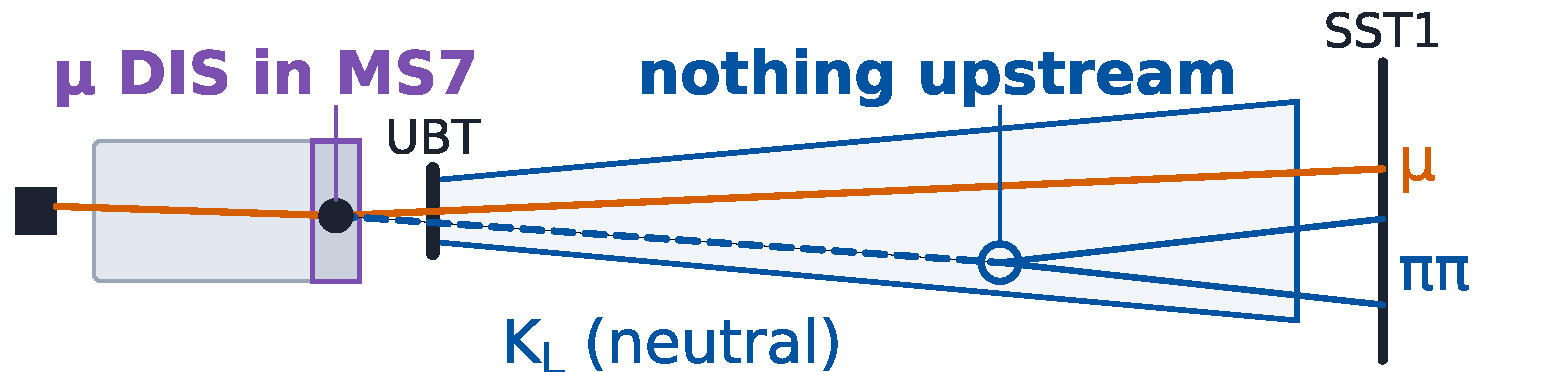
\includegraphics[width=1.00\linewidth,height=28.22pt,keepaspectratio]{figs/s02_sk1.pdf}\par}
\vspace{0.41pt}
{\fontsize{4.55pt}{6.15pt}\selectfont neutral: a K\textsubscript{L} made in the last iron of the shield decays in the vessel; nothing crosses the entrance\par}
\end{minipage}%
\hfill%
\begin{minipage}[t]{\dimexpr(0.5000\linewidth-0.5000\dimexpr11.49pt\relax)}\vspace{0pt}\raggedright
{\color{orange}\rule{\linewidth}{0.85pt}}\par\vspace{1.14pt}{\fontsize{5.23pt}{7.07pt}\selectfont \textcolor{orange}{\textbf{μ inelastic in the vessel}}\par}
\vspace{0.41pt}
{\centering 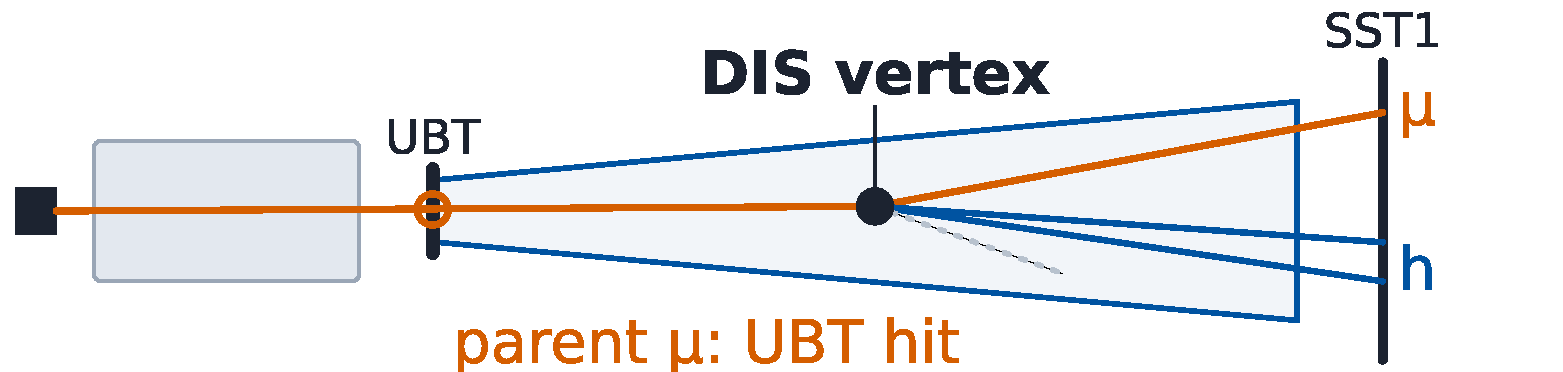
\includegraphics[width=1.00\linewidth,height=28.22pt,keepaspectratio]{figs/s02_sk2.pdf}\par}
\vspace{0.41pt}
{\fontsize{4.55pt}{6.15pt}\selectfont a real vertex in the helium or the walls; the parent muon crossed a tagger\par}
\end{minipage}\par
\vspace{1.37pt}
\noindent \begin{minipage}[t]{\dimexpr(0.5000\linewidth-0.5000\dimexpr11.49pt\relax)}\vspace{0pt}\raggedright
{\color{green}\rule{\linewidth}{0.85pt}}\par\vspace{1.14pt}{\fontsize{5.23pt}{7.07pt}\selectfont \textcolor{green}{\textbf{ν inelastic in the vessel and MS7}}\par}
\vspace{0.41pt}
{\centering 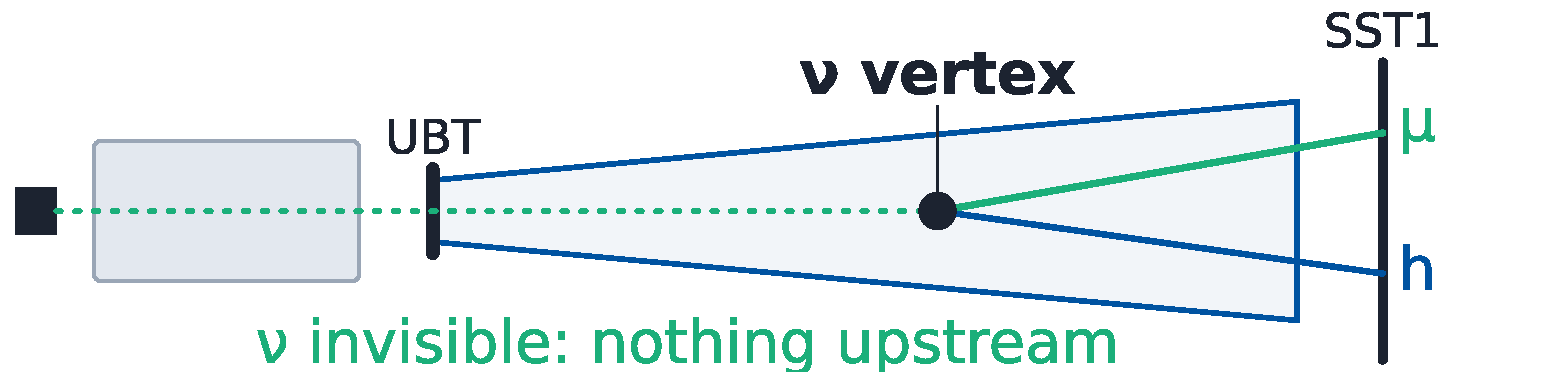
\includegraphics[width=1.00\linewidth,height=28.22pt,keepaspectratio]{figs/s02_sk3.pdf}\par}
\vspace{0.41pt}
{\fontsize{4.55pt}{6.15pt}\selectfont no incoming charged particle\par}
\end{minipage}%
\hfill%
\begin{minipage}[t]{\dimexpr(0.5000\linewidth-0.5000\dimexpr11.49pt\relax)}\vspace{0pt}\raggedright
{\color{cern}\rule{\linewidth}{0.85pt}}\par\vspace{1.14pt}{\fontsize{5.23pt}{7.07pt}\selectfont \textcolor{cern}{\textbf{combinatorial: μ × μ}}\par}
\vspace{0.41pt}
{\centering 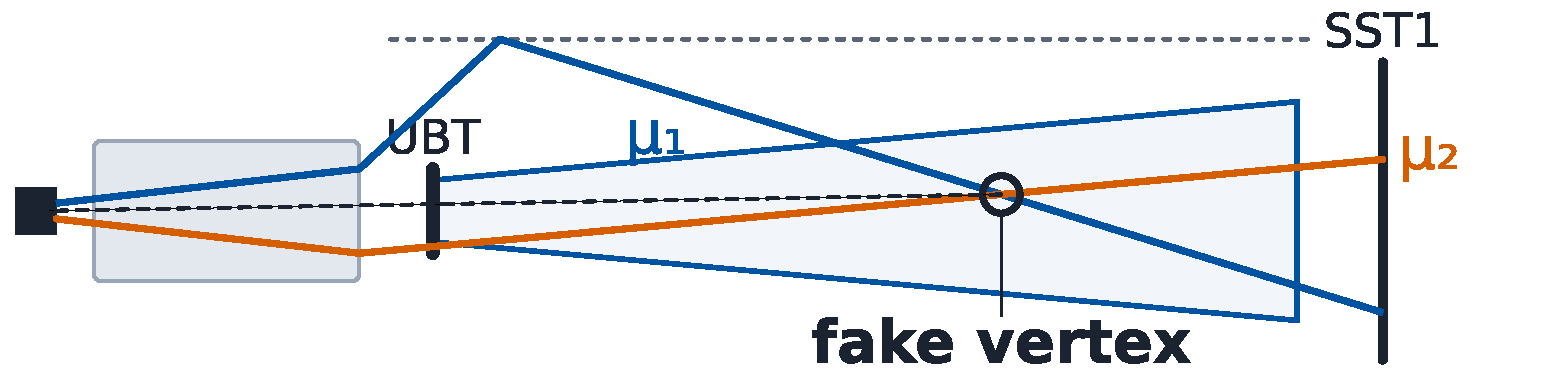
\includegraphics[width=1.00\linewidth,height=28.22pt,keepaspectratio]{figs/s02_sk4.pdf}\par}
\vspace{0.41pt}
{\fontsize{4.55pt}{6.15pt}\selectfont two muons from the target, in time by chance\par}
\end{minipage}\par
\vspace{1.37pt}
\noindent \begin{minipage}[t]{\dimexpr(0.5000\linewidth-0.5000\dimexpr11.49pt\relax)}\vspace{0pt}\raggedright
{\color{cern}\rule{\linewidth}{0.85pt}}\par\vspace{1.14pt}{\fontsize{5.23pt}{7.07pt}\selectfont \textcolor{cern}{\textbf{combinatorial: μ × interaction product}}\par}
\vspace{0.41pt}
{\centering 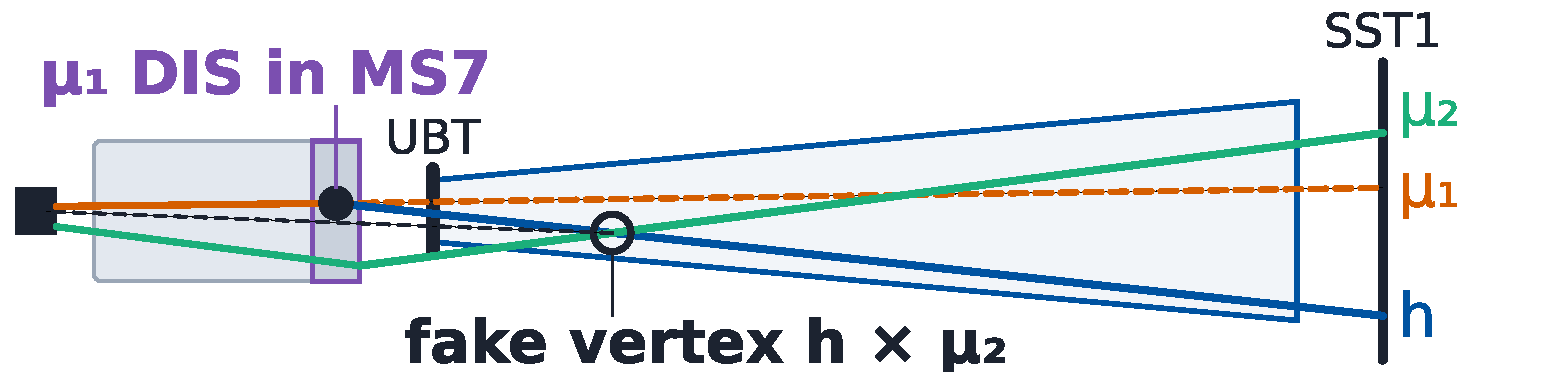
\includegraphics[width=1.00\linewidth,height=28.22pt,keepaspectratio]{figs/s02_sk5.pdf}\par}
\vspace{0.41pt}
{\fontsize{4.55pt}{6.15pt}\selectfont a muon with a charged product of an unrelated DIS (MS7, vessel)\par}
\end{minipage}%
\hfill%
\begin{minipage}[t]{\dimexpr(0.5000\linewidth-0.5000\dimexpr11.49pt\relax)}\vspace{0pt}\raggedright
{\color{cern}\rule{\linewidth}{0.85pt}}\par\vspace{1.14pt}{\fontsize{5.23pt}{7.07pt}\selectfont \textcolor{cern}{\textbf{combinatorial: μ × cavern-rock particle}}\par}
\vspace{0.41pt}
{\centering 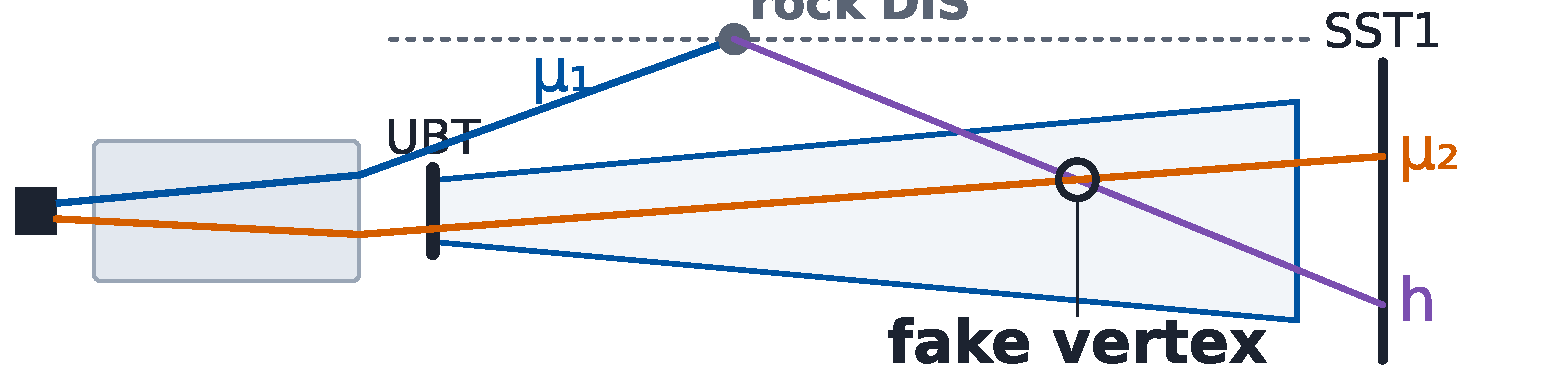
\includegraphics[width=1.00\linewidth,height=28.22pt,keepaspectratio]{figs/s02_sk6.pdf}\par}
\vspace{0.41pt}
{\fontsize{4.55pt}{6.15pt}\selectfont a muon with a hadron or electron from a muon interaction in the cavern rock\par}
\end{minipage}\par
\vspace{2.46pt}
{\fontsize{10.92pt}{14.99pt}\selectfont Inelastic = deep-inelastic and lower-energy muon–nucleus and ν–nucleus interactions. \\ Goal: \textbf{< 0.1 background events in 15 years} (6×10\textsuperscript{20} PoT).\par}
\end{btframe}

% ---------------------------------------------------------------- slide 4: Geometry in the simulation: FairShip 2026 layout
\begin{btframe}{1 · Introduction · geometry}{Geometry in the simulation: FairShip 2026 layout}
{\centering 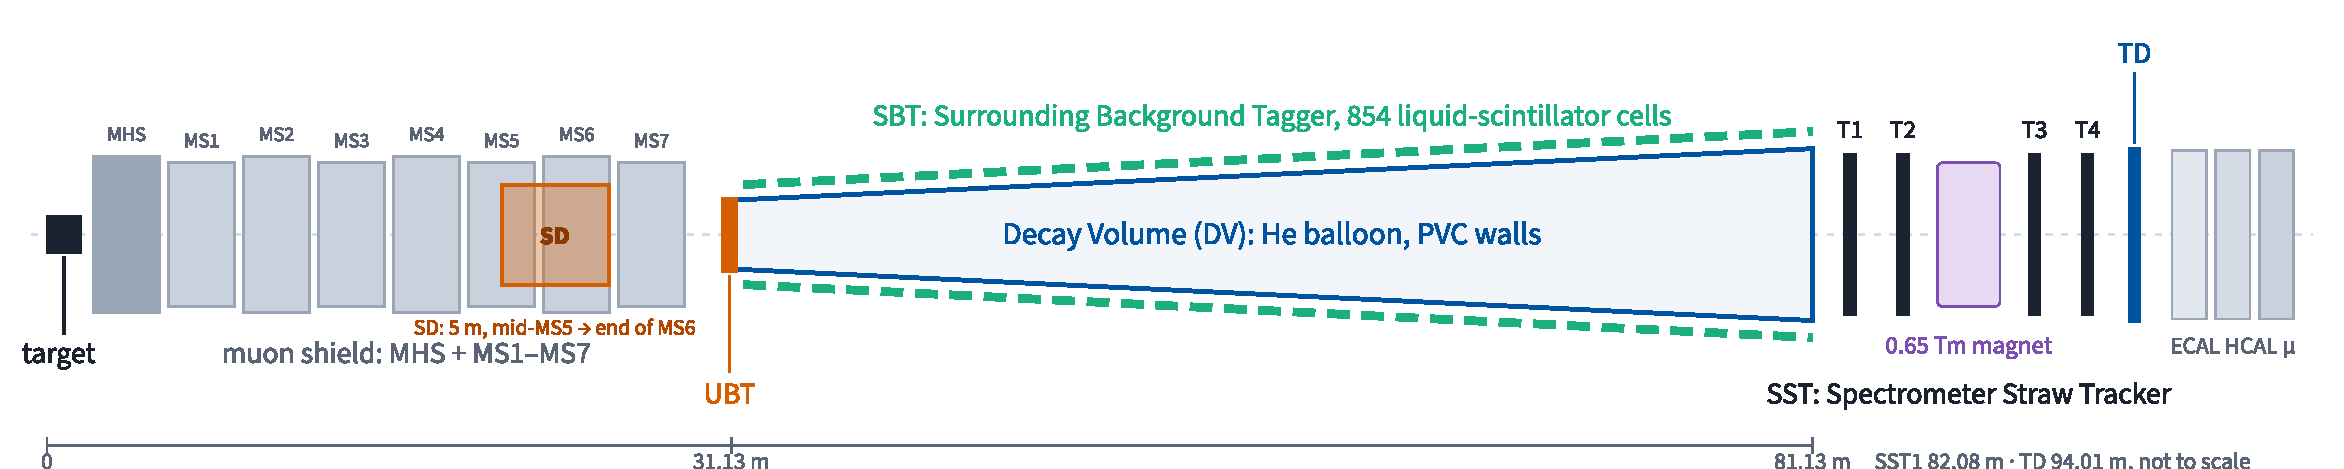
\includegraphics[width=1.00\linewidth,height=72.83pt,keepaspectratio]{figs/s03_sk1.pdf}\par}
\vspace{2.73pt}
{\fontsize{5.02pt}{6.52pt}\selectfont\setlength{\tabcolsep}{3.51pt}\renewcommand{\arraystretch}{1.42}
\begin{tabularx}{\linewidth}{l>{\raggedright\arraybackslash}Xl}
\textcolor{muted}{name} & \textcolor{muted}{what it is} & \textcolor{muted}{where} \\\headrule
MS & muon shield: MHS + MS1–MS7; MS7 = last magnet, iron z = 29.39–29.89 m & TRY6 (Nov-4 production) \\\rowrule
UBT & Upstream Background Tagger on the entrance window: vertical straws (1 × 2.7 m\textsuperscript{2}) + 4 × 4 m\textsuperscript{2} tile plane & z = 30.73 m (straws), 31.13 m (tiles) \\\rowrule
SBT & Surrounding Background Tagger: 20 cm liquid scintillator between 8 mm Al walls, 61 rings × 14 cells & z = 31.13 – 81.13 m \\\rowrule
DV & Decay Volume: frustum 1.0 × 2.7 m\textsuperscript{2} → 4 × 6 m\textsuperscript{2}, helium at 1 bar & z = 31.13 – 81.13 m \\\rowrule
SST, TD & spectrometer straw tracker (SST1 first station) and timing detector & SST1 82.08 m, TD 94.01 m \\\rowrule
MSMS & Muon Shield Monitoring System: silicon strip stations inside the MS7 iron (R3) & z = 29.39, 29.59, 29.79 m \\\rowrule
\end{tabularx}\par}
\slidenote{Names: CERN-SHiP-INT-2025-004 (Note\_combinatorial\_background, sec. 1, 3.1, 5). Source: veto lib/veto/geometry.py (FairShip geometry\_config 2026-0.1, target-aligned z = z\textsubscript{FS} − 2.14 m)}
\end{btframe}

% ---------------------------------------------------------------- slide 5: Initial sample: muons and neutrinos from the target
\begin{btframe}{1 · Introduction · the input}{Initial sample: muons and neutrinos from the target}
{\fontsize{4.55pt}{5.92pt}\selectfont\setlength{\tabcolsep}{3.19pt}\renewcommand{\arraystretch}{1.42}
\begin{tabularx}{\linewidth}{lrr>{\raggedright\arraybackslash}X>{\raggedright\arraybackslash}X}
\textcolor{muted}{sample} & \textcolor{muted}{source} & \textcolor{muted}{per spill (4×10\textsuperscript{13} PoT; stat. < 1 \%)} & \textcolor{muted}{transport} & \textcolor{muted}{stored / cuts} \\\headrule
muons & Nov-4 target pool (Shah Rukh, Nov 2026) & 4.70×10\textsuperscript{10} (μ\textsuperscript{+} 2.5×10\textsuperscript{10}, μ\textsuperscript{-} 2.2×10\textsuperscript{10}) & Cuda Muons through TRY6 + TCC8 rock + cavern, 3 220 seeds = 3 220 spills & states at z = 30.6 m and at SST1 (shell storage, 7.7×10\textsuperscript{8} rows) \\\rowrule
neutrinos & 2026 production (target + shield) & 4.2×10\textsuperscript{11} (ν\textsubscript{μ} 2.2×10\textsuperscript{11}, ν̄\textsubscript{μ} 1.6×10\textsuperscript{11}, ν\textsubscript{e} + ν̄\textsubscript{e} 4.3×10\textsuperscript{10}, ν\textsubscript{τ} + ν̄\textsubscript{τ} 3×10\textsuperscript{9}) & straight lines; GENIE 3.06 interactions forced in every target & E > 1 GeV, θ < 0.3 rad \\\rowrule
\end{tabularx}\par}
\vspace{2.46pt}
\noindent \begin{minipage}[t]{\dimexpr(0.5745\linewidth-0.5745\dimexpr9.67pt\relax)}\vspace{0pt}\raggedright
{\centering 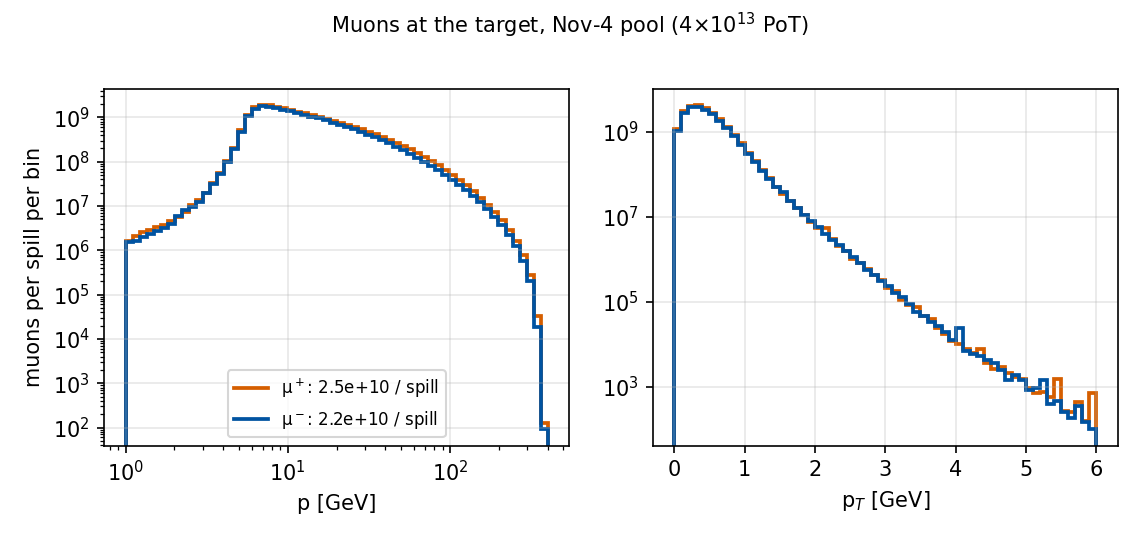
\includegraphics[width=1.00\linewidth,keepaspectratio]{figs/s04_img1.png}\par}
\end{minipage}%
\hfill%
\begin{minipage}[t]{\dimexpr(0.4255\linewidth-0.4255\dimexpr9.67pt\relax)}\vspace{0pt}\raggedright
{\centering 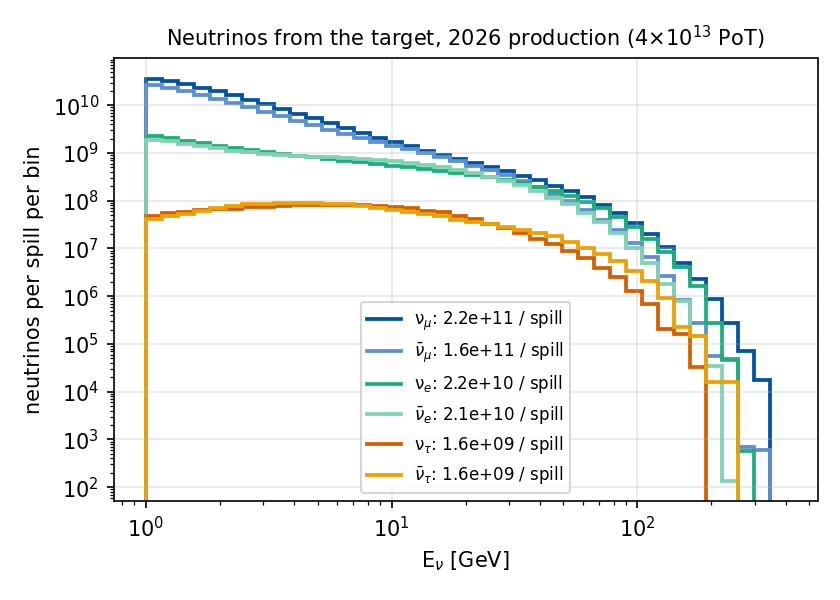
\includegraphics[width=1.00\linewidth,keepaspectratio]{figs/s04_img2.png}\par}
\end{minipage}\par
\vspace{2.46pt}
{\fontsize{6.02pt}{8.43pt}\selectfont
\begin{itemize}
  \item \textbf{Nov-4 production} (Shah Rukh), used for every number in this talk; one seed = the whole pool once = one spill of 4×10\textsuperscript{13} PoT; 15 years = 1.5×10\textsuperscript{7} spills
\end{itemize}}
\end{btframe}

% sections/01_simulation.tex: generated by newdeck/html2beamer.py from the HTML deck, then edited by hand

% ---------------------------------------------------------------- slide 6: Outline
\begin{btframe}{}{Outline}
\begin{outlinelist}
\outlineitem{1}{Introduction}{the background types, the geometry, the input muons and neutrinos}{0.35}
\outlineitem{2}{Simulation}{transport, inelastic scattering, technologies, hits and digitisation, signal generation}{1.00}
\outlineitem{3}{Selection}{track cuts, pair cuts and time coincidence}{0.35}
\outlineitem{4}{Backgrounds before tagging}{μ and ν inelastic scattering, MS7 K\textsubscript{L}, combinatorial pairs}{0.35}
\outlineitem{5}{Background tagging}{rules, V0 rule, SBT model, R1, R2, summary}{0.35}
\outlineitem{6}{Optimisation and conclusion}{genetic-algorithm search, the optimised designs Z2 and Z3}{0.35}
\end{outlinelist}
\end{btframe}

% ---------------------------------------------------------------- slide 7: Transport through the shield and the cavern: Cuda Muons
\begin{btframe}{2 · Simulation · transport}{Transport through the shield and the cavern: Cuda Muons}
{\centering 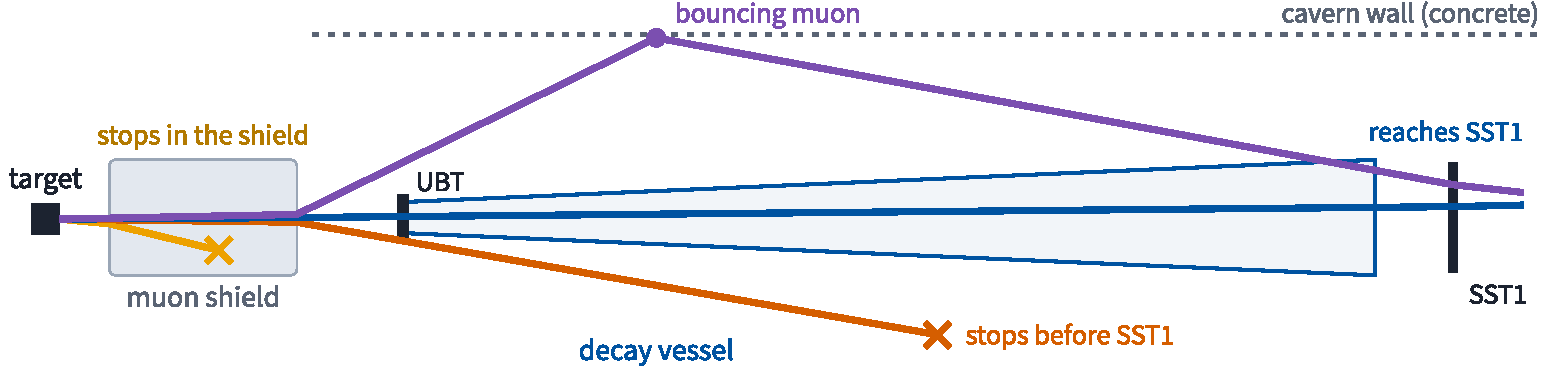
\includegraphics[width=1.00\linewidth,height=59.18pt,keepaspectratio]{figs/s06_sk1.pdf}\par}
\vspace{2.46pt}
\noindent \begin{minipage}[t]{\dimexpr(0.4651\linewidth-0.4651\dimexpr11.49pt\relax)}\vspace{0pt}\raggedright
{\centering 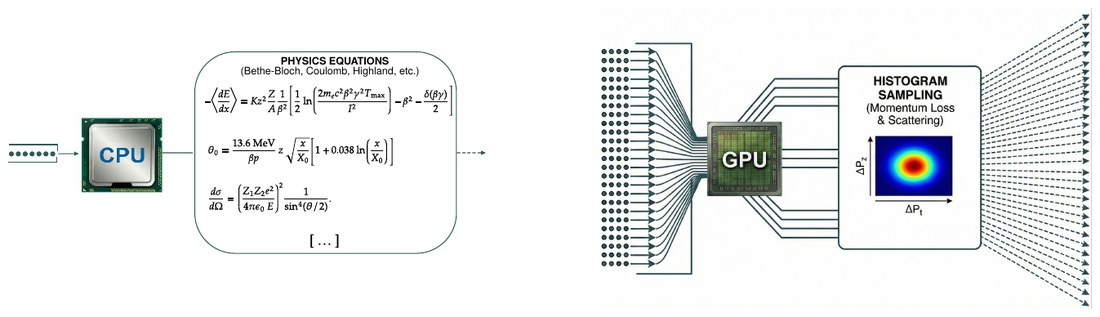
\includegraphics[width=1.00\linewidth,keepaspectratio]{figs/s06_img2.jpg}\par}
{\color{muted}\fontsize{5.48pt}{8.71pt}\selectfont Geant4 on a CPU, one muon at a time (left) vs Cuda Muons on a GPU (right)\par}
\vspace{2.46pt}
% {\centering 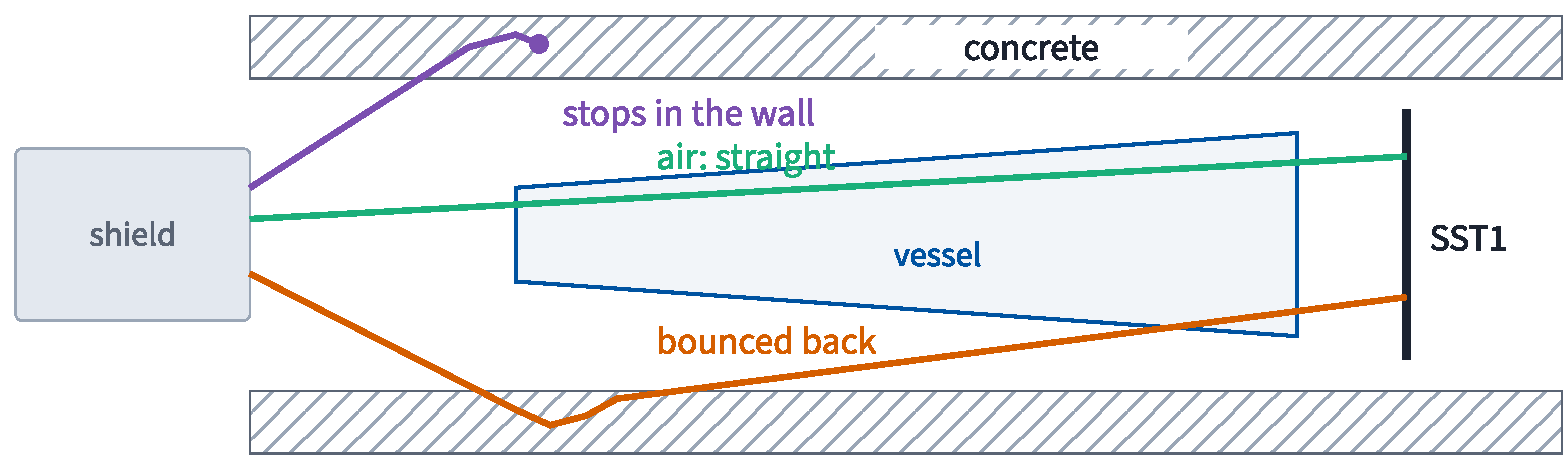
\includegraphics[width=1.00\linewidth,height=54.62pt,keepaspectratio]{figs/s06_sk3.pdf}\par}
\end{minipage}%
\hfill%
\begin{minipage}[t]{\dimexpr(0.5349\linewidth-0.5349\dimexpr11.49pt\relax)}\vspace{0pt}\raggedright
{\fontsize{5.92pt}{8.03pt}\selectfont
\begin{itemize}
  \item[\status{blue}] Offline: Geant4 fills per-material histograms of momentum loss and p\textsubscript{T} kick for a fixed 2 cm step (95 log bins, 0.18–400 GeV)
  \item[\status{blue}] Online: one CUDA thread per muon samples them in O(1) (alias method); field integrated with RK4
    \item[\status{blue}] Nov-4 production (Shah Rukh): the Nov-4 target pool transported through the TRY6 shield and the cavern 3 220 times, one seed = one spill
    \item[\status{blue}] Stored: each muon’s state @UBT and @SST1
  \item[\status{green}] One GPU: >10\textsuperscript{4}× faster than single-core Geant4, >100× faster than 1024 CPU cores
  \item[\status{red}] Decays are not simulated
  \item[\status{red}] Air is not simulated: muons travel in straight lines through the cavern air

\end{itemize}}
\end{minipage}\par
\slidenote{L. F. P. Cattelan, S. R. Qasim, P. H. Owen, N. Serra, “Ultra-Fast Muon Transport via Histogram Sampling on GPUs”, arXiv:2512.10520 (2025).}
\end{btframe}

% ---------------------------------------------------------------- slide 8: How an inelastic interaction is made: seven steps
\begin{btframe}{2 · Simulation · inelastic scattering}{How an inelastic interaction is made: seven steps}
\begin{flowrow}{\dimexpr(\linewidth-6\dimexpr6.37pt\relax)/7\relax}{6.37pt}%
\flowstep{white}{rule}{2.28pt}{3.64pt}{{\fontsize{5.92pt}{7.40pt}\selectfont\textbf{\textcolor{cern}{1 · parents}}\par}\vspace{0.91pt}{\fontsize{5.01pt}{6.76pt}\selectfont\textcolor{ink}{muons from the Nov-4 transport, ν from the 2026 flux, straight through each target}\par}}%
\flowarrow%
\flowstep{white}{rule}{2.28pt}{3.64pt}{{\fontsize{5.92pt}{7.40pt}\selectfont\textbf{\textcolor{cern}{2 · cross section}}\par}\vspace{0.91pt}{\fontsize{5.01pt}{6.76pt}\selectfont\textcolor{ink}{Kokoulin per nucleon (μ), GENIE splines (ν)}\par}}%
\flowarrow%
\flowstep{white}{rule}{2.28pt}{3.64pt}{{\fontsize{5.92pt}{7.40pt}\selectfont\textbf{\textcolor{cern}{3 · forced}}\par}\vspace{0.91pt}{\fontsize{5.01pt}{6.76pt}\selectfont\textcolor{ink}{one interaction per crossing, weight w·P = interactions per spill}\par}}%
\flowarrow%
\flowstep{white}{rule}{2.28pt}{3.64pt}{{\fontsize{5.92pt}{7.40pt}\selectfont\textbf{\textcolor{cern}{4 · generator}}\par}\vspace{0.91pt}{\fontsize{5.01pt}{6.76pt}\selectfont\textcolor{ink}{Geant4 muonNuclear + Pythia 6 (μ), GENIE 3.06 (ν)}\par}}%
\flowarrow%
\flowstep{white}{rule}{2.28pt}{3.64pt}{{\fontsize{5.92pt}{7.40pt}\selectfont\textbf{\textcolor{cern}{5 · short-lived}}\par}\vspace{0.91pt}{\fontsize{5.01pt}{6.76pt}\selectfont\textcolor{ink}{K\textsubscript{S}, Λ, π\textsuperscript{0} … decayed; in MS7 handed to Geant4}\par}}%
\flowarrow%
\flowstep{white}{rule}{2.28pt}{3.64pt}{{\fontsize{5.92pt}{7.40pt}\selectfont\textbf{\textcolor{cern}{6 · transport}}\par}\vspace{0.91pt}{\fontsize{5.01pt}{6.76pt}\selectfont\textcolor{ink}{straight to SST1 with scattering (vessel); Geant4 + field map through the MS7 iron}\par}}%
\flowarrow%
\flowstep{white}{rule}{2.28pt}{3.64pt}{{\fontsize{5.92pt}{7.40pt}\selectfont\textbf{\textcolor{cern}{7 · selection, tagging}}\par}\vspace{0.91pt}{\fontsize{5.01pt}{6.76pt}\selectfont\textcolor{ink}{as for the muon pairs; own and random hits}\par}}%
\end{flowrow}
\vspace{2.46pt}
\noindent \begin{minipage}[[c]{0.5\linewidth}
{\fontsize{4.55pt}{6.15pt}\selectfont \textcolor{cern}{\textbf{2 · cross section: μ, per nucleon in iron}}\par}
\vspace{0.55pt}
{\centering 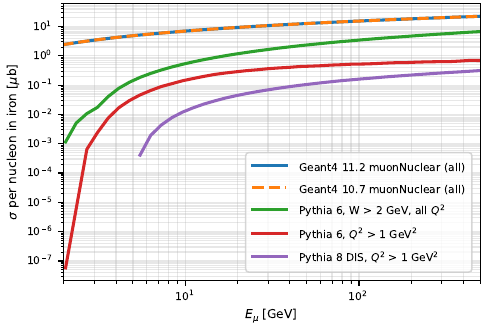
\includegraphics[height=86.49pt,keepaspectratio]{figs/s07_img1.png}\par}
\end{minipage}%
\hfill%
\begin{minipage}[c]{0.5\linewidth}
{\fontsize{4.55pt}{6.15pt}\selectfont \textcolor{cern}{\textbf{2 · cross section: ν, σ/E per nucleon on \textsuperscript{56}Fe}}\par}
\vspace{0.55pt}
{\centering 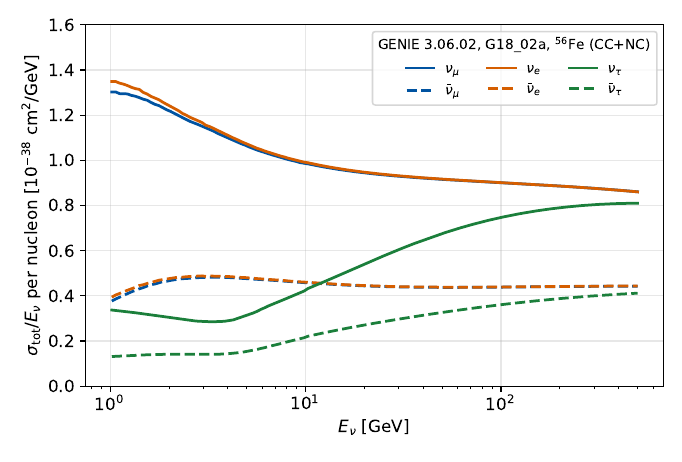
\includegraphics[height=86.49pt,keepaspectratio]{figs/s07_img2.png}\par}
\end{minipage}%
\hfill%
\vspace{2.46pt}
{\fontsize{4.55pt}{6.15pt}\selectfont \centering \textcolor{cern}{\textbf{3 · forced interaction}}\par}
\vspace{0.82pt}
{\centering 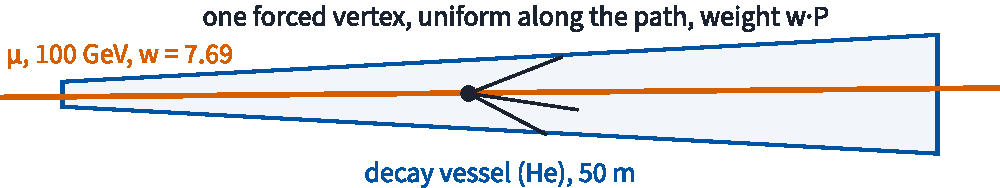
\includegraphics[width=1.00\linewidth,height=29.59pt,keepaspectratio]{figs/s07_sk3.pdf}\par}
\vspace{0.82pt}
{\fontsize{4.78pt}{6.45pt}\selectfont \centering P = n σ L along the crossing (helium, 10 GeV: 4×10\textsuperscript{-6}); the vertex is forced, the event weight w·P = interactions per spill\par}

\end{btframe}

% ---------------------------------------------------------------- slide 9: Detector technologies and the cost unit: the drachma
\begin{btframe}{2 · Simulation · technologies}{Detector technologies and the cost unit: the drachma}
{\fontsize{6.36pt}{8.66pt}\selectfont\setlength{\tabcolsep}{3.05pt}\renewcommand{\arraystretch}{1.42}
\begin{tabularx}{\linewidth}{>{\raggedright\arraybackslash}Xrrrr}
\textcolor{muted}{} & \textcolor{muted}{straw (UBT)} & \textcolor{muted}{tile} & \textcolor{muted}{tile2 (flames)} & \textcolor{muted}{LS + WOM (SBT)} \\\headrule
layers & 6 (vertical) & 1 & 1 & LS cell 20 cm \\\rowrule
cell & 5 mm & 4 × 4 cm\textsuperscript{2} & 2 × 2 cm\textsuperscript{2} & 80 × ≤150 cm\textsuperscript{2} \\\rowrule
σ\textsubscript{t} / window & drift, ±25 ns & 120 ps, ±3σ & 90 ps, ±3σ & \textasciitilde{}1 ns, ±3 ns \\\rowrule
efficiency & 99.9 \% & 99.9 \% & 99.9 \% & 99.3 \% \\\rowrule
X / X\textsubscript{0} & 0.12 \% & 2.4 \% & 2.4 \% & \textasciitilde{}40 \% \\\rowrule
cost / m\textsuperscript{2} (drachmas) & 2.9 & 4.0 & 16.9 & \textasciitilde{}0.34 \\\rowrule
\end{tabularx}\par}

\vspace{2.46pt}
\noindent
\begin{minipage}[c]{0.6\linewidth}
    \raggedright
    {\fontsize{6.15pt}{8.30pt}\selectfont
    \textcolor{cern}{\textbf{R2 = 333.5 drachmas = the budget
    \textcolor{muted}{{\fontsize{4.61pt}{5.99pt}\selectfont
    (R1 99.7)}}}}\par}
    \vspace{2.46pt}
    {\centering
    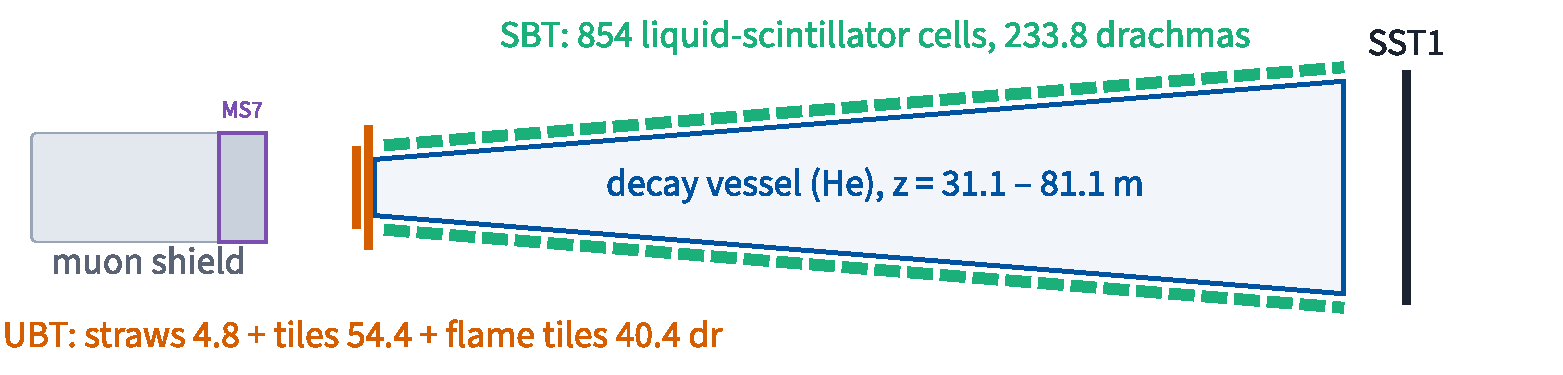
\includegraphics[width=\linewidth,keepaspectratio]
    {figs/s08_sk3.pdf}\par}
\end{minipage}%
\hfill
\begin{minipage}[c]{0.125\linewidth}
    \centering
    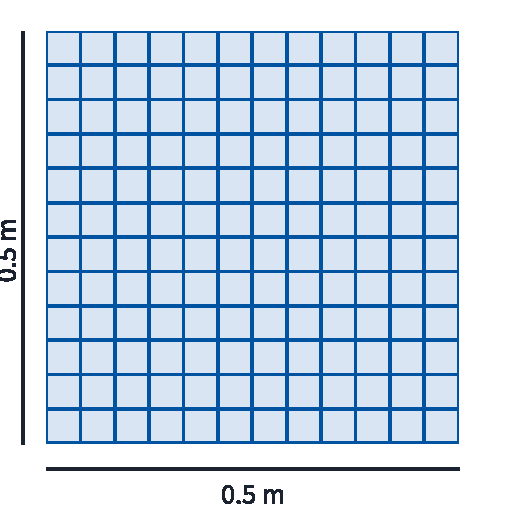
\includegraphics[width=\linewidth,keepaspectratio]
    {figs/s08_sk1.pdf}
\end{minipage}%
\hfill
\begin{minipage}[c]{0.04\linewidth}
    \centering
    {\fontsize{13.66pt}{18.44pt}\selectfont
    \textcolor{cern}{\textbf{=}}}
\end{minipage}%
\hfill
\begin{minipage}[c]{0.145\linewidth}
    \centering
    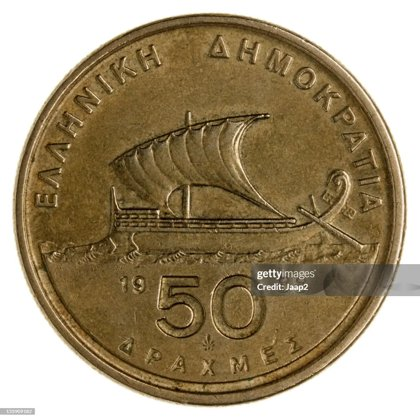
\includegraphics[width=\linewidth,keepaspectratio]
    {figs/s08_img2.jpg}
\end{minipage}%
\par
% \hfill%
\vspace{2.46pt}
\noindent 
% \begin{minipage}[c]{\dimexpr(0.2500\linewidth-0.2500\dimexpr16.96pt\relax)}\raggedright
{\fontsize{6.02pt}{8.43pt}\selectfont
\begin{itemize}
  \item \textbf{1 drachma} = the cost of one 0.5 × 0.5 m\textsuperscript{2} module of 4 × 4 cm\textsuperscript{2} tiles (144 tiles)
  \item Relative costs from one placeholder model: channels × relative cost per channel + 10 \% mechanics; never absolute money
\end{itemize}}
% \end{minipage}\par

\end{btframe}


% ---------------------------------------------------------------- slide 10: Hits and digitisation: own hits, random hits, time windows
\begin{btframe}{2 · Simulation · hits and digitisation}{Hits and digitisation: own hits, random hits, time windows}
{\fontsize{6.02pt}{7.52pt}\selectfont\setlength{\tabcolsep}{3.51pt}\renewcommand{\arraystretch}{1.42}
\begin{tabularx}{\linewidth}{lrr>{\raggedright\arraybackslash}Xr}
\textcolor{muted}{plane} & \textcolor{muted}{cell} & \textcolor{muted}{time window} & \textcolor{muted}{position} & \textcolor{muted}{efficiency} \\\headrule
UBT straws & 6 layers, vertical, 5 mm & 50 ns drift: ±25 ns & no position along the 0.9 m section & 99.9 \% \\\rowrule
UBT tiles & 4 × 4 cm\textsuperscript{2} (2 × 2 cm\textsuperscript{2} in the flames) & ±3σ (σ 120 / 90 ps) & cell centre & 99.9 \% \\\rowrule
SBT cells & 854 LS cells, 20 cm, 30 MeV threshold & \textasciitilde{}1 ns, ±3 ns & cell + pointing along the wall & 99.3 \% \\\rowrule
\end{tabularx}\par}
\vspace{2.46pt}
\noindent \begin{minipage}[c]{0.5\linewidth}
{\centering 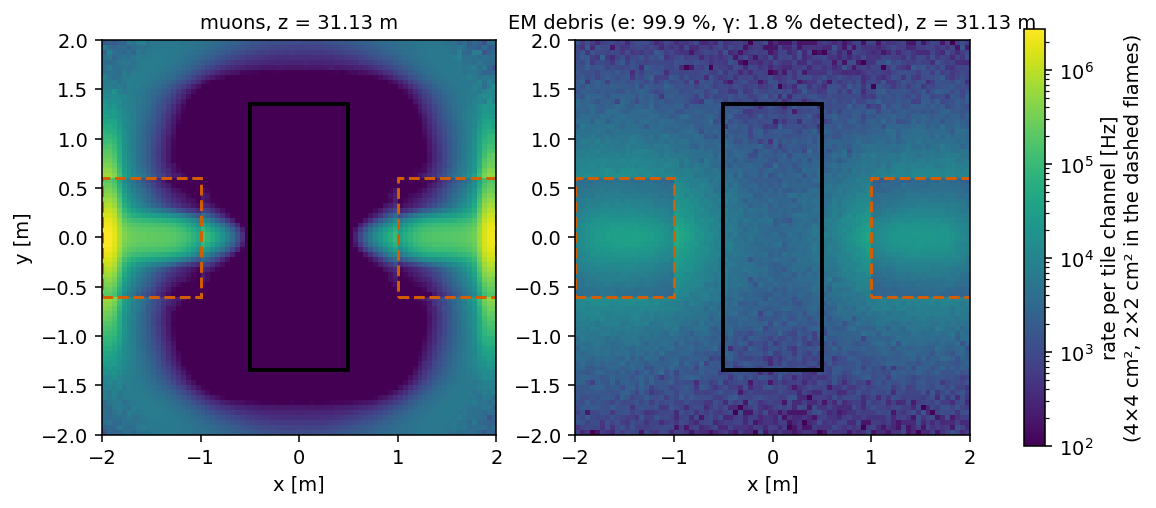
\includegraphics[width=1\linewidth,keepaspectratio]{figs/s09_img1.png}\par}
\end{minipage}%
\hfill%
\begin{minipage}[c]{0.5\linewidth}
{\fontsize{6.02pt}{8.43pt}\selectfont
\begin{itemize}
  \item \textbf{Own hits:} each simulated particle is crossed with every plane; a hit if the cell fires (efficiency, threshold, energy deposit in the LS)
  \item \textbf{Random hits:} all the other muons of the spill, Poisson from full-statistics rate maps, 
  \begin{equation*}
      \langle N_\text{acc}\rangle  = R_\text{plane} · 2W / 1 s
  \end{equation*}
  \item \textbf{EM debris} of the shield end (e / γ) added to the UBT rate maps
  \item \textbf{Scattering} in the vessel walls and the SBT shell, mean \textbf{energy loss} in the shell (soft muons stop)
  \item A track is \textbf{tagged} by a hit in its space–time window on any plane upstream of its vertex
  \item Tile plane: up to 2.8 MHz per channel from muons in the flames, ≤ 53 kHz from EM debris; mean random hits per tile in ±0.36 ns: 2×10\textsuperscript{-3} (μ), 4×10\textsuperscript{-5} (EM)
\end{itemize}}
\end{minipage}\par
\slidenote{$N_\text{acc}$ is the mean number of accidental hits. The actual number is drawn from a Poisson distribution with that mean, independently for each event. $R_\text{plane}$ the total rate of hits on the whole plane, The maps are built from the full muon sample, EM debris included, and the SBT uses ×4 itssimulated rate.  - 2W: the full width of the time window the plane is read in. W is the half-width; for    tiles the window is ±1.5 ns, so 2W = 3 ns.}
\end{btframe}

% ---------------------------------------------------------------- slide 11: Signal: truth-level generation with EventCalc
\begin{btframe}{2 · Simulation · signal}{Signal: truth-level generation with EventCalc}
\begin{flowrow}{\dimexpr(\linewidth-3\dimexpr6.37pt\relax)/4\relax}{6.37pt}%
\flowstep{white}{rule}{2.28pt}{3.64pt}{{\fontsize{5.92pt}{7.40pt}\selectfont\textbf{\textcolor{cern}{production}}\par}\vspace{0.91pt}{\fontsize{5.91}{6.76pt}\selectfont\textcolor{ink}{tabulated P(θ, E) per proton;\\ LLP from the target centre, straight}\par}}%
\flowarrow%
\flowstep{white}{rule}{2.28pt}{3.64pt}{{\fontsize{5.92pt}{7.40pt}\selectfont\textbf{\textcolor{cern}{decay vertex}}\par}\vspace{0.91pt}{\fontsize{5.91}{6.76pt}\selectfont\textcolor{ink}{exponential in the decay volume, weight P\textsubscript{decay}}\par}}%
\flowarrow%
\flowstep{white}{rule}{2.28pt}{3.64pt}{{\fontsize{5.92pt}{7.40pt}\selectfont\textbf{\textcolor{cern}{decay}}\par}\vspace{0.91pt}{\fontsize{5.91}{6.76pt}\selectfont\textcolor{ink}{all channels of the model (423 blocks), Pythia for the hadrons}\par}}%
\flowarrow%
\flowstep{white}{rule}{2.28pt}{3.64pt}{{\fontsize{5.92pt}{7.40pt}\selectfont\textbf{\textcolor{cern}{to tracks}}\par}\vspace{0.91pt}{\fontsize{5.91}{6.76pt}\selectfont\textcolor{ink}{daughters through field and matter to SST1 and the TD, then the same selection}\par}}%
\end{flowrow}
\vspace{2.46pt}
\noindent \begin{minipage}[c]{0.5\linewidth}
{\fontsize{6.11pt}{6.34pt}\selectfont\setlength{\tabcolsep}{2.88pt}\renewcommand{\arraystretch}{1.42}
\begin{tabular}{llr}
\textcolor{muted}{model} & \textcolor{muted}{coupling} & \textcolor{muted}{masses [GeV]} \\\headrule
HNL & pure e mixing; pure μ mixing & 0.5, 1, 2, 3, 4 \\\rowrule
dark photon & kinetic mixing, primary + cascade production & 0.3, 0.9, 2, 4 \\\rowrule
Higgs-like scalar & mixing with the Higgs & 0.5, 1, 2, 4 \\\rowrule
ALP & coupling to fermions & 0.5, 1, 2, 4 \\\rowrule
\end{tabular}\par}
\end{minipage}%
\hfill%
\begin{minipage}[c]{0.5\linewidth}
{\fontsize{6.11pt}{6.34pt}\selectfont\setlength{\tabcolsep}{2.88pt}\renewcommand{\arraystretch}{1.42}
\begin{tabularx}{\linewidth}{l>{\raggedright\arraybackslash}Xr}
\textcolor{muted}{model} & \textcolor{muted}{two-body} & \textcolor{muted}{three-body (missing ν / π\textsuperscript{0})} \\\headrule
HNL & N → π\textsuperscript{±} ℓ\textsuperscript{\ensuremath{\mp}} (full) & N → ℓ\textsuperscript{+} ℓ\textsuperscript{−} ν (partial) \\\rowrule
dark photon & A′ → μ\textsuperscript{+} μ\textsuperscript{−}, e\textsuperscript{+} e\textsuperscript{−} (full) & A′ → π\textsuperscript{+} π\textsuperscript{−} π\textsuperscript{0} (partial) \\\rowrule
scalar & S → π\textsuperscript{+} π\textsuperscript{−}, K\textsuperscript{+} K\textsuperscript{−}, μ\textsuperscript{+} μ\textsuperscript{−} (full) & – \\\rowrule
ALP & a → μ\textsuperscript{+} μ\textsuperscript{−} (full) & a → π\textsuperscript{+} π\textsuperscript{−} π\textsuperscript{0}, η π π (partial) \\\rowrule
\end{tabularx}\par}
\end{minipage}\par
\vspace{2.46pt}
{\centering {\centering 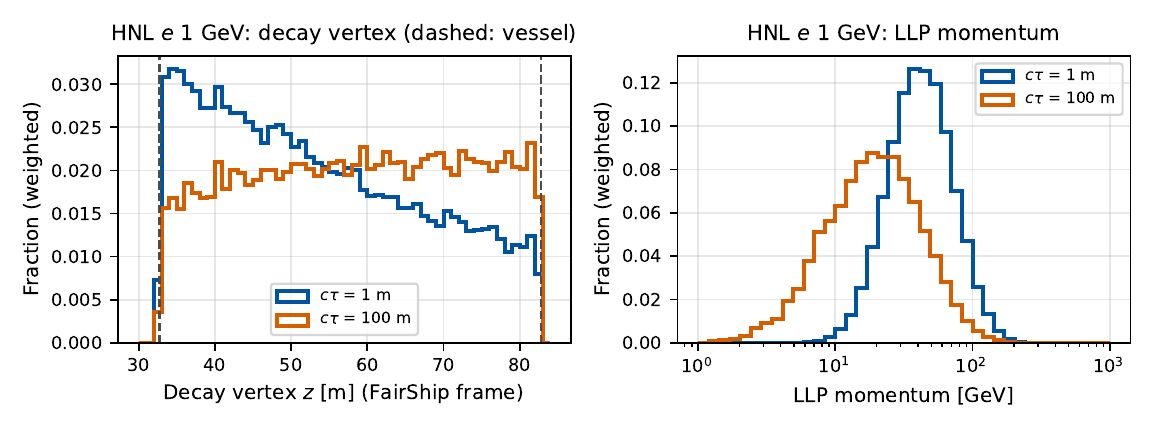
\includegraphics[height=109.04pt,keepaspectratio]{figs/s10_img1.png}\par}
\noindent
{\fontsize{6.78pt}{7.45pt}\selectfont cτ = 1 m and 100 m; 5×10\textsuperscript{4} LLPs per point, 3–4.5×10\textsuperscript{4} decaying in the vessel; efficiencies P\textsubscript{decay}-weighted\par}
\par}
\end{btframe}

% sections/02_selection.tex: generated by newdeck/html2beamer.py from the HTML deck, then edited by hand

% ---------------------------------------------------------------- slide 12: Outline
\begin{btframe}{}{Outline}
\begin{outlinelist}
\outlineitem{1}{Introduction}{the background types, the geometry, the input muons and neutrinos}{0.35}
\outlineitem{2}{Simulation}{transport, inelastic scattering, technologies, hits and digitisation, signal generation}{0.35}
\outlineitem{3}{Selection}{track cuts, pair cuts and time coincidence}{1.00}
\outlineitem{4}{Backgrounds before tagging}{μ and ν inelastic scattering, MS7 K\textsubscript{L}, combinatorial pairs}{0.35}
\outlineitem{5}{Background tagging}{rules, V0 rule, SBT model, R1, R2, summary}{0.35}
\outlineitem{6}{Optimisation and conclusion}{genetic-algorithm search, the optimised designs Z2 and Z3}{0.35}
\end{outlinelist}
\end{btframe}

% ---------------------------------------------------------------- slide 13: Track cuts: what a good track is
\begin{btframe}{3 · Selection · tracks}{Track cuts: what a good track is}
\noindent \begin{minipage}[c]{0.4\linewidth}
{\centering 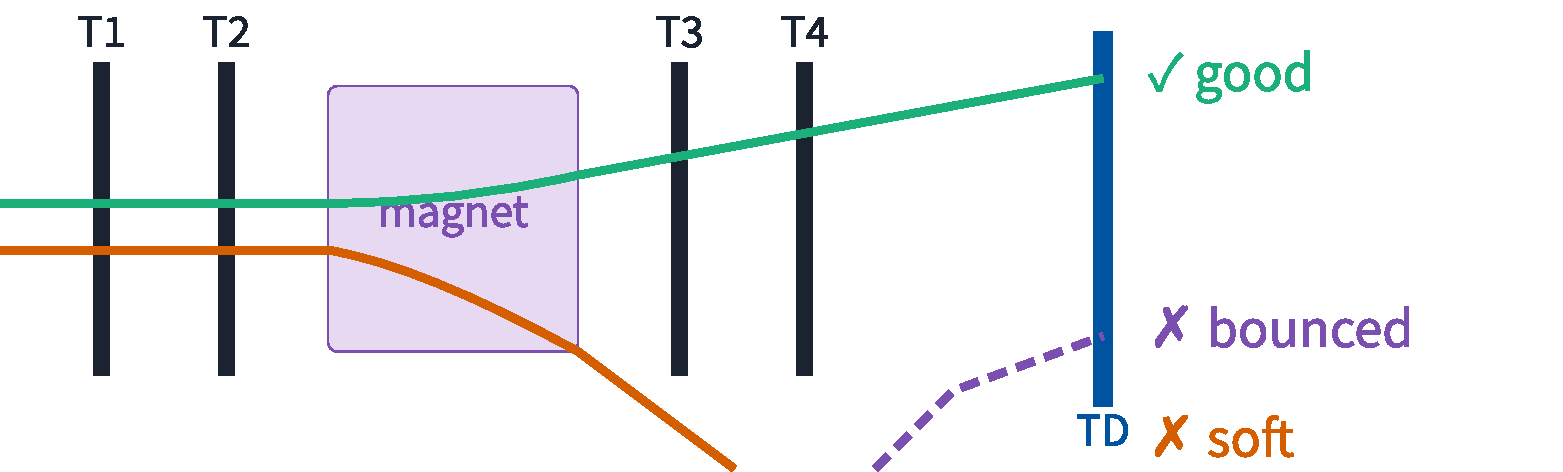
\includegraphics[width=1.00\linewidth,keepaspectratio]{figs/s12_sk1.pdf}\par}
\end{minipage}%
\hfill%
\begin{minipage}[c]{0.6\linewidth}
{\centering 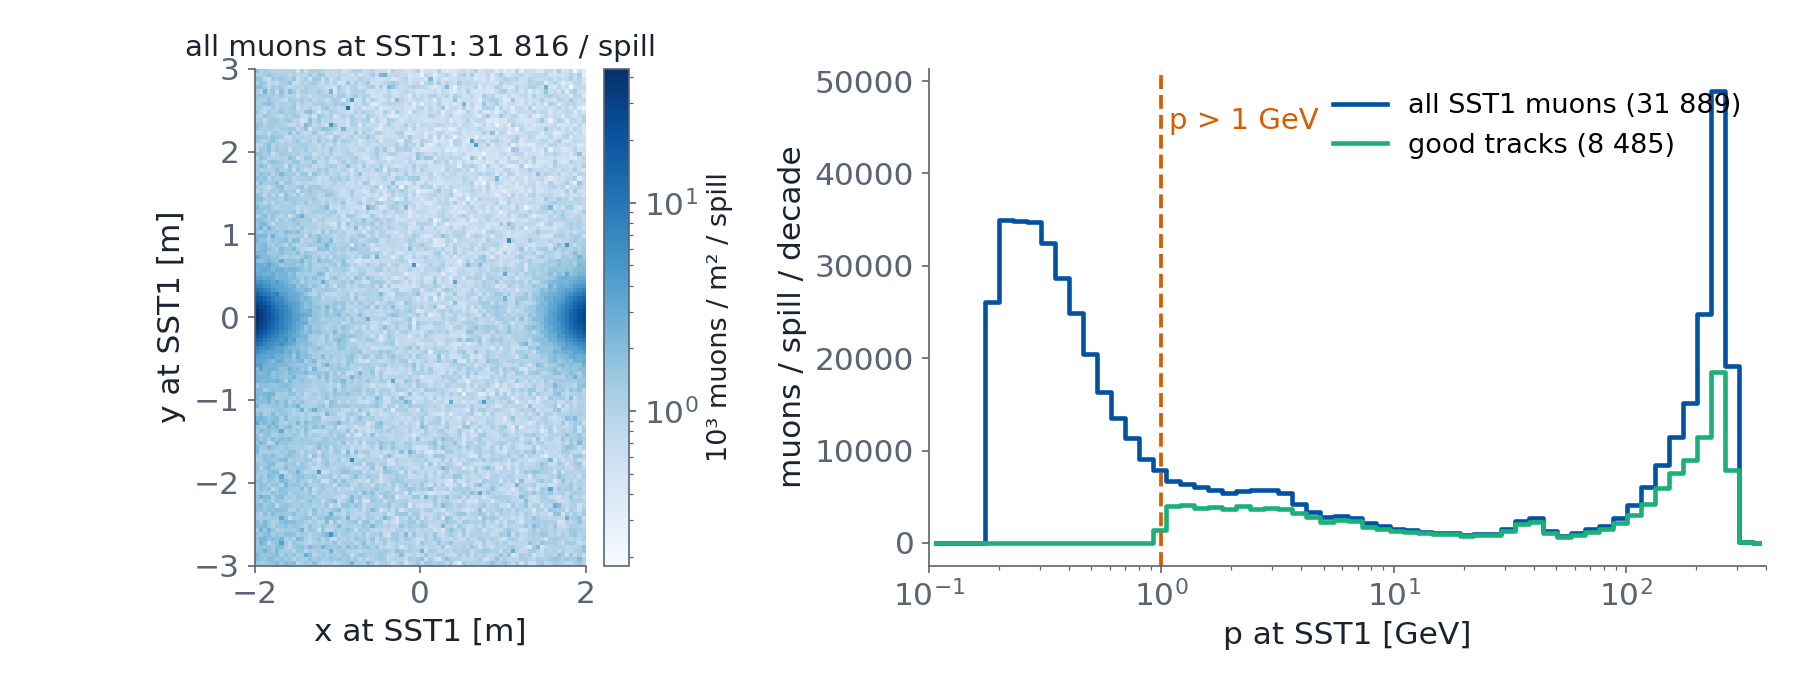
\includegraphics[width=1.00\linewidth]{figs/s12_img2.png}\par}
\end{minipage}\par
\vspace{2.46pt}
{\fontsize{6.02pt}{7.83pt}\selectfont\setlength{\tabcolsep}{4.21pt}\renewcommand{\arraystretch}{1.42}
\begin{tabularx}{\linewidth}{ll>{\raggedright\arraybackslash}Xr}
\textcolor{muted}{\#} & \textcolor{muted}{cut} & \textcolor{muted}{value} & \textcolor{muted}{muons / spill} \\\headrule
1 & SST1 acceptance & |x| < 2, |y| < 3 m at z = 82.08 m & 31.9 kHz \\\rowrule
2 & timing-detector acceptance & through the field map to z = 94.01 m, |x| < 2.75, |y| < 3.25 m &  \\\rowrule
3 & momentum & p > 1 GeV & 8.5 kHz good tracks (8.17 straight + 0.38 bounced) \\\rowrule
– & track quality (ACTS) & converged, n\textsubscript{dof} > 25, χ\textsuperscript{2}/n\textsubscript{dof} < 5 & not yet measured (option, not applied) \\\rowrule
\end{tabularx}\par}
\end{btframe}

% ---------------------------------------------------------------- slide 14: Pair cuts: opposite charge, DOCA, vertex, IP
\begin{btframe}{3 · Selection · pair cuts}{Pair cuts: opposite charge, DOCA, vertex, IP}
\noindent \begin{minipage}[c]{0.75\linewidth}
{\centering 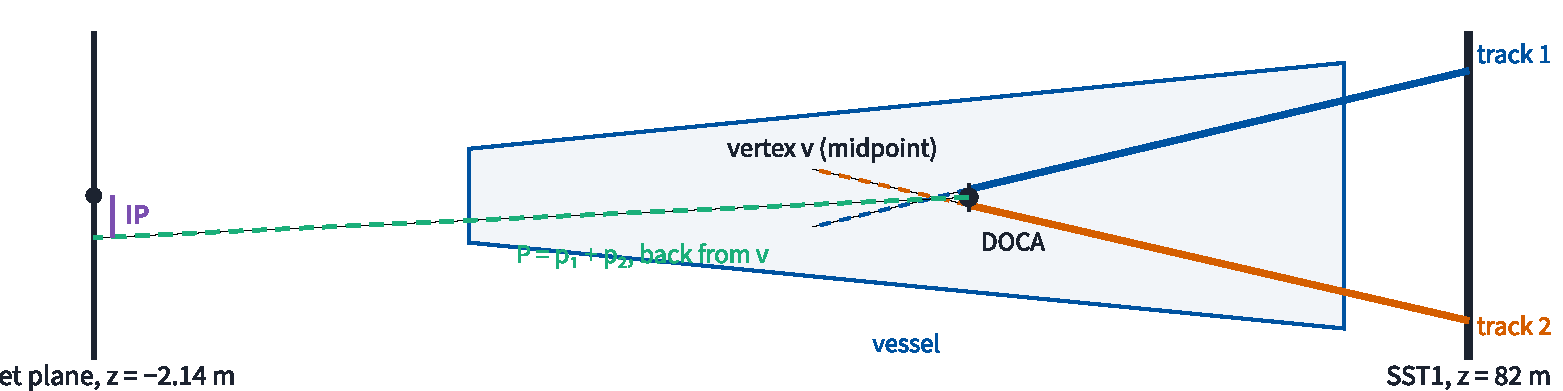
\includegraphics[width=1.00\linewidth,height=54.62pt,keepaspectratio]{figs/s13_sk1.pdf}\par}
\end{minipage}%
\hfill%
\begin{minipage}[c]{0.25\linewidth}
\begin{mathbox}[cern]{4.55pt}
\[\mathrm{DOCA} = \frac{\left|\,\Delta\vec r\cdot(\vec p_1\times\vec p_2)\,\right|}{\left|\vec p_1\times\vec p_2\right|}\]
\end{mathbox}
\vspace{1.64pt}
\begin{mathbox}[cern]{4.32pt}
\[\begin{aligned} \vec P &= \vec p_1 + \vec p_2 \\ \mathrm{IP} &= \left|\,\vec v_{xy} + \frac{\vec P_{xy}}{P_z}\,(-2.14\,\mathrm{m} - v_z)\right| \end{aligned}\]
\end{mathbox}
\end{minipage}\par
\vspace{2.46pt}
{\centering 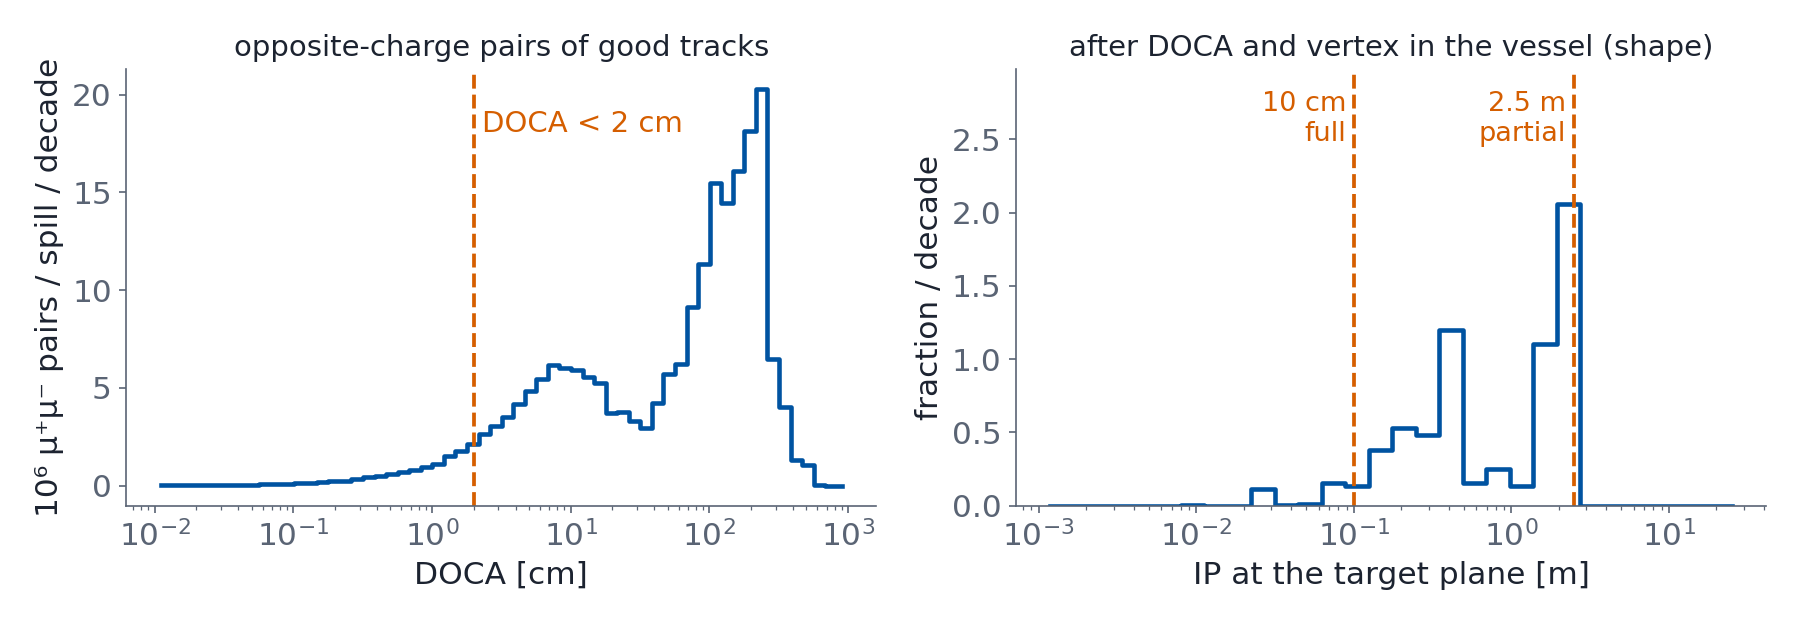
\includegraphics[width=0.66\linewidth]{figs/s13_img2.png}\par}
\vspace{2.46pt}
{\centering \fontsize{7.01pt}{8.76pt}\selectfont \textbf{Time}: two unrelated muons must agree within ±200 ps (TD, σ\textsubscript{t} = 100 ps) over a 1 s spill → factor 2 × 200 ps / 1 s = \textbf{4×10\textsuperscript{-10}}.\par}
\end{btframe}

% sections/03_backgrounds_before_tagging.tex: generated by newdeck/html2beamer.py from the HTML deck, then edited by hand

% ---------------------------------------------------------------- slide 15: Outline
\begin{btframe}{}{Outline}
\begin{outlinelist}
\outlineitem{1}{Introduction}{the background types, the geometry, the input muons and neutrinos}{0.35}
\outlineitem{2}{Simulation}{transport, inelastic scattering, technologies, hits and digitisation, signal generation}{0.35}
\outlineitem{3}{Selection}{track cuts, pair cuts and time coincidence}{0.35}
\outlineitem{4}{Backgrounds before tagging}{μ and ν inelastic scattering, MS7 K\textsubscript{L}, combinatorial pairs}{1.00}
\outlineitem{5}{Background tagging}{rules, V0 rule, SBT model, R1, R2, summary}{0.35}
\outlineitem{6}{Optimisation and conclusion}{genetic-algorithm search, the optimised design Z1}{0.35}
\end{outlinelist}
\end{btframe}

% ---------------------------------------------------------------- slide 16: Muon inelastic scattering: in and around the vessel, and in MS7
\begin{btframe}{4 · Backgrounds before tagging · μ inelastic}{Muon inelastic scattering: in and around the vessel, and in MS7}
{\centering {\centering 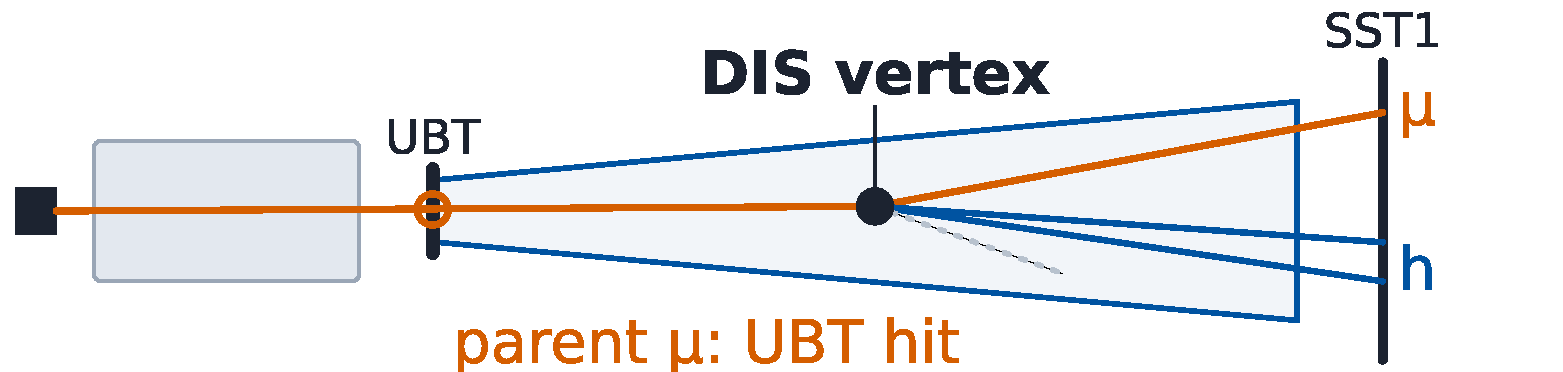
\includegraphics[width=1.00\linewidth,height=30pt,keepaspectratio]{figs/s15_sk1.pdf}\par}
\par}
\vspace{2.46pt}
{\fontsize{6.55pt}{6.92pt}\selectfont\setlength{\tabcolsep}{3.19pt}\renewcommand{\arraystretch}{1.42}
\begin{tabularx}{\linewidth}{>{\raggedright\arraybackslash}Xrrrrrr}
\textcolor{muted}{μ inelastic, per 15 years} & \textcolor{muted}{μ crossing (per spill)} & \textcolor{muted}{interactions} & \textcolor{muted}{≥ 2 good tracks} & \textcolor{muted}{pair cuts} & \textcolor{muted}{IP < 10 cm} & \textcolor{muted}{IP < 2.5 m} \\\headrule
helium & 8.4×10\textsuperscript{11} (5.6×10\textsuperscript{4}) & 1.3×10\textsuperscript{6} & (9.75 ± 0.04)×10\textsuperscript{4} & 8 830 ± 110 & 1 267 ± 40 & 8 740 ± 110 \\\rowrule
vessel walls & 8.4×10\textsuperscript{11} (5.6×10\textsuperscript{4}) & 2.2×10\textsuperscript{7} & (1.299 ± 0.005)×10\textsuperscript{6} & 1 680 ± 190 & 110 ± 49 & 1 460 ± 180 \\\rowrule
air around the vessel & 8.5×10\textsuperscript{11} (5.7×10\textsuperscript{4}) & 5.6×10\textsuperscript{6} & (2.29 ± 0.03)×10\textsuperscript{5} & 223 ± 79 & < 64 & 167 ± 68 \\\rowrule
air upstream of the vessel & 3.5×10\textsuperscript{11} (2.3×10\textsuperscript{4}) & 3.5×10\textsuperscript{5} & (1.381 ± 0.005)×10\textsuperscript{4} & 12.5 ± 1.5 & 1.2 ± 0.5 & 12.4 ± 1.5 \\\rowrule
UBT planes (material) & 5.8×10\textsuperscript{11} (3.9×10\textsuperscript{4}) & 3.1×10\textsuperscript{6} & (1.01 ± 0.01)×10\textsuperscript{5} & 2 030 ± 160 & 272 ± 59 & 2 030 ± 160 \\\rowrule
\end{tabularx}\par}
\vspace{2.46pt}
{\centering {\centering 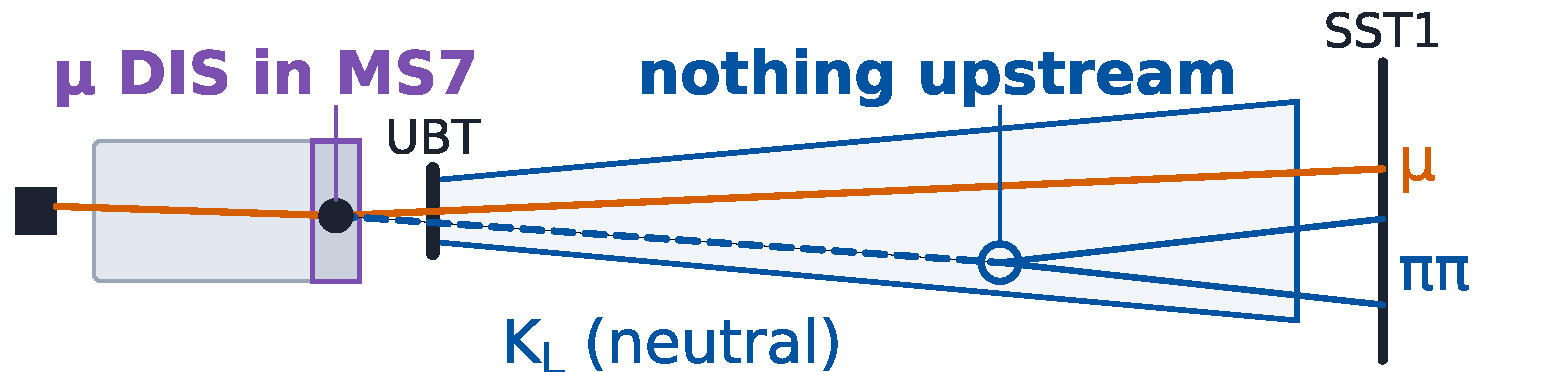
\includegraphics[width=1.00\linewidth,height=30pt,keepaspectratio]{figs/s15_sk2.pdf}\par}
\par}
\vspace{2.46pt}
{\fontsize{6.55pt}{6.92pt}\selectfont\setlength{\tabcolsep}{3.19pt}\renewcommand{\arraystretch}{1.42}
\begin{tabularx}{\linewidth}{>{\raggedright\arraybackslash}Xrrrrrr}
\textcolor{muted}{MS7 iron, last 50 cm, per 15 years} & \textcolor{muted}{μ crossing (per spill)} & \textcolor{muted}{interactions} & \textcolor{muted}{decays in vessel} & \textcolor{muted}{pair cuts} & \textcolor{muted}{IP < 10 cm} & \textcolor{muted}{IP < 2.5 m} \\\headrule
muons in the iron & 6.9×10\textsuperscript{15} (4.6×10\textsuperscript{8}) & 1.4×10\textsuperscript{13} & & & & \\\rowrule
K\textsubscript{L} & & & 3.0×10\textsuperscript{10} & 1.18×10\textsuperscript{7} & (1.27 ± 0.09)×10\textsuperscript{4} & (9.61 ± 0.05)×10\textsuperscript{6} \\\rowrule
K\textsuperscript{±} decaying in flight & & & 9.8×10\textsuperscript{10} & 2.3×10\textsuperscript{6} & (2.1 ± 0.9)×10\textsuperscript{3} & (1.86 ± 0.02)×10\textsuperscript{6} \\\rowrule
K\textsubscript{S}, Λ, Ξ\textsuperscript{0} & & & 1.3×10\textsuperscript{9} & 3 560 & 49 ± 49 & 3 560 \\\rowrule
\hline
\rowcolor{tint}\bfseries all & \bfseries  & \bfseries  & \bfseries  & \bfseries  & \bfseries (1.49 ± 0.13)×10\textsuperscript{4} & \bfseries (1.15 ± 0.01)×10\textsuperscript{7} \\\rowrule
\end{tabularx}\par}
\slidenote{MS7: P\textsubscript{int} = 2.0×10\textsuperscript{-3} per muon crossing the last 50 cm of iron (Kokoulin cross section, × 0.82 per nucleon in iron); “<”: no simulated event left, 90 \% CL upper limit 2.30 Σw\textsuperscript{2}/Σw.}
\begin{tikzpicture}[remember picture,overlay]
\node[anchor=north east,inner sep=0] (t1) at ([xshift=-14pt,yshift=-6pt]current page.north east) {
\includegraphics[width=125pt]{figs/talk_3.png}};
\node[anchor=north east,inner sep=0] at ([yshift=-2pt]t1.south east) {
\includegraphics[width=125pt]{figs/talk_4.png}};
\end{tikzpicture}
\end{btframe}

% ---------------------------------------------------------------- slide 17: Neutrino inelastic scattering: helium, walls, tagger planes and MS7
\begin{btframe}{4 · Backgrounds before tagging · ν inelastic}{Neutrino inelastic scattering: helium, walls, tagger planes and MS7}
{\centering {\centering 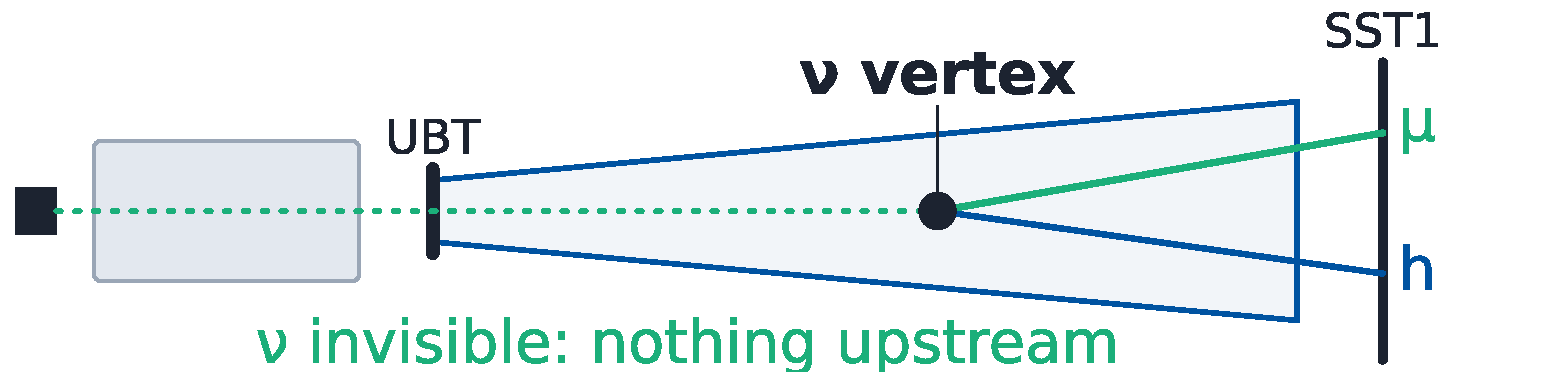
\includegraphics[width=1.00\linewidth,height=40.97pt,keepaspectratio]{figs/s16_sk1.pdf}\par}
\par}
\vspace{2.46pt}
{\fontsize{6.55pt}{7.83pt}\selectfont\setlength{\tabcolsep}{4.21pt}\renewcommand{\arraystretch}{1.42}
\begin{tabularx}{\linewidth}{>{\raggedright\arraybackslash}Xrrrrr}
\textcolor{muted}{ν inelastic, per 15 years} & \textcolor{muted}{interactions} & \textcolor{muted}{≥ 2 good tracks} & \textcolor{muted}{pair cuts} & \textcolor{muted}{IP < 10 cm} & \textcolor{muted}{IP < 2.5 m} \\\headrule
helium & 2.9×10\textsuperscript{4} & 3 231 ± 8 & 380 ± 2 & 3.1 ± 0.2 & 339 ± 2 \\\rowrule
vessel walls & 5.8×10\textsuperscript{4} & 1 581 ± 7 & 9.9 ± 0.5 & 0.02 ± 0.02 & 8.6 ± 0.4 \\\rowrule
air around & 5.0×10\textsuperscript{4} & 1 074 ± 7 & 0.6 ± 0.1 & < 0.04 & 0.5 ± 0.1 \\\rowrule
air upstream & 6518 & 176 ± 1 & 1.7 ± 0.1 & 0.04 ± 0.01 & 1.7 ± 0.1 \\\rowrule
UBT planes & 6.5×10\textsuperscript{4} & 1 287 ± 11 & 183 ± 4 & 2.7 ± 0.5 & 182 ± 4 \\\rowrule
MS7 iron & 2.0×10\textsuperscript{7} & (2.90 ± 0.04)×10\textsuperscript{5} & 820 ± 100 & 9.5 ± 6.5 & 800 ± 100 \\\rowrule
\hline
\rowcolor{tint}\bfseries total & \bfseries 2.0×10\textsuperscript{7} & \bfseries (2.98 ± 0.04)×10\textsuperscript{5} & \bfseries 1 400 & \bfseries 15 ± 7 & \bfseries 1 330 ± 100 \\\rowrule
\end{tabularx}\par}
\vspace{2.46pt}
{\centering {\centering 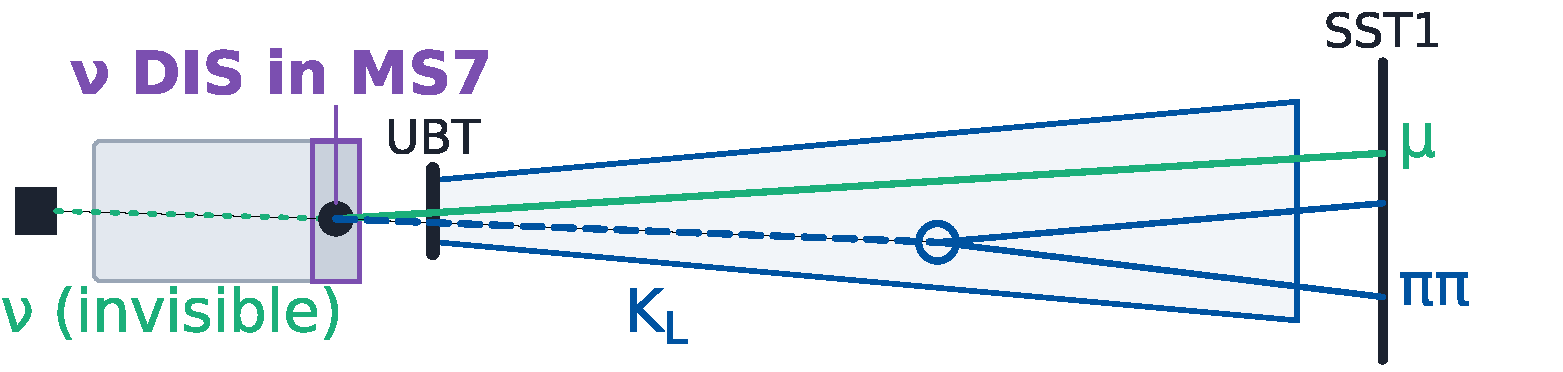
\includegraphics[width=1.00\linewidth,height=40.97pt,keepaspectratio]{figs/s16_sk2.pdf}\par}
\par}
\begin{tikzpicture}[remember picture,overlay]
\node[anchor=south west,inner sep=0] at ([xshift=14pt,yshift=26pt]current page.south west) {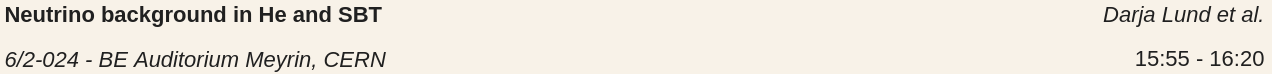
\includegraphics[width=140pt]{figs/talk_1.png}};
\end{tikzpicture}
\end{btframe}

% ---------------------------------------------------------------- slide 18: Combinatorial pairs: every cut, and all the pair types
\begin{btframe}{4 · Backgrounds before tagging · combinatorial}{Combinatorial pairs: every cut, and all the pair types}

{\centering 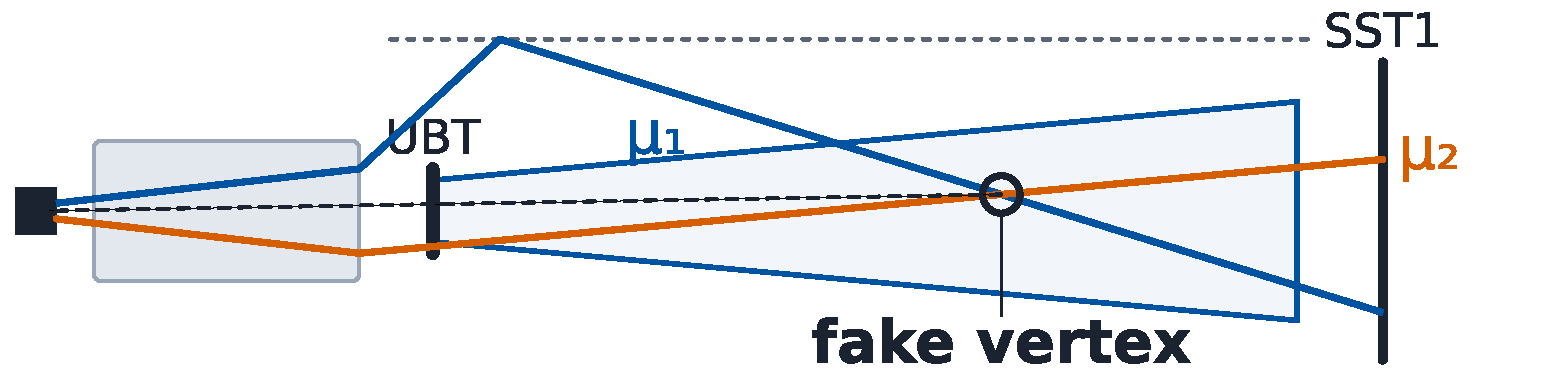
\includegraphics[width=1.00\linewidth,height=34.60pt,keepaspectratio]{figs/s17_sk1.pdf}\par}
\vspace{0.27pt}
{\centering \fontsize{6.01pt}{6.76pt}\selectfont μ × μ\par}
\par
\vspace{2.46pt}
{\fontsize{6.55pt}{7.83pt}\selectfont\setlength{\tabcolsep}{2.14pt}\renewcommand{\arraystretch}{1.42}
\begin{tabularx}{\linewidth}{l>{\raggedright\arraybackslash}Xrr}
\textcolor{muted}{cut} & \textcolor{muted}{} & \textcolor{muted}{per spill} & \textcolor{muted}{rejection} \\\headrule
track & in the SST1 acceptance & 3.19×10\textsuperscript{4} μ & – \\\rowrule
track & 4 straw stations + TD and p > 1 GeV (good tracks) & 6.3×10\textsuperscript{3} μ & ×5.0 \\\rowrule
pair & all pairs of good tracks in a spill & 2.1×10\textsuperscript{7} & – \\\rowrule
pair & opposite charge & 1.0×10\textsuperscript{7} & ×2.1 \\\rowrule
pair & DOCA < 1 cm & 1.9×10\textsuperscript{5} & ×54 \\\rowrule
pair & vertex 5 cm inside the vessel & 2 960 & ×63 \\\rowrule
pair & IP < 2.5 m (measured) & 2 310 & ×1.3 \\\rowrule
pair & IP < 10 cm (measured) & 121 & ×19 \\\rowrule
pair & time coincidence ±200 ps (× 4×10\textsuperscript{-10}) & 4.8×10\textsuperscript{-8} & ×2.5×10\textsuperscript{9} \\\rowrule
\rowcolor{tint}\bfseries 15 years & \bfseries × 1.5×10\textsuperscript{7} spills & \bfseries 0.73 (IP < 10 cm), 13.9 (IP < 2.5 m) & \bfseries  \\\rowrule
\end{tabularx}\par}
\vspace{2.46pt}

\end{btframe}

% ---------------------------------------------------------------- slide 19: combinatorial (2), restored 24 Nov 2026 with DOCA < 1 cm
\begin{btframe}{4 · Backgrounds before tagging · combinatorial (2)}{Combinatorial pairs: every cut, and all the pair types}
    
\begin{minipage}[t]{0.5\linewidth}
{\centering 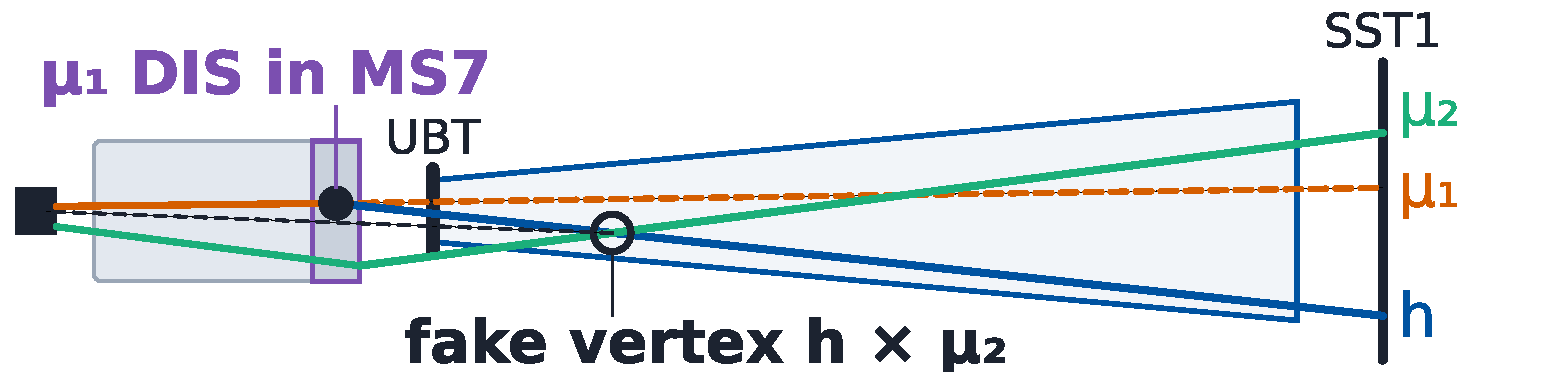
\includegraphics[width=1.00\linewidth,height=26pt,keepaspectratio]{figs/s17_sk2.pdf}\par}
\vspace{0.27pt}
{\centering \fontsize{6.01pt}{6.76pt}\selectfont μ × interaction product\par}
\end{minipage}%
\hfill%
\begin{minipage}[t]{0.5\linewidth}
{\centering 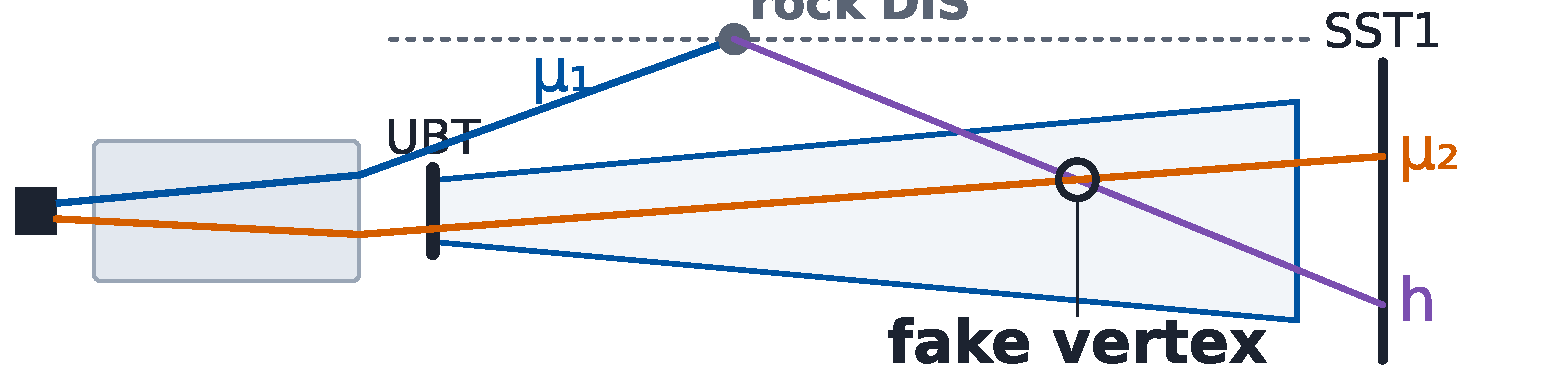
\includegraphics[width=1.00\linewidth,height=26pt,keepaspectratio]{figs/s17_sk3.pdf}\par}
\vspace{0.27pt}
{\centering \fontsize{5.01pt}{6.76pt}\selectfont μ × cavern-rock particle\par}
\end{minipage}
\vspace{2.46pt}
{\fontsize{6.2pt}{7.2pt}\selectfont\setlength{\tabcolsep}{2.14pt}\renewcommand{\arraystretch}{1.1}
\begin{tabularx}{\linewidth}{>{\raggedright\arraybackslash}Xrrr}
\textcolor{muted}{pairs per 15 years, ±200 ps, before tagging (DOCA < 1 cm; interactions with one track at SST1)} & \textcolor{muted}{pair cuts (no IP)} & \textcolor{muted}{IP < 10 cm} & \textcolor{muted}{IP < 2.5 m} \\\headrule
μ × μ & 14.3 & 0.73 & 13.9 \\\rowrule
\rowcolor{tint}\bfseries (MS7 μ interaction, 1 track) × μ & \bfseries 39.6 ± 1.4 & \bfseries 4.4 ± 0.3 & \bfseries 38.8 ± 1.4 \\\rowrule
(MS7 ν interaction, 1 track) × μ & 3.1×10\textsuperscript{-3} & 2.5×10\textsuperscript{-4} & 3.1×10\textsuperscript{-3} \\\rowrule
(vessel μ interaction, 1 track) × μ & 5.3×10\textsuperscript{-6} & 5×10\textsuperscript{-7} & 5.0×10\textsuperscript{-6} \\\rowrule
(vessel ν interaction, 1 track) × μ & 4.5×10\textsuperscript{-5} & 4.0×10\textsuperscript{-6} & 4.4×10\textsuperscript{-5} \\\rowrule
interaction × interaction (MS7 μ × MS7 μ) & 1.24 & 0.024 & 0.89 \\\rowrule
\rowcolor{tint}\bfseries (cavern-rock track) × μ &\bfseries  110 &\bfseries  42 &\bfseries  108 \\\rowrule
\rowcolor{tint}\bfseries total & \bfseries 165 & \bfseries 47 & \bfseries 162 \\\rowrule
\end{tabularx}\par}
\vspace{3pt}
{\centering 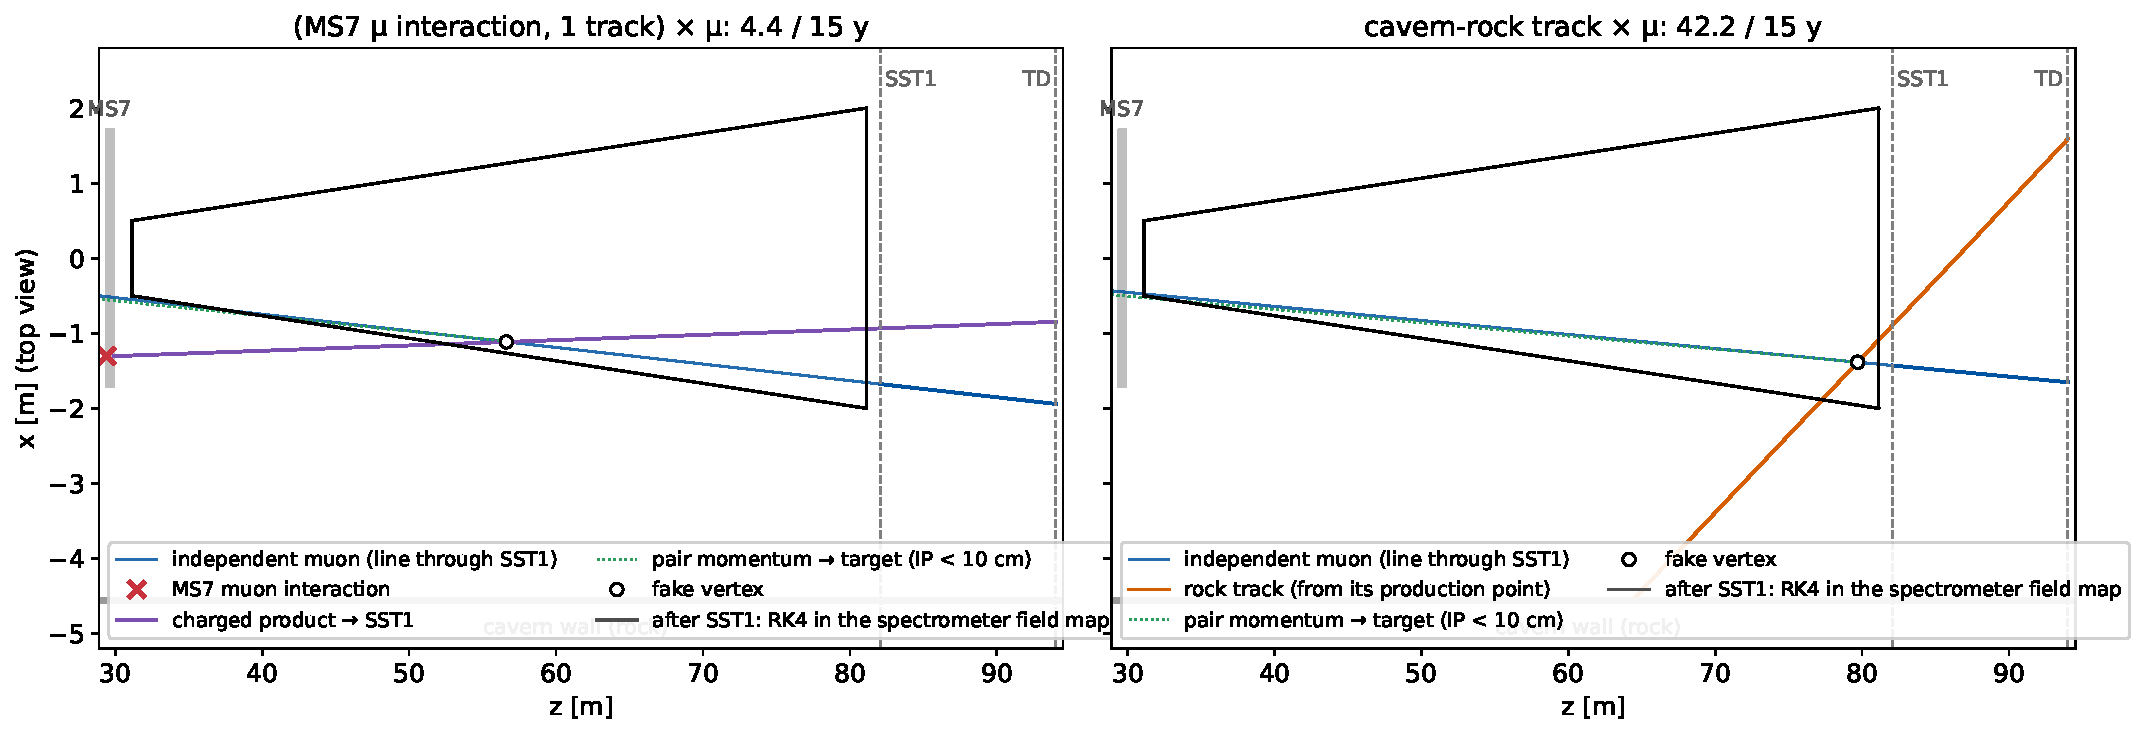
\includegraphics[width=0.92\linewidth,height=96pt,keepaspectratio]{figs/s20_pairs_tracks_doca1.pdf}\par}
\end{btframe}

% sections/04_background_tagging.tex: generated by newdeck/html2beamer.py from the HTML deck, then edited by hand

% ---------------------------------------------------------------- slide 19: Outline
\begin{btframe}{}{Outline}
\begin{outlinelist}
\outlineitem{1}{Introduction}{the background types, the geometry, the input muons and neutrinos}{0.35}
\outlineitem{2}{Simulation}{transport, inelastic scattering, technologies, hits and digitisation, signal generation}{0.35}
\outlineitem{3}{Selection}{track cuts, pair cuts and time coincidence}{0.35}
\outlineitem{4}{Backgrounds before tagging}{μ and ν inelastic scattering, MS7 K\textsubscript{L}, combinatorial pairs}{0.35}
\outlineitem{5}{Background tagging}{rules, V0 rule, SBT model, R1–R3, Z2–Z3, summary}{1.00}
\outlineitem{6}{Optimisation and conclusion}{genetic-algorithm search, the optimised design}{0.35}
\end{outlinelist}
\end{btframe}

% ---------------------------------------------------------------- slide 20: The reference designs R1, R2, R3
\begin{btframe}{5 · Background tagging · designs}{The reference designs R1, R2, R3}
\noindent \begin{minipage}[c]{40.97pt}\raggedright
{\fontsize{6.37pt}{8.60pt}\selectfont \textcolor{cern}{\textbf{R1}}\par}
\vspace{2.46pt}
{\fontsize{5.01pt}{6.76pt}\selectfont 99.7 drachmas\par}
\end{minipage}%
\hfill%
\begin{minipage}[c]{\dimexpr(1.0000\linewidth-1.0000\dimexpr46.09pt\relax)}\raggedright
{\centering {\renewcommand{\skubtlabel}{UBT: straws 1 × 2.7 m\textsuperscript{2} (4.8 dr) + tiles 4 × 4 m\textsuperscript{2}, 2 × 2 cm\textsuperscript{2} flames (94.8 dr)}\designsketch[52.35pt]{}{0}{}}\par}
\end{minipage}\par
\vspace{2.46pt}
\noindent \begin{minipage}[c]{40.97pt}\raggedright
{\fontsize{6.37pt}{8.60pt}\selectfont \textcolor{cern}{\textbf{R2}}\par}
\vspace{2.46pt}
{\fontsize{5.01pt}{6.76pt}\selectfont 333.5 drachmas = budget\newline{}\textcolor{purple}{+ V0 rule}\par}
\end{minipage}%
\hfill%
\begin{minipage}[c]{\dimexpr(1.0000\linewidth-1.0000\dimexpr46.09pt\relax)}\raggedright
{\centering {\renewcommand{\skubtlabel}{UBT: straws 1 × 2.7 m\textsuperscript{2} (4.8 dr) + tiles 4 × 4 m\textsuperscript{2}, 2 × 2 cm\textsuperscript{2} flames (94.8 dr)}\designsketch[52.35pt]{0,...,9}{0}{SBT: 854 LS cells, 20 cm, 10 rings (233.8 dr)}}\par}
\end{minipage}\par
\vspace{2.46pt}
\noindent \begin{minipage}[c]{40.97pt}\raggedright
{\fontsize{6.37pt}{8.60pt}\selectfont \textcolor{cern}{\textbf{R3}}\par}
\vspace{2.46pt}
{\fontsize{5.01pt}{6.76pt}\selectfont 378.7 drachmas\newline{}\textcolor{purple}{+ V0 rule}\par}
\end{minipage}%
\hfill%
\begin{minipage}[c]{\dimexpr(1.0000\linewidth-1.0000\dimexpr46.09pt\relax)}\raggedright
{\centering {\renewcommand{\skubtlabel}{UBT: straws 1 × 2.7 m\textsuperscript{2} (4.8 dr) + tiles 4 × 4 m\textsuperscript{2}, 2 × 2 cm\textsuperscript{2} flames (94.8 dr)}\renewcommand{\skmsmslabel}{MSMS: 24 Si stations\\30 × 30 cm\textsuperscript{2} (45.2 dr)}\designsketch[52.35pt]{0,...,9}{1}{SBT: 854 LS cells, 20 cm, 10 rings (233.8 dr)}}\par}
\end{minipage}\par
\end{btframe}

% ---------------------------------------------------------------- slide 21: How a candidate is tagged: tracks, neutrals, MS7
\begin{btframe}{5 · Background tagging · tagging chain}{How a candidate is tagged: tracks, neutrals, MS7}
{\fontsize{5.23pt}{7.07pt}\selectfont \textbf{Tracks: does a measured track come from upstream?}\par}
\vspace{2.46pt}
\begin{flowrow}{\dimexpr(\linewidth-3\dimexpr6.37pt\relax)/4\relax}{6.37pt}%
\flowstep{white}{rule}{2.28pt}{3.64pt}{{\fontsize{5.92pt}{7.40pt}\selectfont\textbf{\textcolor{cern}{candidate}}\par}\vspace{0.91pt}{\fontsize{5.01pt}{6.76pt}\selectfont\textcolor{ink}{2 tracks, vertex in the vessel}\par}}%
\flowarrow%
\flowstep{white}{rule}{2.28pt}{3.64pt}{{\fontsize{5.92pt}{7.40pt}\selectfont\textbf{\textcolor{cern}{each track back}}\par}\vspace{0.91pt}{\fontsize{5.01pt}{6.76pt}\selectfont\textcolor{ink}{straight line from SST1 to every plane upstream of the vertex}\par}}%
\flowarrow%
\flowstep{white}{rule}{2.28pt}{3.64pt}{{\fontsize{5.92pt}{7.40pt}\selectfont\textbf{\textcolor{cern}{window}}\par}\vspace{0.91pt}{\fontsize{5.01pt}{6.76pt}\selectfont\textcolor{ink}{r = 5 cm + (0.5 mrad + 6 mrad·GeV/p)·Δz, ±3σ in time; SBT along the wall}\par}}%
\flowarrow%
\flowstep{white}{rule}{2.28pt}{3.64pt}{{\fontsize{5.92pt}{7.40pt}\selectfont\textbf{\textcolor{cern}{hit?}}\par}\vspace{0.91pt}{\fontsize{5.01pt}{6.76pt}\selectfont\textcolor{ink}{yes → tagged (+ bounce search from the cavern wall)}\par}}%
\end{flowrow}
\vspace{2.46pt}
{\fontsize{5.23pt}{7.07pt}\selectfont \textcolor{purple}{\textbf{Neutrals (V0 rule, R2 and R3): was the candidate made upstream?}}\par}
\vspace{2.46pt}
\begin{flowrow}{\dimexpr(\linewidth-3\dimexpr6.37pt\relax)/4\relax}{6.37pt}%
\flowstep{white}{rule}{2.28pt}{3.64pt}{{\fontsize{5.92pt}{7.40pt}\selectfont\textbf{\textcolor{purple}{candidate}}\par}\vspace{0.91pt}{\fontsize{5.01pt}{6.76pt}\selectfont\textcolor{ink}{p\textsubscript{vis} = p\textsubscript{1} + p\textsubscript{2} < 20 GeV}\par}}%
\flowarrow%
\flowstep{white}{rule}{2.28pt}{3.64pt}{{\fontsize{5.92pt}{7.40pt}\selectfont\textbf{\textcolor{purple}{trace back as a neutral}}\par}\vspace{0.91pt}{\fontsize{5.01pt}{6.76pt}\selectfont\textcolor{ink}{from the vertex along p\textsubscript{vis} to the UBT}\par}}%
\flowarrow%
\flowstep{white}{rule}{2.28pt}{3.64pt}{{\fontsize{5.92pt}{7.40pt}\selectfont\textbf{\textcolor{purple}{disc + early window}}\par}\vspace{0.91pt}{\fontsize{5.01pt}{6.76pt}\selectfont\textcolor{ink}{r = 5 cm + max(25 mrad, 0.25 GeV/p\textsubscript{vis})·Δz; window opened by the K\textsubscript{L} flight time}\par}}%
\flowarrow%
\flowstep{white}{rule}{2.28pt}{3.64pt}{{\fontsize{5.92pt}{7.40pt}\selectfont\textbf{\textcolor{purple}{any hit?}}\par}\vspace{0.91pt}{\fontsize{5.01pt}{6.76pt}\selectfont\textcolor{ink}{yes → tagged: the parent muon or the other products}\par}}%
\end{flowrow}
\vspace{2.46pt}
{\fontsize{5.23pt}{7.07pt}\selectfont \textcolor{red}{\textbf{MS7 (MSMS, R3): did the interaction happen in the last iron?}}\par}
\vspace{2.46pt}
\begin{flowrow}{\dimexpr(\linewidth-3\dimexpr6.37pt\relax)/4\relax}{6.37pt}%
\flowstep{white}{rule}{2.28pt}{3.64pt}{{\fontsize{5.92pt}{7.40pt}\selectfont\textbf{\textcolor{red}{candidate}}\par}\vspace{0.91pt}{\fontsize{5.01pt}{6.76pt}\selectfont\textcolor{ink}{traced back as a neutral}\par}}%
\flowarrow%
\flowstep{white}{rule}{2.28pt}{3.64pt}{{\fontsize{5.92pt}{7.40pt}\selectfont\textbf{\textcolor{red}{strip layers}}\par}\vspace{0.91pt}{\fontsize{5.01pt}{6.76pt}\selectfont\textcolor{ink}{29.39 / 29.59 / 29.79 m, 24 stations}\par}}%
\flowarrow%
\flowstep{white}{rule}{2.28pt}{3.64pt}{{\fontsize{5.92pt}{7.40pt}\selectfont\textbf{\textcolor{red}{disc}}\par}\vspace{0.91pt}{\fontsize{5.01pt}{6.76pt}\selectfont\textcolor{ink}{2 cm + 10 mrad·Δz, ±1.5 ns}\par}}%
\flowarrow%
\flowstep{white}{rule}{2.28pt}{3.64pt}{{\fontsize{5.92pt}{7.40pt}\selectfont\textbf{\textcolor{red}{own products?}}\par}\vspace{0.91pt}{\fontsize{5.01pt}{6.76pt}\selectfont\textcolor{ink}{yes → tagged}\par}}%
\end{flowrow}
\slidenote{Source: veto lib/veto/reco.py v0\_tag (16–17 Nov 2026); numbers results\_rerun/reco/r123\_study\_v0statk\_1622cf7.json (bin/v0rule\_study.py, V0-enriched MS7 samples, full selection).}
\end{btframe}

% ---------------------------------------------------------------- slide 22: How a candidate is tagged: tracks
\begin{btframe}{5 · Background tagging · tagging chain 1/3}{How a candidate is tagged: tracks}
\noindent \begin{minipage}[c]{38.69pt}\raggedright
{\fontsize{4.32pt}{5.84pt}\selectfont \textcolor{cern}{\textbf{Tracks}}\par}
\end{minipage}%
\hfill%
\begin{minipage}[c]{\dimexpr(1.0000\linewidth-1.0000\dimexpr42.90pt\relax)}\raggedright
\begin{flowrow}{\dimexpr(\linewidth-3\dimexpr5.46pt\relax)/4\relax}{5.46pt}%
\flowstep{cern}{cern}{2.28pt}{3.64pt}{{\fontsize{4.78pt}{5.97pt}\selectfont\textbf{\textcolor{white}{candidate}}\par}\vspace{0.91pt}{\fontsize{4.10pt}{5.53pt}\selectfont\textcolor{white}{2 tracks, vertex in the vessel}\par}}%
\flowarrow%
\flowstep{cern}{cern}{2.28pt}{3.64pt}{{\fontsize{4.78pt}{5.97pt}\selectfont\textbf{\textcolor{white}{each track back}}\par}\vspace{0.91pt}{\fontsize{4.10pt}{5.53pt}\selectfont\textcolor{white}{straight line from SST1 upstream}\par}}%
\flowarrow%
\flowstep{cern}{cern}{2.28pt}{3.64pt}{{\fontsize{4.78pt}{5.97pt}\selectfont\textbf{\textcolor{white}{window}}\par}\vspace{0.91pt}{\fontsize{4.10pt}{5.53pt}\selectfont\textcolor{white}{r = 5 cm + (0.5 + 6 GeV/p) mrad·Δz, ±3σ}\par}}%
\flowarrow%
\flowstep{cern}{cern}{2.28pt}{3.64pt}{{\fontsize{4.78pt}{5.97pt}\selectfont\textbf{\textcolor{white}{hit?}}\par}\vspace{0.91pt}{\fontsize{4.10pt}{5.53pt}\selectfont\textcolor{white}{yes → tagged}\par}}%
\end{flowrow}
\end{minipage}\par
\vspace{2.46pt}
\fadeblock{0.28}{\noindent \begin{minipage}[c]{38.69pt}\raggedright
{\fontsize{4.32pt}{5.84pt}\selectfont \textcolor{purple}{\textbf{Neutrals (V0 rule, R2, R3)}}\par}
\end{minipage}%
\hfill%
\begin{minipage}[c]{\dimexpr(1.0000\linewidth-1.0000\dimexpr42.90pt\relax)}\raggedright
\begin{flowrow}{\dimexpr(\linewidth-3\dimexpr5.46pt\relax)/4\relax}{5.46pt}%
\flowstep{white}{rule}{2.28pt}{3.64pt}{{\fontsize{4.78pt}{5.97pt}\selectfont\textbf{\textcolor{purple}{candidate}}\par}\vspace{0.91pt}{\fontsize{4.10pt}{5.53pt}\selectfont\textcolor{ink}{p\textsubscript{vis} < 20 GeV}\par}}%
\flowarrow%
\flowstep{white}{rule}{2.28pt}{3.64pt}{{\fontsize{4.78pt}{5.97pt}\selectfont\textbf{\textcolor{purple}{trace back as a neutral}}\par}\vspace{0.91pt}{\fontsize{4.10pt}{5.53pt}\selectfont\textcolor{ink}{vertex → UBT along p\textsubscript{vis}}\par}}%
\flowarrow%
\flowstep{white}{rule}{2.28pt}{3.64pt}{{\fontsize{4.78pt}{5.97pt}\selectfont\textbf{\textcolor{purple}{disc + early window}}\par}\vspace{0.91pt}{\fontsize{4.10pt}{5.53pt}\selectfont\textcolor{ink}{5 cm + max(25, 250/p\textsubscript{vis}) mrad·Δz}\par}}%
\flowarrow%
\flowstep{white}{rule}{2.28pt}{3.64pt}{{\fontsize{4.78pt}{5.97pt}\selectfont\textbf{\textcolor{purple}{any hit?}}\par}\vspace{0.91pt}{\fontsize{4.10pt}{5.53pt}\selectfont\textcolor{ink}{yes → tagged}\par}}%
\end{flowrow}
\end{minipage}\par
}\vspace{2.46pt}
\fadeblock{0.28}{\noindent \begin{minipage}[c]{38.69pt}\raggedright
{\fontsize{4.32pt}{5.84pt}\selectfont \textcolor{red}{\textbf{MS7 (MSMS, R3)}}\par}
\end{minipage}%
\hfill%
\begin{minipage}[c]{\dimexpr(1.0000\linewidth-1.0000\dimexpr42.90pt\relax)}\raggedright
\begin{flowrow}{\dimexpr(\linewidth-3\dimexpr5.46pt\relax)/4\relax}{5.46pt}%
\flowstep{white}{rule}{2.28pt}{3.64pt}{{\fontsize{4.78pt}{5.97pt}\selectfont\textbf{\textcolor{red}{candidate}}\par}\vspace{0.91pt}{\fontsize{4.10pt}{5.53pt}\selectfont\textcolor{ink}{traced back as a neutral}\par}}%
\flowarrow%
\flowstep{white}{rule}{2.28pt}{3.64pt}{{\fontsize{4.78pt}{5.97pt}\selectfont\textbf{\textcolor{red}{strip layers}}\par}\vspace{0.91pt}{\fontsize{4.10pt}{5.53pt}\selectfont\textcolor{ink}{29.39 / 29.59 / 29.79 m}\par}}%
\flowarrow%
\flowstep{white}{rule}{2.28pt}{3.64pt}{{\fontsize{4.78pt}{5.97pt}\selectfont\textbf{\textcolor{red}{disc}}\par}\vspace{0.91pt}{\fontsize{4.10pt}{5.53pt}\selectfont\textcolor{ink}{2 cm + 10 mrad·Δz, ±1.5 ns}\par}}%
\flowarrow%
\flowstep{white}{rule}{2.28pt}{3.64pt}{{\fontsize{4.78pt}{5.97pt}\selectfont\textbf{\textcolor{red}{own products?}}\par}\vspace{0.91pt}{\fontsize{4.10pt}{5.53pt}\selectfont\textcolor{ink}{yes → tagged}\par}}%
\end{flowrow}
\end{minipage}\par
}\vspace{2.46pt}
\noindent \begin{minipage}[c]{\dimexpr(0.6000\linewidth-0.6000\dimexpr7.85pt\relax)}\raggedright
{\centering 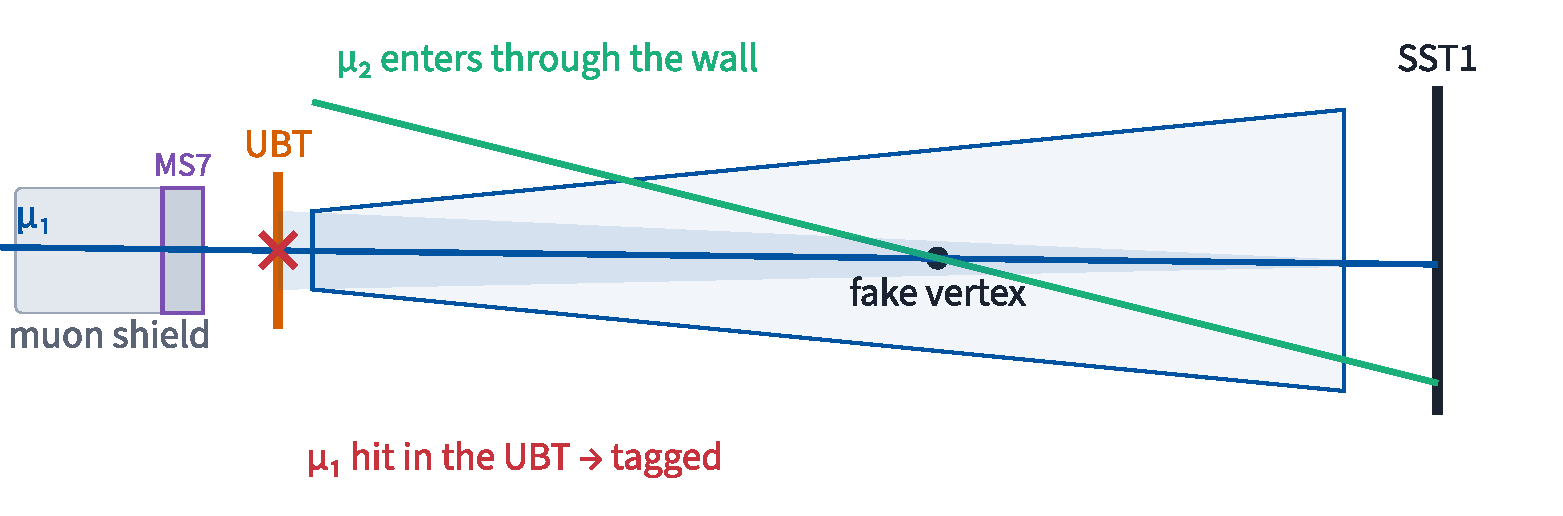
\includegraphics[width=1.00\linewidth,height=45.52pt,keepaspectratio]{figs/s21_sk1.pdf}\par}
\end{minipage}%
\hfill%
\begin{minipage}[c]{\dimexpr(0.4000\linewidth-0.4000\dimexpr7.85pt\relax)}\raggedright
\begin{mathbox}[cern]{5.23pt}
\textbf{window at each plane}\newline{}r = 5 cm + (0.5 mrad + 6 mrad·GeV / p) · Δz\newline{}|t\textsubscript{hit} − t\textsubscript{track}| < 3σ\textsubscript{t}\newline{}\textcolor{muted}{Δz: from SST1 back to the plane}\newline{}p = 10 GeV: r ≈ \textbf{11 cm}; p = 1 GeV: r ≈ \textbf{38 cm} at the UBT
\end{mathbox}
\end{minipage}\par
\vspace{2.46pt}
\noindent \begin{minipage}[c]{\dimexpr(0.6154\linewidth-0.6154\dimexpr7.85pt\relax)}\raggedright
{\centering 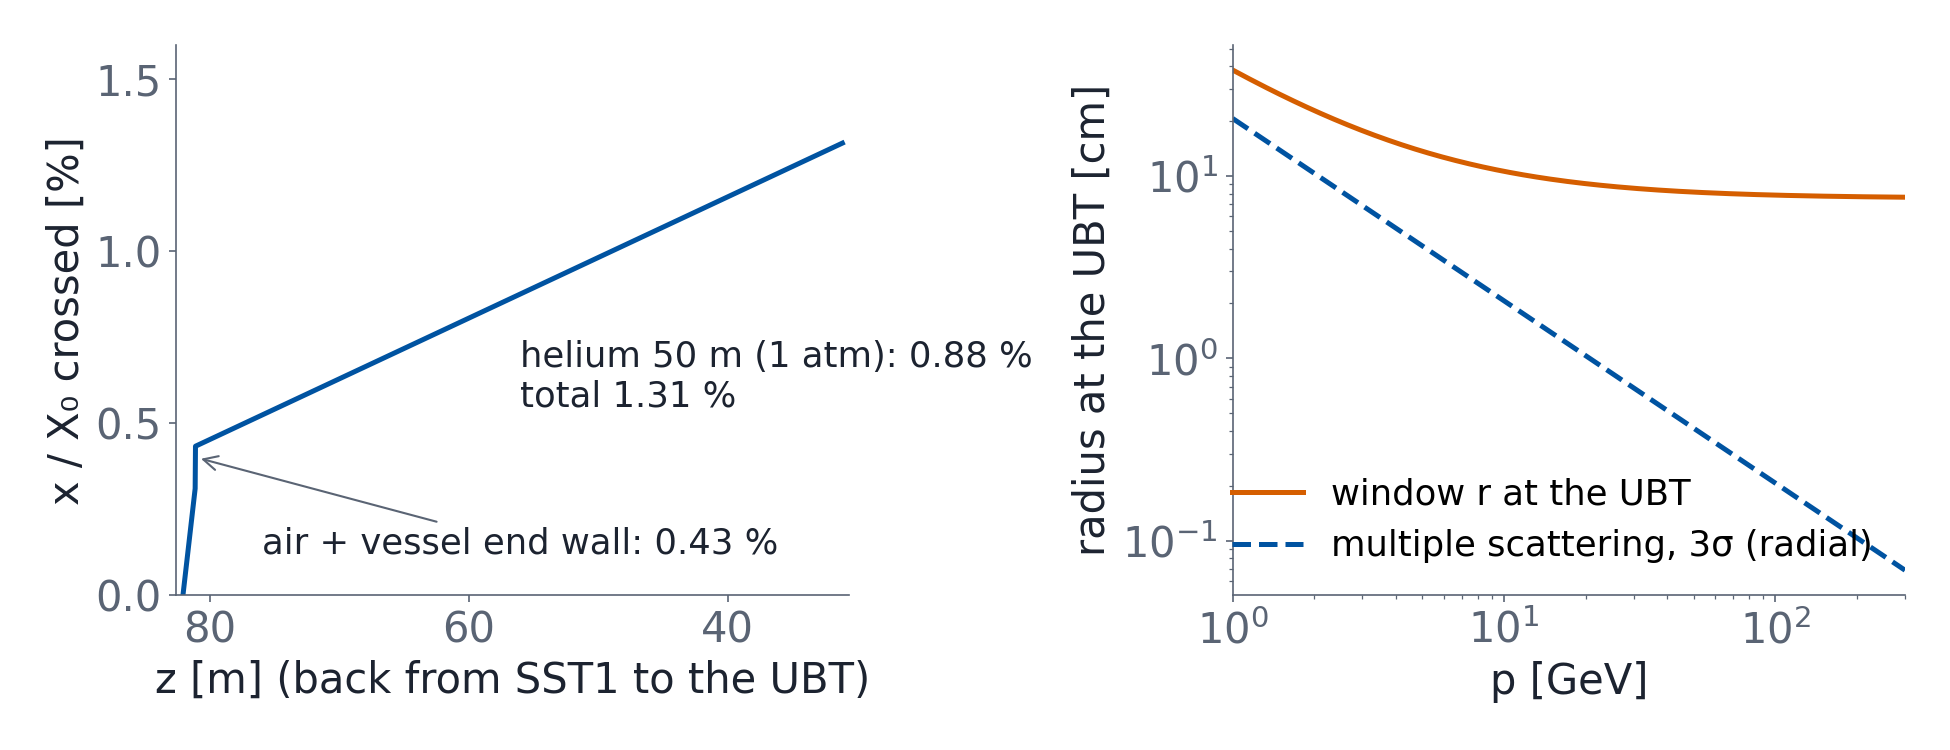
\includegraphics[height=72.83pt,keepaspectratio]{figs/s21_img2.png}\par}
\end{minipage}%
\hfill%
\begin{minipage}[c]{\dimexpr(0.3846\linewidth-0.3846\dimexpr7.85pt\relax)}\raggedright
{\fontsize{4.55pt}{6.15pt}\selectfont Back from SST1 to the UBT a track crosses \textbf{1.3 \% X\textsubscript{0}} (air, vessel end wall, 50 m of helium). Its multiple scattering (Highland, 3σ) stays inside the window at every momentum: \textbf{21 cm vs 38 cm} at 1 GeV. A hit in the window and ±3σ in time → \textbf{tagged}.\par}
\end{minipage}\par
\end{btframe}

% ---------------------------------------------------------------- slide 23: How a candidate is tagged: neutrals (V0 rule)
\begin{btframe}{5 · Background tagging · tagging chain 2/3}{How a candidate is tagged: neutrals (V0 rule)}
\fadeblock{0.28}{\noindent \begin{minipage}[c]{38.69pt}\raggedright
{\fontsize{4.32pt}{5.84pt}\selectfont \textcolor{cern}{\textbf{Tracks}}\par}
\end{minipage}%
\hfill%
\begin{minipage}[c]{\dimexpr(1.0000\linewidth-1.0000\dimexpr42.90pt\relax)}\raggedright
\begin{flowrow}{\dimexpr(\linewidth-3\dimexpr5.46pt\relax)/4\relax}{5.46pt}%
\flowstep{white}{rule}{2.28pt}{3.64pt}{{\fontsize{4.78pt}{5.97pt}\selectfont\textbf{\textcolor{cern}{candidate}}\par}\vspace{0.91pt}{\fontsize{4.10pt}{5.53pt}\selectfont\textcolor{ink}{2 tracks, vertex in the vessel}\par}}%
\flowarrow%
\flowstep{white}{rule}{2.28pt}{3.64pt}{{\fontsize{4.78pt}{5.97pt}\selectfont\textbf{\textcolor{cern}{each track back}}\par}\vspace{0.91pt}{\fontsize{4.10pt}{5.53pt}\selectfont\textcolor{ink}{straight line from SST1 upstream}\par}}%
\flowarrow%
\flowstep{white}{rule}{2.28pt}{3.64pt}{{\fontsize{4.78pt}{5.97pt}\selectfont\textbf{\textcolor{cern}{window}}\par}\vspace{0.91pt}{\fontsize{4.10pt}{5.53pt}\selectfont\textcolor{ink}{r = 5 cm + (0.5 + 6 GeV/p) mrad·Δz, ±3σ}\par}}%
\flowarrow%
\flowstep{white}{rule}{2.28pt}{3.64pt}{{\fontsize{4.78pt}{5.97pt}\selectfont\textbf{\textcolor{cern}{hit?}}\par}\vspace{0.91pt}{\fontsize{4.10pt}{5.53pt}\selectfont\textcolor{ink}{yes → tagged}\par}}%
\end{flowrow}
\end{minipage}\par
}\vspace{2.46pt}
\noindent \begin{minipage}[c]{38.69pt}\raggedright
{\fontsize{4.32pt}{5.84pt}\selectfont \textcolor{purple}{\textbf{Neutrals (V0 rule, R2, R3)}}\par}
\end{minipage}%
\hfill%
\begin{minipage}[c]{\dimexpr(1.0000\linewidth-1.0000\dimexpr42.90pt\relax)}\raggedright
\begin{flowrow}{\dimexpr(\linewidth-3\dimexpr5.46pt\relax)/4\relax}{5.46pt}%
\flowstep{purple}{purple}{2.28pt}{3.64pt}{{\fontsize{4.78pt}{5.97pt}\selectfont\textbf{\textcolor{white}{candidate}}\par}\vspace{0.91pt}{\fontsize{4.10pt}{5.53pt}\selectfont\textcolor{white}{p\textsubscript{vis} < 20 GeV}\par}}%
\flowarrow%
\flowstep{purple}{purple}{2.28pt}{3.64pt}{{\fontsize{4.78pt}{5.97pt}\selectfont\textbf{\textcolor{white}{trace back as a neutral}}\par}\vspace{0.91pt}{\fontsize{4.10pt}{5.53pt}\selectfont\textcolor{white}{vertex → UBT along p\textsubscript{vis}}\par}}%
\flowarrow%
\flowstep{purple}{purple}{2.28pt}{3.64pt}{{\fontsize{4.78pt}{5.97pt}\selectfont\textbf{\textcolor{white}{disc + early window}}\par}\vspace{0.91pt}{\fontsize{4.10pt}{5.53pt}\selectfont\textcolor{white}{5 cm + max(25, 250/p\textsubscript{vis}) mrad·Δz}\par}}%
\flowarrow%
\flowstep{purple}{purple}{2.28pt}{3.64pt}{{\fontsize{4.78pt}{5.97pt}\selectfont\textbf{\textcolor{white}{any hit?}}\par}\vspace{0.91pt}{\fontsize{4.10pt}{5.53pt}\selectfont\textcolor{white}{yes → tagged}\par}}%
\end{flowrow}
\end{minipage}\par
\vspace{2.46pt}
\fadeblock{0.28}{\noindent \begin{minipage}[c]{38.69pt}\raggedright
{\fontsize{4.32pt}{5.84pt}\selectfont \textcolor{red}{\textbf{MS7 (MSMS, R3)}}\par}
\end{minipage}%
\hfill%
\begin{minipage}[c]{\dimexpr(1.0000\linewidth-1.0000\dimexpr42.90pt\relax)}\raggedright
\begin{flowrow}{\dimexpr(\linewidth-3\dimexpr5.46pt\relax)/4\relax}{5.46pt}%
\flowstep{white}{rule}{2.28pt}{3.64pt}{{\fontsize{4.78pt}{5.97pt}\selectfont\textbf{\textcolor{red}{candidate}}\par}\vspace{0.91pt}{\fontsize{4.10pt}{5.53pt}\selectfont\textcolor{ink}{traced back as a neutral}\par}}%
\flowarrow%
\flowstep{white}{rule}{2.28pt}{3.64pt}{{\fontsize{4.78pt}{5.97pt}\selectfont\textbf{\textcolor{red}{strip layers}}\par}\vspace{0.91pt}{\fontsize{4.10pt}{5.53pt}\selectfont\textcolor{ink}{29.39 / 29.59 / 29.79 m}\par}}%
\flowarrow%
\flowstep{white}{rule}{2.28pt}{3.64pt}{{\fontsize{4.78pt}{5.97pt}\selectfont\textbf{\textcolor{red}{disc}}\par}\vspace{0.91pt}{\fontsize{4.10pt}{5.53pt}\selectfont\textcolor{ink}{2 cm + 10 mrad·Δz, ±1.5 ns}\par}}%
\flowarrow%
\flowstep{white}{rule}{2.28pt}{3.64pt}{{\fontsize{4.78pt}{5.97pt}\selectfont\textbf{\textcolor{red}{own products?}}\par}\vspace{0.91pt}{\fontsize{4.10pt}{5.53pt}\selectfont\textcolor{ink}{yes → tagged}\par}}%
\end{flowrow}
\end{minipage}\par
}\vspace{2.46pt}
\noindent \begin{minipage}[c]{\dimexpr(0.6000\linewidth-0.6000\dimexpr7.85pt\relax)}\raggedright
{\centering 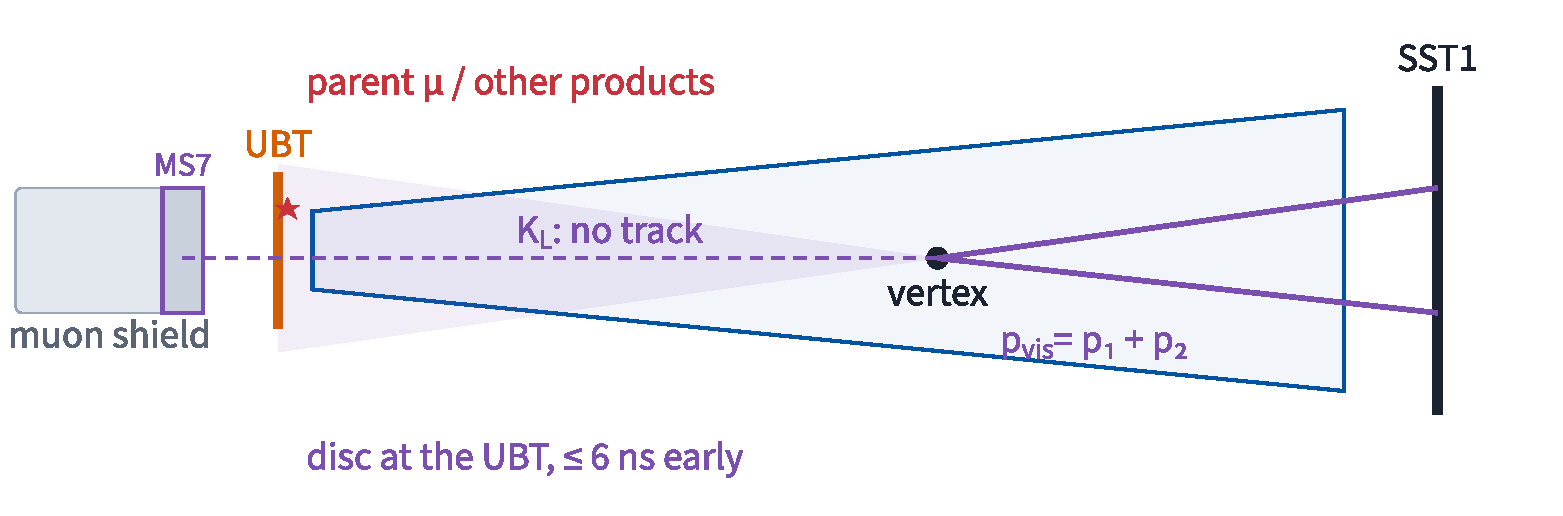
\includegraphics[width=1.00\linewidth,height=59.18pt,keepaspectratio]{figs/s22_sk1.pdf}\par}
\end{minipage}%
\hfill%
\begin{minipage}[c]{\dimexpr(0.4000\linewidth-0.4000\dimexpr7.85pt\relax)}\raggedright
\begin{mathbox}[purple]{5.23pt}
\textbf{neutral back-trace}\newline{}r = 5 cm + max(25 mrad, 0.25 GeV / p\textsubscript{vis}) · Δz\newline{}−w − t\textsubscript{early} < Δt < w, t\textsubscript{early} ≤ 6 ns\newline{}\textcolor{muted}{Δz: from the vertex back to the plane}
\end{mathbox}
\end{minipage}\par
\vspace{2.46pt}
{\fontsize{4.55pt}{6.37pt}\selectfont
\begin{itemize}
  \item A K\textsubscript{L} made upstream leaves no track: only its decay pair is seen
  \item Trace back from the vertex along p\textsubscript{vis}: vertex at 50 m → UBT, Δz ≈ 19 m\newline{}p\textsubscript{vis} = 15 GeV: θ = 25 mrad, r = 5 cm + 25 mrad × 19 m ≈ \textbf{0.5 m}\newline{}p\textsubscript{vis} = 5 GeV: θ = 50 mrad, r ≈ \textbf{1.0 m}
  \item The K\textsubscript{L} is slow: the window opens up to its flight time earlier (≤ 6 ns). Any hit (parent muon, sister particles) → \textbf{tagged}
\end{itemize}}
\end{btframe}

% ---------------------------------------------------------------- slide 24: How a candidate is tagged: MS7 strips
\begin{btframe}{5 · Background tagging · tagging chain 3/3}{How a candidate is tagged: MS7 strips}
\fadeblock{0.28}{\noindent \begin{minipage}[c]{38.69pt}\raggedright
{\fontsize{4.32pt}{5.84pt}\selectfont \textcolor{cern}{\textbf{Tracks}}\par}
\end{minipage}%
\hfill%
\begin{minipage}[c]{\dimexpr(1.0000\linewidth-1.0000\dimexpr42.90pt\relax)}\raggedright
\begin{flowrow}{\dimexpr(\linewidth-3\dimexpr5.46pt\relax)/4\relax}{5.46pt}%
\flowstep{white}{rule}{2.28pt}{3.64pt}{{\fontsize{4.78pt}{5.97pt}\selectfont\textbf{\textcolor{cern}{candidate}}\par}\vspace{0.91pt}{\fontsize{4.10pt}{5.53pt}\selectfont\textcolor{ink}{2 tracks, vertex in the vessel}\par}}%
\flowarrow%
\flowstep{white}{rule}{2.28pt}{3.64pt}{{\fontsize{4.78pt}{5.97pt}\selectfont\textbf{\textcolor{cern}{each track back}}\par}\vspace{0.91pt}{\fontsize{4.10pt}{5.53pt}\selectfont\textcolor{ink}{straight line from SST1 upstream}\par}}%
\flowarrow%
\flowstep{white}{rule}{2.28pt}{3.64pt}{{\fontsize{4.78pt}{5.97pt}\selectfont\textbf{\textcolor{cern}{window}}\par}\vspace{0.91pt}{\fontsize{4.10pt}{5.53pt}\selectfont\textcolor{ink}{r = 5 cm + (0.5 + 6 GeV/p) mrad·Δz, ±3σ}\par}}%
\flowarrow%
\flowstep{white}{rule}{2.28pt}{3.64pt}{{\fontsize{4.78pt}{5.97pt}\selectfont\textbf{\textcolor{cern}{hit?}}\par}\vspace{0.91pt}{\fontsize{4.10pt}{5.53pt}\selectfont\textcolor{ink}{yes → tagged}\par}}%
\end{flowrow}
\end{minipage}\par
}\vspace{2.46pt}
\fadeblock{0.28}{\noindent \begin{minipage}[c]{38.69pt}\raggedright
{\fontsize{4.32pt}{5.84pt}\selectfont \textcolor{purple}{\textbf{Neutrals (V0 rule, R2, R3)}}\par}
\end{minipage}%
\hfill%
\begin{minipage}[c]{\dimexpr(1.0000\linewidth-1.0000\dimexpr42.90pt\relax)}\raggedright
\begin{flowrow}{\dimexpr(\linewidth-3\dimexpr5.46pt\relax)/4\relax}{5.46pt}%
\flowstep{white}{rule}{2.28pt}{3.64pt}{{\fontsize{4.78pt}{5.97pt}\selectfont\textbf{\textcolor{purple}{candidate}}\par}\vspace{0.91pt}{\fontsize{4.10pt}{5.53pt}\selectfont\textcolor{ink}{p\textsubscript{vis} < 20 GeV}\par}}%
\flowarrow%
\flowstep{white}{rule}{2.28pt}{3.64pt}{{\fontsize{4.78pt}{5.97pt}\selectfont\textbf{\textcolor{purple}{trace back as a neutral}}\par}\vspace{0.91pt}{\fontsize{4.10pt}{5.53pt}\selectfont\textcolor{ink}{vertex → UBT along p\textsubscript{vis}}\par}}%
\flowarrow%
\flowstep{white}{rule}{2.28pt}{3.64pt}{{\fontsize{4.78pt}{5.97pt}\selectfont\textbf{\textcolor{purple}{disc + early window}}\par}\vspace{0.91pt}{\fontsize{4.10pt}{5.53pt}\selectfont\textcolor{ink}{5 cm + max(25, 250/p\textsubscript{vis}) mrad·Δz}\par}}%
\flowarrow%
\flowstep{white}{rule}{2.28pt}{3.64pt}{{\fontsize{4.78pt}{5.97pt}\selectfont\textbf{\textcolor{purple}{any hit?}}\par}\vspace{0.91pt}{\fontsize{4.10pt}{5.53pt}\selectfont\textcolor{ink}{yes → tagged}\par}}%
\end{flowrow}
\end{minipage}\par
}\vspace{2.46pt}
\noindent \begin{minipage}[c]{38.69pt}\raggedright
{\fontsize{4.32pt}{5.84pt}\selectfont \textcolor{red}{\textbf{MS7 (MSMS, R3)}}\par}
\end{minipage}%
\hfill%
\begin{minipage}[c]{\dimexpr(1.0000\linewidth-1.0000\dimexpr42.90pt\relax)}\raggedright
\begin{flowrow}{\dimexpr(\linewidth-3\dimexpr5.46pt\relax)/4\relax}{5.46pt}%
\flowstep{red}{red}{2.28pt}{3.64pt}{{\fontsize{4.78pt}{5.97pt}\selectfont\textbf{\textcolor{white}{candidate}}\par}\vspace{0.91pt}{\fontsize{4.10pt}{5.53pt}\selectfont\textcolor{white}{traced back as a neutral}\par}}%
\flowarrow%
\flowstep{red}{red}{2.28pt}{3.64pt}{{\fontsize{4.78pt}{5.97pt}\selectfont\textbf{\textcolor{white}{strip layers}}\par}\vspace{0.91pt}{\fontsize{4.10pt}{5.53pt}\selectfont\textcolor{white}{29.39 / 29.59 / 29.79 m}\par}}%
\flowarrow%
\flowstep{red}{red}{2.28pt}{3.64pt}{{\fontsize{4.78pt}{5.97pt}\selectfont\textbf{\textcolor{white}{disc}}\par}\vspace{0.91pt}{\fontsize{4.10pt}{5.53pt}\selectfont\textcolor{white}{2 cm + 10 mrad·Δz, ±1.5 ns}\par}}%
\flowarrow%
\flowstep{red}{red}{2.28pt}{3.64pt}{{\fontsize{4.78pt}{5.97pt}\selectfont\textbf{\textcolor{white}{own products?}}\par}\vspace{0.91pt}{\fontsize{4.10pt}{5.53pt}\selectfont\textcolor{white}{yes → tagged}\par}}%
\end{flowrow}
\end{minipage}\par
\vspace{2.46pt}
\noindent \begin{minipage}[c]{\dimexpr(0.6000\linewidth-0.6000\dimexpr7.85pt\relax)}\raggedright
{\centering 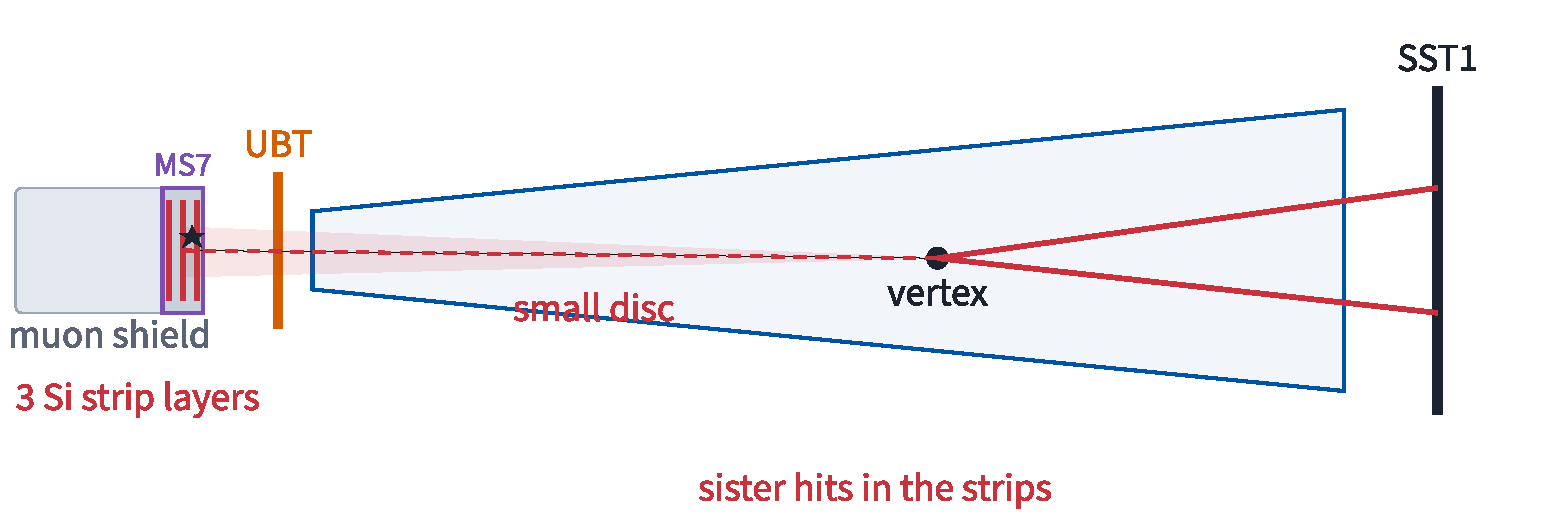
\includegraphics[width=1.00\linewidth,height=59.18pt,keepaspectratio]{figs/s23_sk1.pdf}\par}
\end{minipage}%
\hfill%
\begin{minipage}[c]{\dimexpr(0.4000\linewidth-0.4000\dimexpr7.85pt\relax)}\raggedright
\begin{mathbox}[red]{5.23pt}
\textbf{strip disc}\newline{}r = 2 cm + 10 mrad · Δz\newline{}|Δt| < 1.5 ns\newline{}\textcolor{muted}{Δz: from the vertex back to the strip layer}
\end{mathbox}
\end{minipage}\par
\vspace{2.46pt}
{\fontsize{4.55pt}{6.37pt}\selectfont
\begin{itemize}
  \item K\textsubscript{L} made in the last iron (MS7) by the muon: the parent muon and other products cross the strips
  \item Same back-trace, but the strips are close and precise: vertex at 50 m → MS7 (29.6 m), Δz ≈ 20 m\newline{}r = 2 cm + 10 mrad × 20 m ≈ \textbf{22 cm}, ±1.5 ns
  \item Own products in the disc → \textbf{tagged}. At full selection the V0 rule alone already leaves 0.67 ± 0.32 MS7 events (R2 = R3); the strips help the partial selection: 4.7×10\textsuperscript{4} → 3.6×10\textsuperscript{4}
  \item Applied to \textbf{every} candidate: the origin is not assumed. A candidate not made in MS7 has no strip hits on its line, except by chance (that is the random-hit cost)
\end{itemize}}
\end{btframe}

% ---------------------------------------------------------------- slide 25: Slow MS7 KL escaped the 25 mrad cone: three fixes, A + C adopted
\begin{btframe}{5 · Background tagging · V0 rule fixes}{Slow MS7 K\textsubscript{L} escaped the 25 mrad cone: three fixes, A + C adopted}
\noindent \begin{minipage}[t]{\dimexpr(0.2500\linewidth-0.2500\dimexpr14.22pt\relax)}\vspace{0pt}\raggedright
{\centering \fontsize{4.55pt}{6.15pt}\selectfont \textcolor{purple}{\textbf{25 mrad cone: misses (slow K\textsubscript{L})}}\par}
\vspace{0.27pt}
{\centering 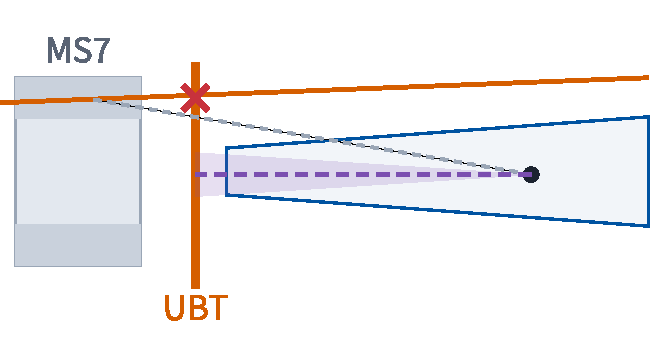
\includegraphics[width=1.00\linewidth,height=63.73pt,keepaspectratio]{figs/s24_sk1.pdf}\par}
\end{minipage}%
\hfill%
\begin{minipage}[t]{\dimexpr(0.2500\linewidth-0.2500\dimexpr14.22pt\relax)}\vspace{0pt}\raggedright
{\centering \fontsize{4.55pt}{6.15pt}\selectfont \textcolor{purple}{\textbf{A: cone max(25 mrad, 0.25 GeV / p\textsubscript{vis})}}\par}
\vspace{0.27pt}
{\centering 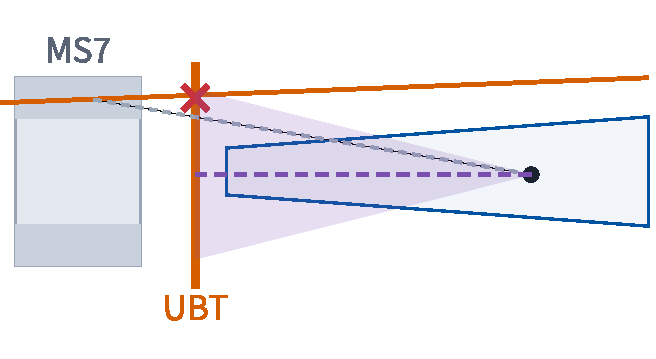
\includegraphics[width=1.00\linewidth,height=63.73pt,keepaspectratio]{figs/s24_sk2.pdf}\par}
\end{minipage}%
\hfill%
\begin{minipage}[t]{\dimexpr(0.2500\linewidth-0.2500\dimexpr14.22pt\relax)}\vspace{0pt}\raggedright
{\centering \fontsize{4.55pt}{6.15pt}\selectfont \textcolor{purple}{\textbf{B: extra lines to the yoke legs}}\par}
\vspace{0.27pt}
{\centering 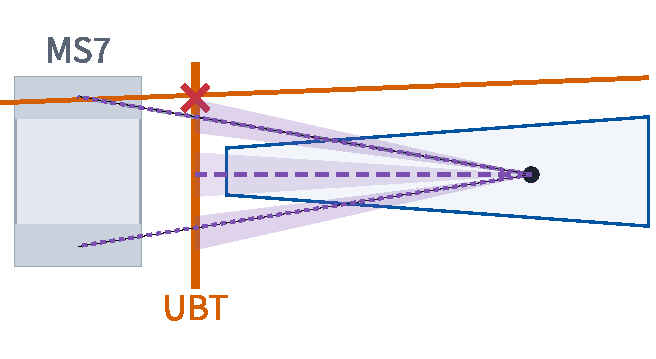
\includegraphics[width=1.00\linewidth,height=63.73pt,keepaspectratio]{figs/s24_sk3.pdf}\par}
\end{minipage}%
\hfill%
\begin{minipage}[t]{\dimexpr(0.2500\linewidth-0.2500\dimexpr14.22pt\relax)}\vspace{0pt}\raggedright
{\centering \fontsize{4.55pt}{6.15pt}\selectfont \textcolor{purple}{\textbf{C: window opened by the K\textsubscript{L} flight time}}\par}
\vspace{0.27pt}
{\centering 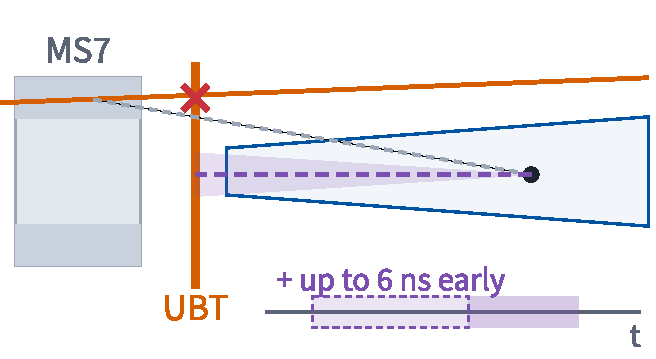
\includegraphics[width=1.00\linewidth,height=63.73pt,keepaspectratio]{figs/s24_sk4.pdf}\par}
\end{minipage}\par
\vspace{2.46pt}
{\fontsize{4.37pt}{5.68pt}\selectfont\setlength{\tabcolsep}{3.06pt}\renewcommand{\arraystretch}{1.42}
\begin{tabularx}{\linewidth}{>{\raggedright\arraybackslash}Xrrrr}
\textcolor{muted}{variant} & \textcolor{muted}{signal lost F / P} & \textcolor{muted}{MS7 μ tagged} & \textcolor{muted}{own hits only} & \textcolor{muted}{MS7 μ left / 15 y} \\\headrule
R3 with 25 mrad & 5.3 / 9.4 \% & 66 \% & 63 \% & 8.1×10\textsuperscript{3} \\\rowrule
A: 1/p cone & 5.4 / 10.5 \% & 100 \% & 100 \% & 0.63 \\\rowrule
B: yoke lines & 12.1 / 25.1 \% & 100 \% & 100 \% & 0.48 \\\rowrule
C: time of flight & 4.9 / 7.6 \% & 68 \% & 67 \% & 7.8×10\textsuperscript{3} \\\rowrule
\rowcolor{tint}\bfseries A + C (adopted, R3) & \bfseries 5.0 / 8.4 \% & \bfseries 100 \% & \bfseries 100 \% & \bfseries 0.67 \\\rowrule
B + C & 11.5 / 21.8 \% & 100 \% & 100 \% & 0.48 \\\rowrule
\end{tabularx}\par}
\slidenote{Source: results\_rerun/r3\_escapes/variants/v0study\_variants.json and v0study\_variants\_ownhits.json (bin/v0rule\_study.py, code 2e228bf); signal: results\_rerun/reco/r3var\_*.json (bin/run\_reco.py). Before the D19 energy loss and SBT ×4.}
\end{btframe}

% ---------------------------------------------------------------- slide 26: The SBT model: material, rules, energy loss, random rate
\begin{btframe}{5 · Background tagging · SBT model}{The SBT model: material, rules, energy loss, random rate}
{\fontsize{4.74pt}{6.16pt}\selectfont\setlength{\tabcolsep}{3.32pt}\renewcommand{\arraystretch}{1.42}
\begin{tabularx}{\linewidth}{l>{\raggedright\arraybackslash}Xr}
\textcolor{muted}{ingredient} & \textcolor{muted}{what} & \textcolor{muted}{effect (R2)} \\\headrule
SBT material as a target (Al / LS / ribs) & 1.2×10\textsuperscript{4} μ-induced candidates / 15 y (IP < 10 cm) & new background class \\\rowrule
v0\_line + self-tag & own LS deposits of the interaction & 783 → 113 (SBT rules alone) \\\rowrule
zone rule & in-time cell downstream of the vertex & ν in helium 3.5 → 1.1; signal −0.6 \% (×1) / −2.3 \% (×4) \\\rowrule
scattering in the shell (k = 1) & kick at the exit of each shell piece & single μ tagging 92 → 85 \% \\\rowrule
mean energy loss in the shell & Al 0.436, LS 0.150 GeV/m; soft muons stop & 45 \% of single-μ weight stops; tagging → 95 \%; pairs 2.36 → 1.14 \\\rowrule
random rate ×4 & cavern back-scatter, e / γ (SR-389: ×13) & signal +2 points (zone rule) \\\rowrule
\end{tabularx}\par}
\slidenote{Source: veto docs/d19\_sbt.md sections 4–8, ISSUES D19 (closed 17 Nov); results\_rerun/sbt\_d19/flags17/ and sbt\_d19/rangeout/summary\_R2.json (bin/sbt\_eval.py, bin/run\_reco.py; Slurm 2112324).}
\end{btframe}

% ---------------------------------------------------------------- slide 27: R1: UBT only — 99.7 drachmas, 18 100 channels
\begin{btframe}{5 · Background tagging · R1}{R1: UBT only — 99.7 drachmas, 18 100 channels}
{\centering \designsketch[54.62pt]{}{0}{}\par}
\vspace{2.46pt}
\noindent \begin{minipage}[t]{\dimexpr(0.5556\linewidth-0.5556\dimexpr11.49pt\relax)}\vspace{0pt}\raggedright
{\fontsize{5.31pt}{6.90pt}\selectfont\setlength{\tabcolsep}{3.72pt}\renewcommand{\arraystretch}{1.42}
\begin{tabular}{lr}
\textcolor{muted}{per 15 y, full selection} & \textcolor{muted}{R1} \\\headrule
signal lost, full / partial IP cut & 2.45 / 2.24 \% (4.0 / 3.8 at UBT rate ×2) \\\rowrule
μμ pairs & < 0.26 (90 \% CL) \\\rowrule
rock × μ pairs & 0.59 ± 0.09 \\\rowrule
interaction product × μ pairs & 0.019 ± 0.002 \\\rowrule
μ in the vessel & 70 ± 8 \\\rowrule
ν in the vessel & 3.5 \\\rowrule
MS7 μ (V0, K\textsuperscript{±}) & 1.70×10\textsuperscript{4} \\\rowrule
ν in MS7 & 2.6 \\\rowrule
\end{tabular}\par}
\end{minipage}%
\hfill%
\begin{minipage}[t]{\dimexpr(0.4444\linewidth-0.4444\dimexpr11.49pt\relax)}\vspace{0pt}\raggedright
{\fontsize{6.15pt}{8.60pt}\selectfont
\begin{itemize}
  \item Straws on the window + 4 × 4 m\textsuperscript{2} tile plane (2 × 2 cm\textsuperscript{2} in the flames)
  \item Catches what enters through the entrance window; blind to the side walls (rock tracks, bounced muons)
  \item Signal loss: 1.5 points EM debris on the straws, 1 point muons in the flame tiles
\end{itemize}}
\end{minipage}\par
\slidenote{Source: results\_rerun/reco/reco\_R1\_ubt\_only\_\{full,partial\}\_base0eb5209[\_ubtx2].json (bin/run\_reco.py), r123\_ms7\_base0eb5209.json (bin/v0rule\_study.py, MS7), r123\_vessel\_d19\_d3065c3.json (vessel μ/ν, bin/vessel\_prepare.py caches), sbt\_d19/rangeout/summary\_*.json, rock\_comb\_*\_ul90\_0030e68.json; code 0eb5209.}
\end{btframe}

% ---------------------------------------------------------------- slide 28: R2: SBT + UBT + V0 rule — 333.5 drachmas (the budget), 31 764 channels
\begin{btframe}{5 · Background tagging · R2}{R2: SBT + UBT + V0 rule — 333.5 drachmas (the budget), 31 764 channels}
{\centering \designsketch[54.62pt]{0,...,9}{0}{SBT: 10 rings, 854 liquid-scintillator cells on the four walls}\par}
\vspace{2.46pt}
\noindent \begin{minipage}[t]{\dimexpr(0.5556\linewidth-0.5556\dimexpr11.49pt\relax)}\vspace{0pt}\raggedright
{\fontsize{5.31pt}{6.90pt}\selectfont\setlength{\tabcolsep}{3.72pt}\renewcommand{\arraystretch}{1.42}
\begin{tabular}{lr}
\textcolor{muted}{per 15 y, full selection} & \textcolor{muted}{R2} \\\headrule
signal lost, full / partial IP cut & 6.7 / 9.7 \% (9.3 / 14.1 at UBT rate ×2) \\\rowrule
μμ pairs & < 0.052 (90 \% CL) \\\rowrule
rock × μ pairs & < 0.018 (90 \% CL) \\\rowrule
interaction product × μ pairs & < 1.1×10\textsuperscript{-4} \\\rowrule
μ in the vessel & 1.3 ± 1.3 (1 event) \\\rowrule
ν in the vessel & 1.09 ± 0.10 \\\rowrule
SBT material μ / ν & 0 (K\textsubscript{L} < 13) / 0.05 \\\rowrule
\rowcolor{tint}\bfseries MS7 μ (V0, K\textsuperscript{±}) & \bfseries 0.67 ± 0.32 \\\rowrule
ν in MS7 & 0.70 \\\rowrule
\end{tabular}\par}
\end{minipage}%
\hfill%
\begin{minipage}[t]{\dimexpr(0.4444\linewidth-0.4444\dimexpr11.49pt\relax)}\vspace{0pt}\raggedright
{\fontsize{6.15pt}{8.60pt}\selectfont
\begin{itemize}
  \item Removes everything entering through the walls: pairs, rock, vessel μ
  \item Single SST1 muons tagged 95 \%
  \item \textbf{V0 rule} (A+C, software only): MS7 1.8×10\textsuperscript{4} → \textbf{0.67}, SBT-material K\textsubscript{L} 112 → < 13
  \item Cost of the V0 rule: signal 5.0 / 5.2 → 6.7 / 9.7 \%
\end{itemize}}
\end{minipage}\par
\slidenote{Source: R2 with the V0 rule (designs/R2\_sbt\_ubt.json detector.v0\_rule, 18 Nov 2026; Slurm 2125101): results\_rerun/reco/reco\_R2\_sbt\_ubt\_\{full,partial\}\_r2v0[\_ubtx2].json (bin/run\_reco.py), r2v0\_ms7.json, r2v0\_vessel\_d19.json (bin/v0rule\_study.py), sbt\_d19/rangeout\_r2v0/summary\_R2.json (bin/sbt\_eval.py, bin/sbt\_summary.py), rock\_comb\_R2\_sbt\_ubt\_r2v0.json.}
\end{btframe}

% ---------------------------------------------------------------- slide 29: R3: R2 + Muon Shield Monitoring System — 378.7 drachmas
\begin{btframe}{5 · Background tagging · R3}{R3: R2 + Muon Shield Monitoring System — 378.7 drachmas}
{\centering \designsketch[45.52pt]{0,...,9}{1}{SBT: 10 rings, 854 liquid-scintillator cells on the four walls}\par}
\vspace{2.46pt}
\noindent \begin{minipage}[t]{\dimexpr(0.5405\linewidth-0.5405\dimexpr11.49pt\relax)}\vspace{0pt}\raggedright
{\fontsize{5.31pt}{6.90pt}\selectfont\setlength{\tabcolsep}{3.72pt}\renewcommand{\arraystretch}{1.42}
\begin{tabular}{lr}
\textcolor{muted}{per 15 y, full selection} & \textcolor{muted}{R3} \\\headrule
signal lost, full / partial IP cut & 6.8 / 10.2 \% (9.2 / 14.9 at UBT rate ×2) \\\rowrule
μμ, rock × μ pairs & < 0.052, < 0.018 \\\rowrule
interaction product × μ pairs & < 1.1×10\textsuperscript{-4} (≤ R2) \\\rowrule
μ in the vessel & 1.3 ± 1.3 (1 event) \\\rowrule
ν in the vessel & 1.09 ± 0.10 \\\rowrule
SBT material μ / ν & 0 (K\textsubscript{L} < 13) / 0.05 \\\rowrule
\rowcolor{tint}\bfseries MS7 μ (V0, K\textsuperscript{±}) & \bfseries 0.7 ± 0.3 \\\rowrule
ν in MS7 & 0.70 \\\rowrule
\end{tabular}\par}
\end{minipage}%
\hfill%
\begin{minipage}[t]{\dimexpr(0.4595\linewidth-0.4595\dimexpr11.49pt\relax)}\vspace{0pt}\raggedright
{\fontsize{6.15pt}{8.60pt}\selectfont
\begin{itemize}
  \item \textbf{Why MSMS:} the MS7 K\textsubscript{L} are the largest background and neutral; the only handle is the interaction itself, inside the last iron: 3 × 8 strip stations (30 × 30 cm\textsuperscript{2}) on the return-yoke legs, 82 \% of the V0 interaction points
  \item On top of R2 (with the V0 rule) the strips change nothing at full selection; partial selection MS7 4.7×10\textsuperscript{4} → 3.6×10\textsuperscript{4}
  \item +45 drachmas over the budget
\end{itemize}}
\end{minipage}\par
\slidenote{Source: results\_rerun/reco/reco\_R3\_sbt\_ubt\_strips\_\{full,partial\}\_base0eb5209[\_ubtx2].json (bin/run\_reco.py), r123\_ms7\_base0eb5209.json (bin/v0rule\_study.py, MS7), r123\_vessel\_d19\_d3065c3.json (vessel μ/ν, bin/vessel\_prepare.py caches), sbt\_d19/rangeout/summary\_*.json, rock\_comb\_*\_ul90\_0030e68.json; code 0eb5209.}
\end{btframe}

% ---------------------------------------------------------------- slide 30: R1, R2, R3: background left in 15 years and signal lost
\begin{btframe}{5 · Background tagging · summary}{R1, R2, R3: background left in 15 years and signal lost}
{\fontsize{5.31pt}{6.90pt}\selectfont\setlength{\tabcolsep}{3.72pt}\renewcommand{\arraystretch}{1.42}
\begin{tabularx}{\linewidth}{>{\raggedright\arraybackslash}Xrrr}
\textcolor{muted}{per 15 y, full selection} & \textcolor{muted}{R1} & \textcolor{muted}{R2} & \textcolor{muted}{R3} \\\headrule
μμ pairs & < 0.26 & < 0.052 & < 0.052 \\\rowrule
rock × μ pairs & 0.59 & < 0.018 & < 0.018 \\\rowrule
interaction product × μ pairs & 0.019 & < 1.1×10\textsuperscript{-4} & < 1.1×10\textsuperscript{-4} \\\rowrule
μ in the vessel (helium, walls) & 70 & 1.3 (1 ev.) & 1.3 (1 ev.) \\\rowrule
SBT material, K\textsubscript{L} / other & – & < 13 / < 940 & < 13 / < 940 \\\rowrule
MS7 μ (V0, K\textsuperscript{±}) & 1.70×10\textsuperscript{4} & 0.67 ± 0.32 & 0.7 ± 0.3 \\\rowrule
ν in the vessel & 3.5 & 1.09 & 1.09 \\\rowrule
ν in MS7 / SBT material & 2.6 / – & 0.70 / 0.05 & 0.70 / 0.05 \\\rowrule
\rowcolor{tint}\bfseries signal lost, full / partial IP cut & \bfseries 2.45 / 2.24 \% & \bfseries 6.74 / 9.71 \% & \bfseries 6.83 / 10.16 \% \\\rowrule
\rowcolor{tint}\bfseries signal lost at UBT rate ×2 & \bfseries 3.98 / 3.83 \% & \bfseries 9.33 / 14.14 \% & \bfseries 9.17 / 14.88 \% \\\rowrule
\end{tabularx}\par}
\vspace{2.46pt}
{\fontsize{6.15pt}{8.60pt}\selectfont
\begin{itemize}
  \item “<”: no simulated event left, 90 \% CL upper limit 2.30 Σw\textsuperscript{2}/Σw
  \item With the V0 rule, R2 leaves the same background as R3: the MSMS strips only help the partial selection
  \item Signal is lost only to random hits in the search windows: the V0 disc is the most sensitive (+2.6 / +4.4 points at twice the UBT rate)
\end{itemize}}
\slidenote{Source: R1, R3 report Table 7 (tab:tag:eff), code 0eb5209; R2 with the V0 rule: the *\_r2v0 files (Slurm 2125101); signal at UBT ×2: reco\_R*\_\{full,partial\}\_base0eb5209\_ubtx2.json (bin/run\_reco.py --plane-rate-scale 2). Interactions in the tagger planes themselves (350 μ, 3.4 ν before tagging) not yet included.}
\end{btframe}

% ---------------------------------------------------------------- slide 31: Z2: R2 without the SBT, 7 straw fins per side — 439.7 drachmas, 193 368 channels
\begin{btframe}{5 · Background tagging · Z2}{Z2 (optimised): SBT 6 rings + UBT + V0 rule — 225.3 drachmas, 21 171 channels}
{\centering {\renewcommand{\skubtlabel}{UBT: straws + tiles |x| < 1.7 m, 2 × 2 cm\textsuperscript{2} only on the cavern side}\designsketch[45.52pt]{2,5,6,7,8,9}{0}{SBT: rings 2, 5–9 (6 of 10)}}\par}
\vspace{2.46pt}
\noindent \begin{minipage}[t]{\dimexpr(0.5556\linewidth-0.5556\dimexpr11.49pt\relax)}\vspace{0pt}\raggedright
{\fontsize{5.31pt}{6.90pt}\selectfont\setlength{\tabcolsep}{3.72pt}\renewcommand{\arraystretch}{1.42}
\begin{tabular}{lr}
\textcolor{muted}{per 15 y, full selection} & \textcolor{muted}{Z2} \\\headrule
signal lost, full IP cut & 2.71 \% \\\rowrule
combinatorial pairs & 0 simulated pairs left \\\rowrule
μ in the vessel & 1.3 ± 1.3 (1 event) \\\rowrule
ν in the helium & 1.13 ± 0.11 \\\rowrule
SBT material & 0.004 ± 0.003 \\\rowrule
\rowcolor{tint}\bfseries MS7 (μ V0, K\textsuperscript{±}, ν) & \bfseries 0.80 ± 0.34 \\\rowrule
single SST1 muons tagged, all / bounced & 91 / 84 \% \\\rowrule
\end{tabular}\par}
\end{minipage}%
\hfill%
\begin{minipage}[t]{\dimexpr(0.4444\linewidth-0.4444\dimexpr11.49pt\relax)}\vspace{0pt}\raggedright
{\fontsize{6.15pt}{8.60pt}\selectfont
\begin{itemize}
  \item Best design of the genetic-algorithm search (section 6): R2 with 6 of the 10 SBT rings (no 0, 1, 3, 4)
  \item UBT straws with t\textsubscript{0} and the segment cut; tile plane |x| < 1.7 m, 2×2 cm only on the cavern side
  \item V0 rule with a 15.7 mrad cone, no K\textsubscript{L} time-of-flight window, p\textsubscript{max} kept
  \item \textbf{Signal loss 2.7 \%} (R2: 6.7 \%), 68 \% of the budget; every plane within its rate limit
\end{itemize}}
\end{minipage}\par
\slidenote{Optimised design (ga7c3 of run results\_rerun/evolve/ga\_20261119\_115533, re-scored −71.0 ± 0.5 over 3 seeds); design file results\_rerun/evolve/Z2\_opt\_ga7c3.json. Evaluated with the optimiser chain (full selection, UBT rate ×1). The vessel μ is the single helium event of R2; the SBT-material gain over the seed is one heavy event.}
\end{btframe}

% ---------------------------------------------------------------- slide 32: Z3 (optimised)
\begin{btframe}{5 · Background tagging · Z3}{Z3 (optimised): SBT 7 rings + UBT + V0 rule — 244.7 drachmas, 22 428 channels}
{\centering {\renewcommand{\skubtlabel}{UBT: straws + tiles |x| < 1.7 m, 2 × 2 cm\textsuperscript{2} only on the cavern side}\designsketch[45.52pt]{2,3,5,6,7,8,9}{0}{SBT: rings 2, 3, 5–9 (7 of 10)}}\par}
\vspace{2.46pt}
\noindent \begin{minipage}[t]{\dimexpr(0.5556\linewidth-0.5556\dimexpr11.49pt\relax)}\vspace{0pt}\raggedright
{\fontsize{5.31pt}{6.90pt}\selectfont\setlength{\tabcolsep}{3.72pt}\renewcommand{\arraystretch}{1.42}
\begin{tabular}{lr}
\textcolor{muted}{per 15 y, full selection} & \textcolor{muted}{Z3} \\\headrule
signal lost, full IP cut & 3.01 \% \\\rowrule
combinatorial pairs & 0 simulated pairs left \\\rowrule
μ in the vessel & 1.3 ± 1.3 (1 event) \\\rowrule
ν in the helium & 1.05 ± 0.10 \\\rowrule
SBT material & 0.004 ± 0.003 \\\rowrule
\rowcolor{tint}\bfseries MS7 (μ V0, K\textsuperscript{±}, ν) & \bfseries 0.61 ± 0.27 \\\rowrule
single SST1 muons tagged, all / bounced & 94 / 84 \% \\\rowrule
\end{tabular}\par}
\end{minipage}%
\hfill%
\begin{minipage}[t]{\dimexpr(0.4444\linewidth-0.4444\dimexpr11.49pt\relax)}\vspace{0pt}\raggedright
{\fontsize{6.15pt}{8.60pt}\selectfont
\begin{itemize}
  \item Second design of the search: as Z2 with ring 3 back (7 rings)
  \item MS7 0.61 and single SST1 tagging 94 \% (Z2: 0.80, 91 \%) for +19 drachmas
  \item \textbf{Signal loss 3.0 \%}, 73 \% of the budget
\end{itemize}}
\end{minipage}\par
\slidenote{Optimised design (ga8c8 of run results\_rerun/evolve/ga\_20261119\_115533, re-scored −75.9 ± 5.9 over 3 seeds); design file results\_rerun/evolve/Z3\_opt\_ga8c8.json. Evaluated with the optimiser chain (full selection, UBT rate ×1).}
\end{btframe}

% ---------------------------------------------------------------- slide 33: What R2 and R3 leave, and what is not yet known
\begin{btframe}{5 · Background tagging · what is left}{What R2 and R3 leave, and what is not yet known}
{\fontsize{6.15pt}{8.60pt}\selectfont
\begin{itemize}
  \item \textbf{Neutrinos in the helium} (1.1 / 15 y): no charged particle upstream; the zone rule removes two thirds
  \item \textbf{Neutrinos in MS7} (0.7 / 15 y)
  \item \textbf{Statistics}: μμ pairs < 0.05, vessel walls < 49, SBT non-K\textsubscript{L} < 940 per 15 y at 90 \% CL: not yet shown to be below 0.1; enriched samples needed
\end{itemize}}
\slidenote{Source: results\_rerun/closure/mu\_he\_survivor.json (bin/mu\_he\_survivor\_diag.py on prepared\_muon\_nov4full\_d19); 90 \% CL limits from the sample weights (veto interactions.ul90, code 0030e68).}
\end{btframe}

% sections/05_next_steps.tex: generated by newdeck/html2beamer.py from the HTML deck, then edited by hand
% ---------------------------------------------------------------- slide 34: Outline
\begin{btframe}{}{Outline}
\begin{outlinelist}
\outlineitem{1}{Introduction}{the background types, the geometry, the input muons and neutrinos}{0.35}
\outlineitem{2}{Simulation}{transport, inelastic scattering, technologies, hits and digitisation, signal generation}{0.35}
\outlineitem{3}{Selection}{track cuts, pair cuts and time coincidence}{0.35}
\outlineitem{4}{Backgrounds before tagging}{μ and ν inelastic scattering, MS7 K\textsubscript{L}, combinatorial pairs}{0.35}
\outlineitem{5}{Background tagging}{rules, V0 rule, SBT model, R1, R2, summary}{0.35}
\outlineitem{6}{Optimisation and conclusion}{genetic-algorithm search, the optimised design Z1}{1.00}
\end{outlinelist}
\end{btframe}




% ---------------------------------------------------------------- slide 35: design optimisation with a genetic algorithm (19 Nov 2026)
\begin{btframe}{6 · Optimisation · method}{Design optimisation: a genetic algorithm on the full chain}
\begin{minipage}[t]{0.56\linewidth}\vspace{0pt}
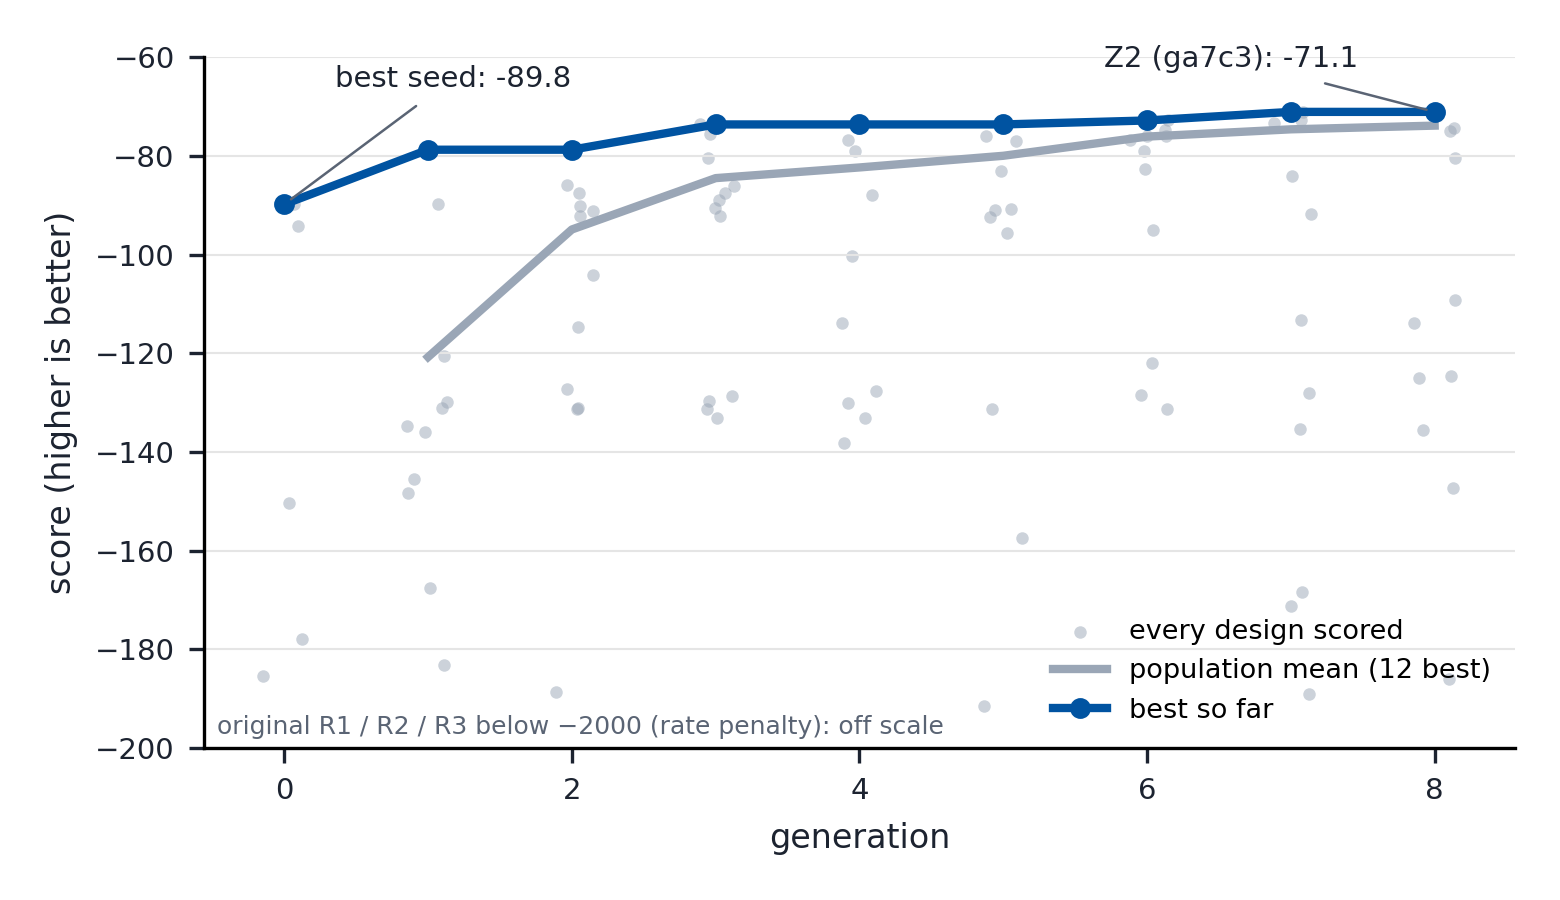
\includegraphics[width=\linewidth]{figs/s35_ga_convergence.png}
\end{minipage}\hfill
\begin{minipage}[t]{0.41\linewidth}\vspace{2pt}

\begin{figure}
    \centering
    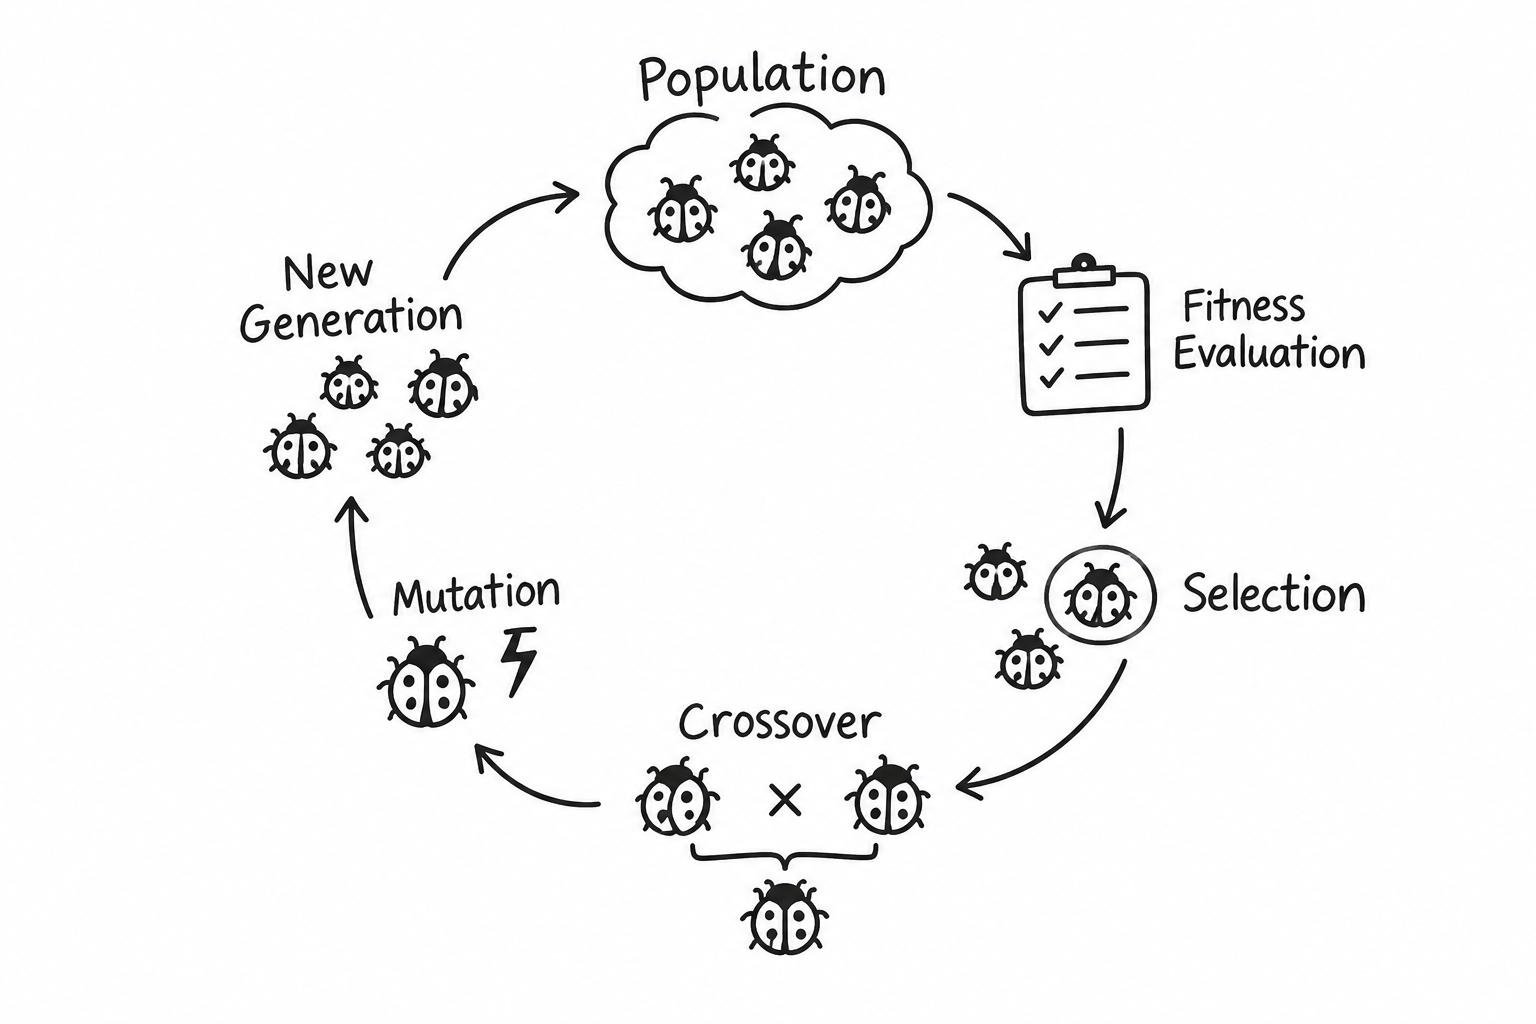
\includegraphics[width=1\linewidth]{figs/GA.png}
\end{figure}
\end{minipage}

{\fontsize{6.15pt}{8.60pt}\selectfont
\begin{itemize}
  \item \textbf{Genes}: SBT rings and threshold, UBT straw extent, tile plane size and 2×2 / 4×4 cm regions, V0 rule settings
  \item \textbf{Each generation}: 12 children by crossover + mutation, scored on Slurm with the chain of this talk (10\textsuperscript{5} signal decays); keep the 12 best
  \item \textbf{Score}: background left, signal lost, cost, rate limits; and the untagged fraction of bounced single SST1 muons
  \item \textbf{Seeds}: the reference designs and R1 / R2 with a 3.4 m tile plane, 2×2 cm only in the cavern-side flame block
  \item Model fixed; V0 p\textsubscript{max} cut held on
\end{itemize}}

\end{btframe}




% ---------------------------------------------------------------- slide 31: Z1: R2 without the SBT, 7 straw fins per side — 439.7 drachmas, 193 368 channels
\begin{btframe}{6 · Optimisation · Z1}{Z1 (optimised): SBT 6 rings + UBT + V0 rule — 225.3 drachmas, 21 171 channels}
{\centering {\renewcommand{\skubtlabel}{UBT: straws + tiles |x| < 1.7 m, 2 × 2 cm\textsuperscript{2} only on the cavern side}\designsketch[74.52pt]{2,5,6,7,8,9}{0}{SBT: rings 2, 5–9 (6 of 10)}}\par}
\vspace{2.46pt}
\noindent \begin{minipage}[c]{0.5\linewidth}
{\fontsize{5.31pt}{6.90pt}\selectfont\setlength{\tabcolsep}{3.72pt}\renewcommand{\arraystretch}{1.42}
\begin{tabular}{lr}
\textcolor{muted}{per 15 y, full selection} & \textcolor{muted}{Z1} \\\headrule
signal lost, full / partial IP cut & 2.79 / 2.43 \% \\\rowrule
μμ pairs & < 0.11 (90 \% CL) \\\rowrule
rock × μ pairs & (1.2 ± 0.9)×10\textsuperscript{-5} \\\rowrule
interaction product × μ pairs & 0.0012 ± 0.0002 \\\rowrule
μ in the vessel & 1.3 ± 1.3 (1 ev.) \\\rowrule
ν in the vessel & 0.94 ± 0.09 \\\rowrule
SBT material μ & 0.001 ± 0.001 \\\rowrule
\rowcolor{tint}\bfseries MS7 μ (V0, K\textsuperscript{±}) & \bfseries 157 ± 58 (27 ev.) \\\rowrule
ν in MS7 / SBT material ν & 0.86 / < 7×10\textsuperscript{-3} \\\rowrule
\rowcolor{tint}\bfseries total background left & \bfseries 160 ± 58 \\\rowrule
single SST1 μ tagged, all / bounced & 92 / 82 \% \\\rowrule
\end{tabular}\par}
\end{minipage}%
\hfill%
\begin{minipage}[c]{0.5\linewidth}
{\fontsize{6.15pt}{8.60pt}\selectfont
\begin{itemize}
  \item Best design of the genetic-algorithm search (section 6): R2 with 6 of the 10 SBT rings (no 0, 1, 3, 4)
  \item UBT straws with t\textsubscript{0} and the segment cut; tile plane |x| < 1.7 m, 2×2 cm only on the cavern side
  \item V0 rule: 0.24 GeV / p\textsubscript{vis} (kinematic limit + 5 \%; the search's 15.7 mrad floor removed), no K\textsubscript{L} time-of-flight window, only for p\textsubscript{vis} < 25 GeV
  \item \textbf{Signal loss 2.8 \%} (R2: 6.1 \%), 68 \% of the budget; every plane within its rate limit
  \item \textbf{With ×4 MS7 statistics: 160 MS7 K\textsubscript{L} left} (R2: 0.74): found on the ×1 sample, it exploited a low-statistics hole → GA re-run
\end{itemize}}
\end{minipage}\par
\end{btframe}


% % ---------------------------------------------------------------- slide 35b: optimisation result
% \begin{btframe}{6 · Optimisation · result}{Optimised designs Z2 and Z3: same tagging, half the signal loss, 68–73 \% of the budget}
% {\fontsize{5.31pt}{6.90pt}\selectfont\setlength{\tabcolsep}{3.72pt}\renewcommand{\arraystretch}{1.42}
% \begin{tabularx}{\linewidth}{>{\raggedright\arraybackslash}Xrrr}
% \textcolor{muted}{per 15 y, full selection} & \textcolor{muted}{R2, 3.4 m tiles (seed)} & \textcolor{muted}{\textbf{Z2} (ga7c3)} & \textcolor{muted}{Z3 (ga8c8)} \\\headrule
% cost, drachmas (\% of budget) & 303.8 (91 \%) & \textbf{225.3 (68 \%)} & 244.7 (73 \%) \\\rowrule
% SBT rings & all 10 & 2, 5–9 & 2, 3, 5–9 \\\rowrule
% V0 cone / time-of-flight window & 25 mrad / on & 15.7 mrad / off & 15.7 mrad / off \\\rowrule
% μ in the vessel & 1.3 (1 ev.) & 1.3 (1 ev.) & 1.3 (1 ev.) \\\rowrule
% SBT material & 2.95 ± 2.99 (1 heavy ev.) & 0.004 & 0.004 \\\rowrule
% MS7 μ (V0, K\textsuperscript{±}) & 0.59 ± 0.25 & 0.80 ± 0.34 & 0.61 ± 0.27 \\\rowrule
% ν in the helium & 1.08 & 1.13 & 1.05 \\\rowrule
% single SST1 tagged, all / bounced & 94 / 83 \% & 91 / 84 \% & 94 / 84 \% \\\rowrule
% \rowcolor{tint}\bfseries signal lost & \bfseries 5.94 \% & \bfseries 2.71 \% & \bfseries 3.01 \% \\\rowrule
% \end{tabularx}\par}
% \vspace{2.46pt}
% {\fontsize{6.15pt}{8.60pt}\selectfont
% \begin{itemize}
%   \item Solid: signal loss halved (5.9 → 2.7 \%) and −79 drachmas, with the bounced-muon tagging kept; every plane within its rate limit
%   \item The SBT-material gain is one heavy simulated event: not a measured improvement
%   \item All three keep the same changes: rings 0, 1, 4 off, straw t\textsubscript{0} + segment cut, tighter V0 cone
% \end{itemize}}
% \end{btframe}

% ---------------------------------------------------------------- slide 36: Conclusion
\begin{btframe}{6 · Next steps · conclusion}{Conclusion}
\noindent\begin{minipage}[t]{0.49\linewidth}\vspace{0pt}
\begin{mathbox}[cern]{7pt}
{\fontsize{8.6pt}{10pt}\selectfont\textbf{\textcolor{cern}{1 · Simulation environment: fast and efficient}}}\par\vspace{2pt}
\begin{itemize}\setlength{\itemsep}{3pt}
  \item Cuda Muons: 3.2×10\textsuperscript{6} μ/s on one GPU, ≈ 4×10\textsuperscript{5} × FairShip per core: \textbf{3 220 spills} of muons simulated
  \item Forced inelastic interactions: every crossing gives an event; 2×10\textsuperscript{7} MS7 interactions in 14 min
  \item Full chain per design (all backgrounds + 10\textsuperscript{5} signal decays) in \textbf{72 s} on one core
\end{itemize}
\end{mathbox}
\end{minipage}\hfill\begin{minipage}[t]{0.49\linewidth}\vspace{0pt}
\begin{mathbox}[purple]{7pt}
{\fontsize{8.6pt}{10pt}\selectfont\textbf{\textcolor{purple}{2 · Selection and tagging strategy (preliminary)}}}\par\vspace{2pt}
\begin{itemize}\setlength{\itemsep}{3pt}
  \item Good track: p > 1 GeV, all 4 straw stations + TD; pair: opposite charge, DOCA < 1 cm, vertex in the vessel, IP < 10 cm (full) / 2.5 m (partial)
  \item Tagging, all rules at once (OR): track back-trace window, V0 rule (kinematic disc 0.24 GeV / p\textsubscript{vis}, p\textsubscript{vis} < 25 GeV), SBT rules
  \item Background tagged with its own hits only; random hits only for the signal loss
\end{itemize}
\end{mathbox}
\end{minipage}
\vspace{10pt}
\noindent\begin{minipage}[t]{0.49\linewidth}\vspace{0pt}
\begin{mathbox}[green]{7pt}
{\fontsize{8.6pt}{10pt}\selectfont\textbf{\textcolor{green}{3 · FairShip designs evaluated in the framework}}}\par\vspace{2pt}
\begin{itemize}\setlength{\itemsep}{3pt}
  \item \textbf{R1} (UBT only, 99.7 drachmas): (1.33 ± 0.08)×10\textsuperscript{4} / 15 y left, MS7 K\textsubscript{L} dominated; signal lost 2.3 \%
  \item \textbf{R2} (SBT + UBT + V0 rule, the budget): 4.3 ± 1.4 / 15 y left; signal lost 6.1 / 9.0 \% (full / partial)
  % \item MS7 K\textsubscript{L} with 4× statistics: R2 term 0.74 ± 0.23 with the V0 rule at the kinematic limit + 5 \%
\end{itemize}
\end{mathbox}
\end{minipage}\hfill\begin{minipage}[t]{0.49\linewidth}\vspace{0pt}
\begin{mathbox}[orange]{7pt}
{\fontsize{8.6pt}{10pt}\selectfont\textbf{\textcolor{orange}{4 · Next steps}}}\par\vspace{2pt}
\begin{itemize}\setlength{\itemsep}{3pt}
  \item Optimisation with \textbf{AlphaEvolve} on the full chain: a first evaluation of the figure of merit has been done (genetic-algorithm trial Z1: 2.8 \% signal loss at 68 \% of the budget)
  %but 160 MS7 K\textsubscript{L} with 4× statistics: re-run on the ×4 sample)
  \item Enriched samples for the one-event classes (vessel μ, MS7 K\textsubscript{L}); track-window study (simulation-based r(p))
  \item FairShip validation of the optimum
\end{itemize}
\end{mathbox}
\end{minipage}
\end{btframe}

% sections/06_backup.tex: generated by newdeck/html2beamer.py from the HTML deck, then edited by hand

% ---------------------------------------------------------------- Back-up divider (reorganised 24 Nov 2026)
\begin{btframe}{}{Back-up}
\begin{outlinelist}
\outlineitem{1}{Simulation inputs}{inelastic interactions per target, muon categories, Nov-4 flux vs 2018}{1.00}
\outlineitem{2}{Cavern-rock × μ pairs}{which particles make the pairs, where the vertices are (4 stations + TD)}{1.00}
\outlineitem{3}{MS7 K\textsubscript{L} production}{from production to SST1, Q\textsuperscript{2} and W, Geant4 and Pythia against the data}{1.00}
\outlineitem{4}{MS7 K\textsubscript{L} in the vessel}{momentum and species, the parent interaction, which detector sees it, z in MS7}{1.00}
\outlineitem{5}{Tagging rules}{V0-rule aperture (kinematic limit), search windows, V0-rule history, all rules on every candidate: tagged = OR}{1.00}
\end{outlinelist}
\end{btframe}


% ---------------------------------------------------------------- slide 38: Inelastic interactions in detail: the seven steps per target
\begin{btframe}{7 · Back-up · inelastic interactions}{Inelastic interactions in detail: the seven steps per target}
{\fontsize{5.11pt}{6.65pt}\selectfont\setlength{\tabcolsep}{3.58pt}\renewcommand{\arraystretch}{1.42}
\begin{tabularx}{\linewidth}{>{\raggedright\arraybackslash}p{\dimexpr0.110\linewidth-2\tabcolsep\relax}>{\raggedright\arraybackslash}p{\dimexpr0.300\linewidth-2\tabcolsep\relax}>{\raggedright\arraybackslash}p{\dimexpr0.300\linewidth-2\tabcolsep\relax}>{\raggedright\arraybackslash}X}
\textcolor{muted}{} & \textcolor{muted}{μ DIS in the vessel {\color{muted}\fontsize{4.35pt}{5.63pt}\selectfont helium, PVC wall, air, veto planes}} & \textcolor{muted}{μ DIS in the last 50 cm of MS7 {\color{muted}\fontsize{4.35pt}{5.63pt}\selectfont iron, z = 29.39–29.89 m}} & \textcolor{muted}{ν DIS {\color{muted}\fontsize{4.35pt}{5.63pt}\selectfont vessel and last 50 cm of MS7}} \\\headrule
\textbf{1 · parents} & Cuda Muons states at z = 30.6 m (TRY6 shield), straight lines through each target & shield-end sample at z = 29.20 m (Geant4, TRY6 MS7), straight lines, mean dE/dx 1.6 GeV/m; 4.62×10\textsuperscript{8} μ/spill cross the iron (Nov-4) & 2026 ν\textsubscript{μ}, ν̄\textsubscript{μ} flux (p > 10 GeV), straight lines from the target \\\rowrule
\textbf{2 · cross section} & Kokoulin (Geant4 G4KokoulinMuonNuclearXS), per nucleon: 8.7 µb at 10 GeV, 19.8 µb at 100 GeV (helium) & same, × 0.82 per nucleon in iron (shadowing); P\textsubscript{int} = 2.1×10\textsuperscript{-3} per muon (rate mean) & GENIE splines per nucleus; iron σ/E per nucleon 0.90 (ν) and 0.44 (ν̄) ×10\textsuperscript{-38} cm\textsuperscript{2}/GeV \\\rowrule
\textbf{3 · forced interaction} & \multicolumn{3}{>{\raggedright\arraybackslash}p{\dimexpr0.750\linewidth-2\tabcolsep\relax}}{P = n σ L along the crossing; \textbf{one interaction per crossing} with weight w·P (interactions per spill), vertex uniform along the chord; 15 years = × 1.5×10\textsuperscript{7} spills} \\\rowrule
\textbf{4 · generator} (final state) & \multicolumn{2}{>{\raggedright\arraybackslash}p{\dimexpr0.600\linewidth-2\tabcolsep\relax}}{energy transfer ν < ν\textsubscript{x}(E): \textbf{Geant4 11.2.2 muonNuclear} (G4MuonVDNuclearModel, FTFP\_BERT), per material; ν > ν\textsubscript{x}: \textbf{Pythia 6.4.28} γ/μ on p and n (VMD, direct, anomalous, DIS; W > 2 GeV). ν\textsubscript{x} ≈ 2–25 GeV: where Pythia's dσ/dν reaches Kokoulin's. Library: 20 000 events per energy (50 energies, 0.5–500 GeV) per generator} & \textbf{GENIE 3.06.02}, tune G18\_02a (nuclear model and FSI), on He4, C, H, Cl, N, O, Ar, Fe56; 5 000 events per energy \\\rowrule
\textbf{5 · short-lived} & K\textsubscript{S}, Λ, Σ, Ξ, π\textsuperscript{0}, η decayed at once (in helium: no material before the decay) & \textbf{K\textsubscript{S}, Λ kept} and handed to Geant4 (decay in flight or interact in the iron); Σ, Ξ, π\textsuperscript{0}, η decayed & as the muon case of the same target \\\rowrule
\textbf{6 · transport} & straight lines from the vertex to SST1 (z = 82 m): no field before the spectrometer; the scattered μ follows its parent to the vertex and kinks. Multiple scattering (Highland + single-scatter tails) in the PVC (0.3 mm), UBT, fins, helium and air; no hadronic re-interaction (PVC ≈ 5×10\textsuperscript{-4} λ\textsubscript{I}) & \textbf{Geant4 FTFP\_BERT} through the iron (G4\_Fe, |x| < 1.71, |y| < 1.27 m) with the \textbf{MS7 field map} (FEM: core −1.9 T, return yoke +1.3 T) to z = 29.90 m; hadronic showers, decays; every particle that reaches z = 29.90 m with \textbf{p > 1 GeV} is kept (a single track needs p > 1 GeV to be registered), \textbf{whether it is the original one or made in the shower} (π, n, K\textsubscript{S} interactions make new K\textsubscript{L}, K\textsubscript{S}, Λ): "out of the iron" = itself + shower. Then straight lines (no field, air not simulated); K\textsubscript{L}, K\textsubscript{S}, Λ forced to decay in 31.1–81.1 m, weight × P\textsubscript{dec} & vessel: as μ DIS in the vessel (no parent); MS7: as μ DIS in MS7 \\\rowrule
\textbf{7 · selection, veto} & \multicolumn{3}{>{\raggedright\arraybackslash}p{\dimexpr0.750\linewidth-2\tabcolsep\relax}}{same as for the muon pairs: two opposite-charge tracks of one interaction, good tracks (p > 1 GeV, 4 straw stations + TD), DOCA < 1 cm, vertex in the vessel, IP; veto: reconstructed tracks extrapolated back to the planes, own and random hits (algorithm A)} \\\rowrule
\end{tabularx}\par}
\end{btframe}

% ---------------------------------------------------------------- slide 39: Muon categories at the end of the transport (Nov-4)
\begin{btframe}{7 · Back-up · muon categories}{Muon categories at the end of the transport (Nov-4)}
{\centering 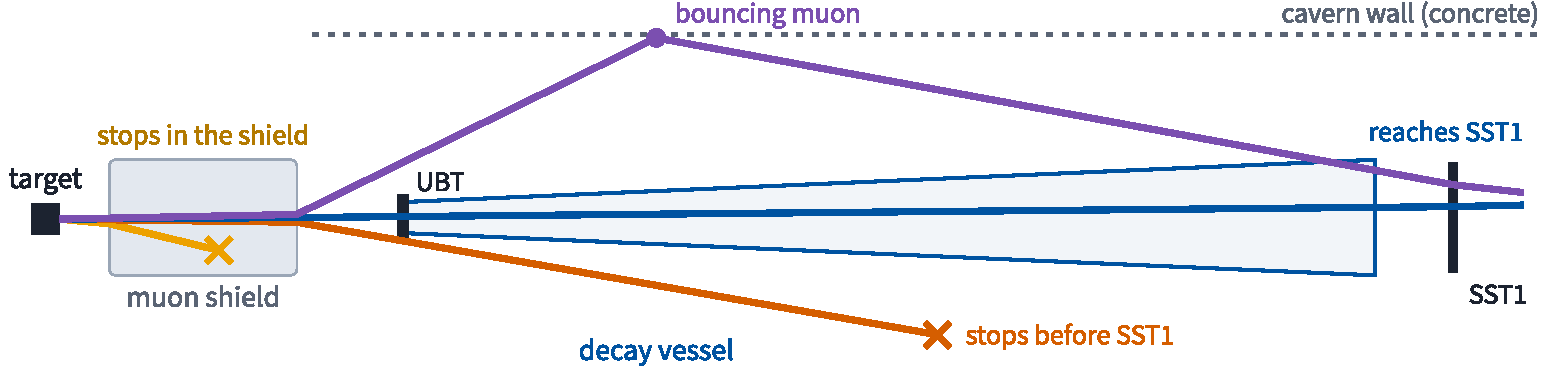
\includegraphics[width=1.00\linewidth,height=59.18pt,keepaspectratio]{figs/s38_sk1.pdf}\par}
\vspace{2.46pt}
\noindent \begin{minipage}[t]{\dimexpr(0.5000\linewidth-0.5000\dimexpr11.49pt\relax)}\vspace{0pt}\raggedright
{\fontsize{5.71pt}{7.42pt}\selectfont\setlength{\tabcolsep}{4.00pt}\renewcommand{\arraystretch}{1.42}
\begin{tabular}{lr}
\textcolor{muted}{Nov-4 muon category (type)} & \textcolor{muted}{per spill} \\\headrule
stop before z = 30.6 m (shield, TCC8 rock) & 4.38×10\textsuperscript{10} \\\rowrule
fly past the vessel / into the hall walls & 2.42×10\textsuperscript{9} \\\rowrule
stop between 30.6 and 82 m (cavern rock) & 6.75×10\textsuperscript{8} \\\rowrule
in the rock at 82 m & 1.48×10\textsuperscript{7} \\\rowrule
cross the vessel region, miss SST1 & 2.49×10\textsuperscript{4} \\\rowrule
\rowcolor{tint}\bfseries SST1, bounced off the cavern wall / floor & \bfseries 1.09×10\textsuperscript{4} \\\rowrule
\rowcolor{tint}\bfseries SST1, straight, good track (p > 1 GeV, 4 stations + TD) & \bfseries 6.05×10\textsuperscript{3} \\\rowrule
\rowcolor{tint}\bfseries SST1, other (soft or outside the stations / TD) & \bfseries 1.49×10\textsuperscript{4} \\\rowrule
\end{tabular}\par}
\end{minipage}%
\hfill%
\begin{minipage}[t]{\dimexpr(0.5000\linewidth-0.5000\dimexpr11.49pt\relax)}\vspace{0pt}\raggedright
{\fontsize{6.15pt}{8.60pt}\selectfont
\begin{itemize}
  \item Every muon is followed from the target to z = 30.6 m and to SST1; its type is set by where it ends
  \item \textbf{Bounced}: leave the vessel region, scatter in the cavern concrete and come back into SST1; their straight backward line misses the planes they crossed (bounce search)
  \item \textbf{Straight, p > 1 GeV, 4 straw stations + TD}: the good tracks of the pair candidates
\end{itemize}}
\end{minipage}\par
\end{btframe}

% ---------------------------------------------------------------- slide 39b: Nov-4 muon flux vs 2018 (19 Nov 2026)
\begin{btframe}{7 · Back-up · muon flux vs 2018}{Muon flux at the target: Nov-4 production vs the 2018 FairShip sample}
{\centering 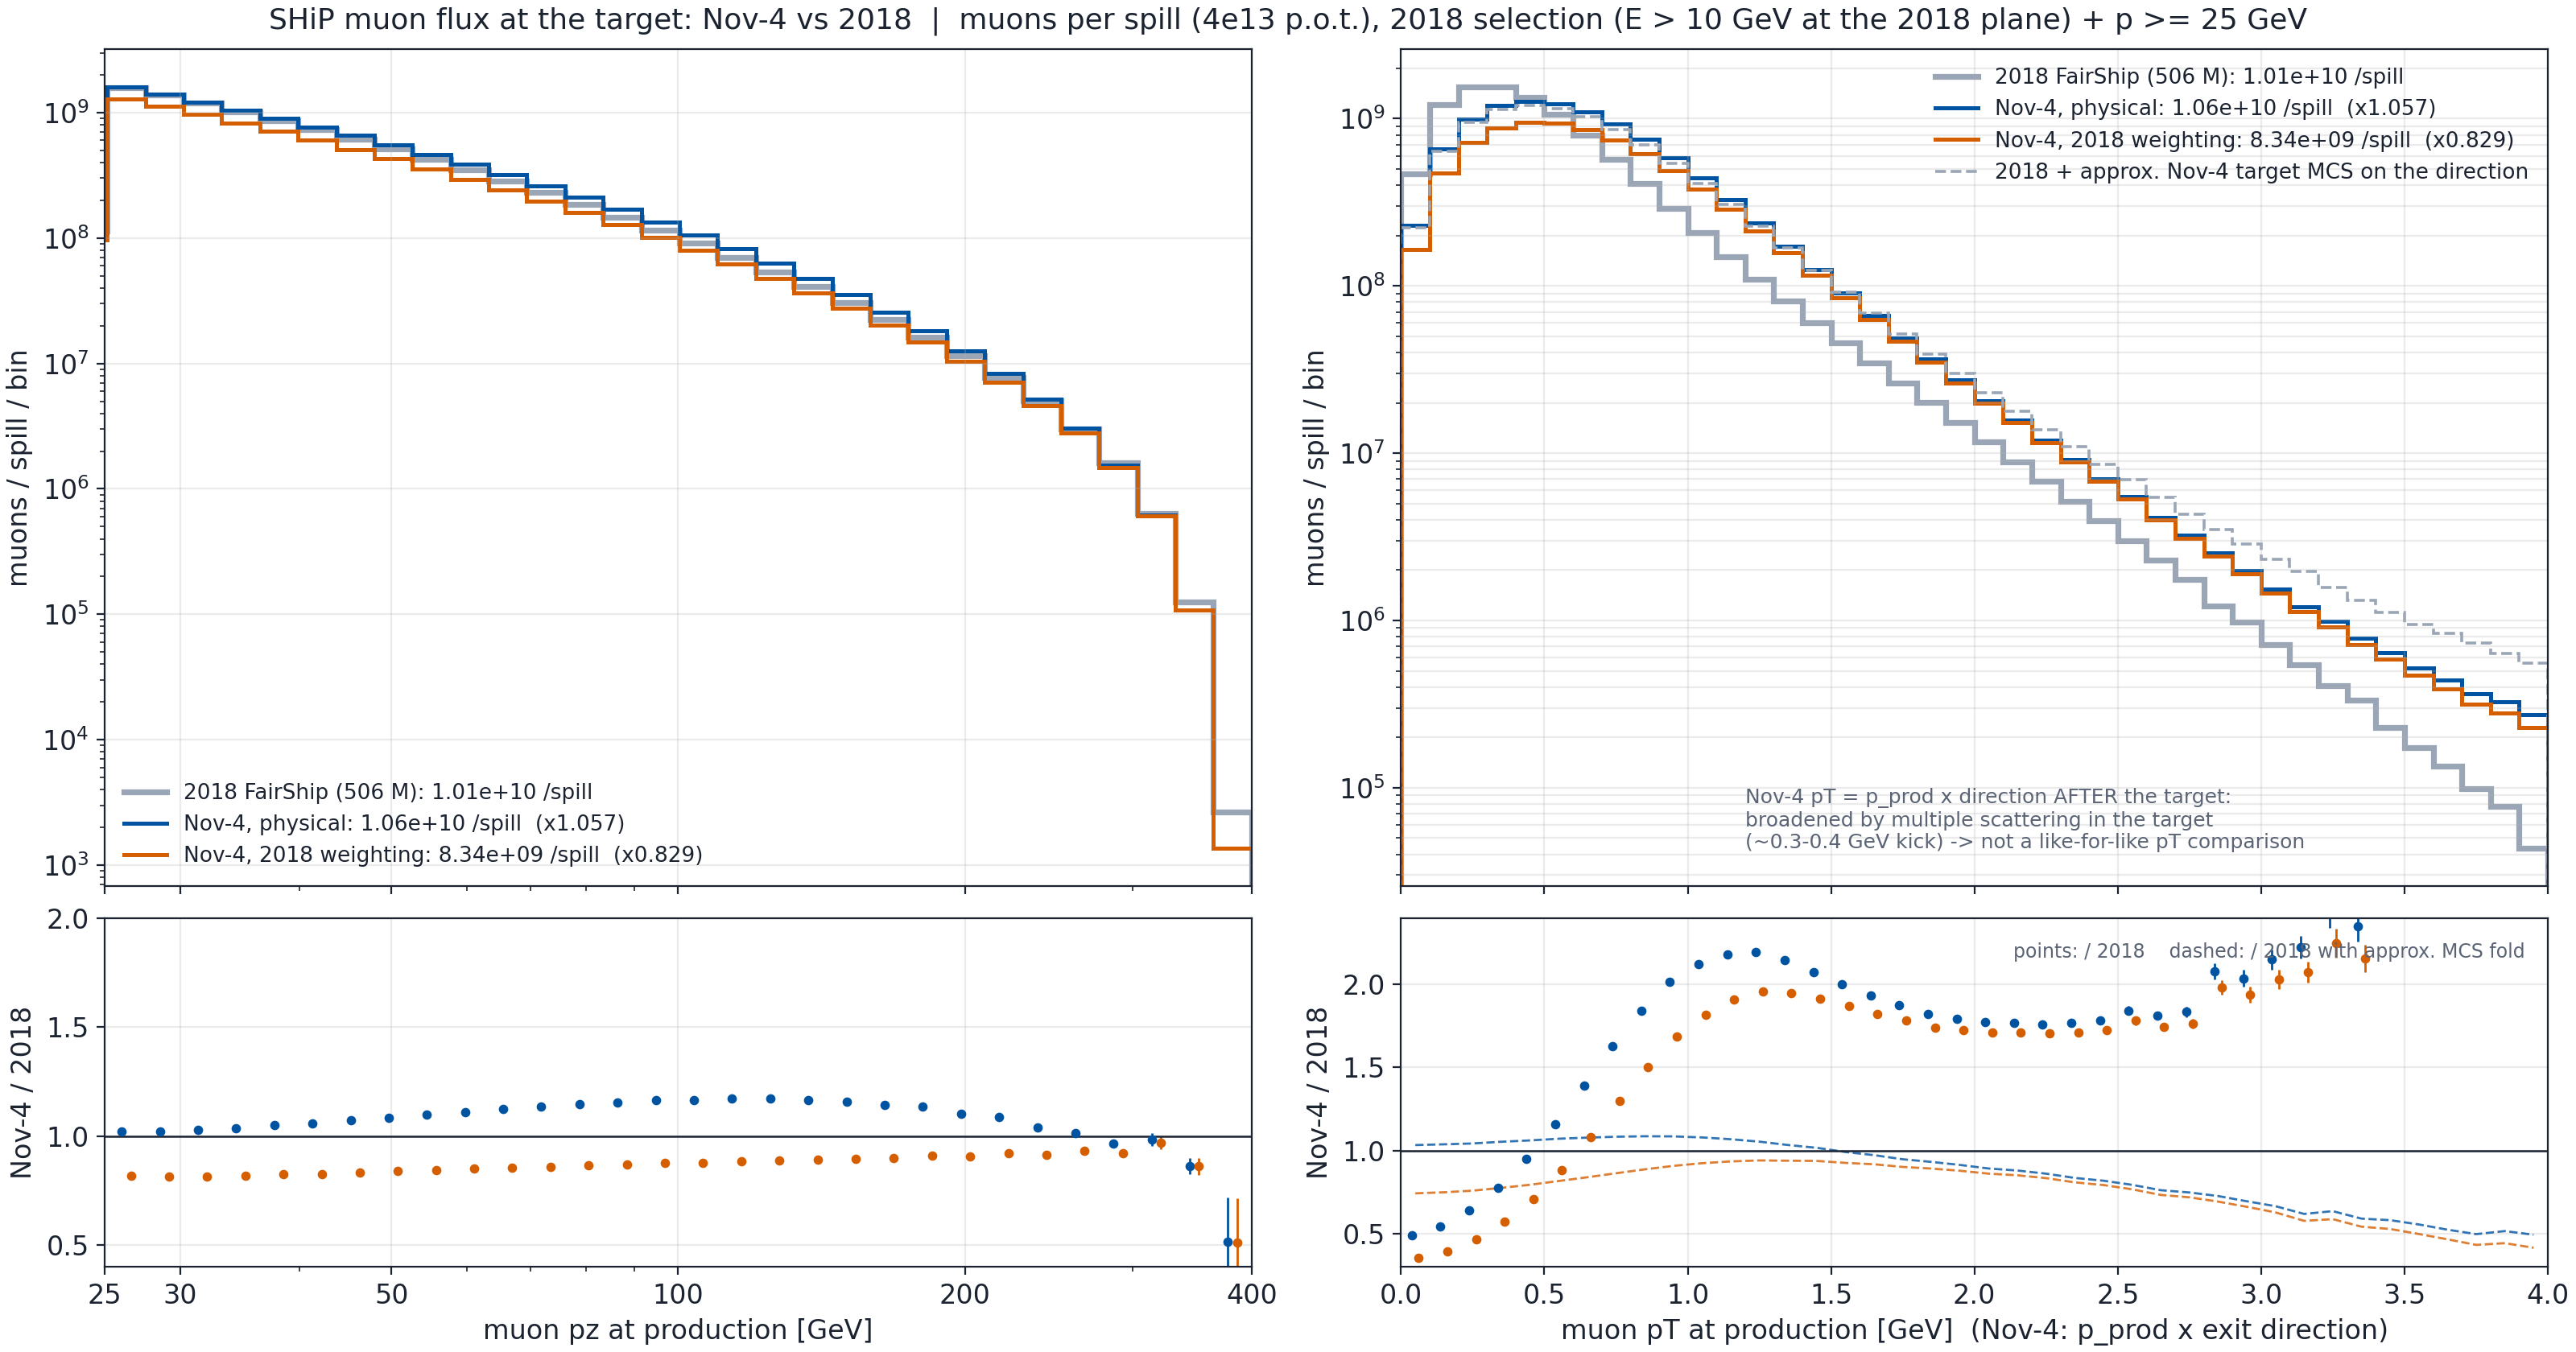
\includegraphics[height=138pt,keepaspectratio]{figs/s39b_nov4_vs_2018.png}\par}
\vspace{1.5pt}
{\fontsize{5.9pt}{8.0pt}\selectfont
\begin{itemize}
  \item Same 2018 selection on both (E > 10 GeV at the 2018 plane, p ≥ 25 GeV): Nov-4 / 2018 = \textbf{1.057}; charm, beauty, onia 0.98–1.00
  \item With FairShip's \textbf{2018 weighting emulated} (η → μμγ, ω → π\textsuperscript{0}μμ muons /100 without the ×100 boost): \textbf{0.83} → the 2018 files lack \textasciitilde{}22–27 \% of the min-bias flux
  \item p\textsubscript{T} is not like-for-like: Nov-4 keeps only the direction after the target (dashed: 2018 with approximate target scattering)
\end{itemize}}
\end{btframe}

% ---------------------------------------------------------------- 23 Nov 2026: how the cavern-rock x mu pairs form (4-station + TD good track, preliminary)
\begin{btframe}{7 · Back-up · cavern-rock × μ pairs}{Cavern-rock × μ pairs: where the vertex is and which particles (4 stations + TD, DOCA < 1 cm)}
\noindent \begin{minipage}[t]{\dimexpr(0.50\linewidth-0.50\dimexpr9.67pt\relax)}\vspace{0pt}\centering
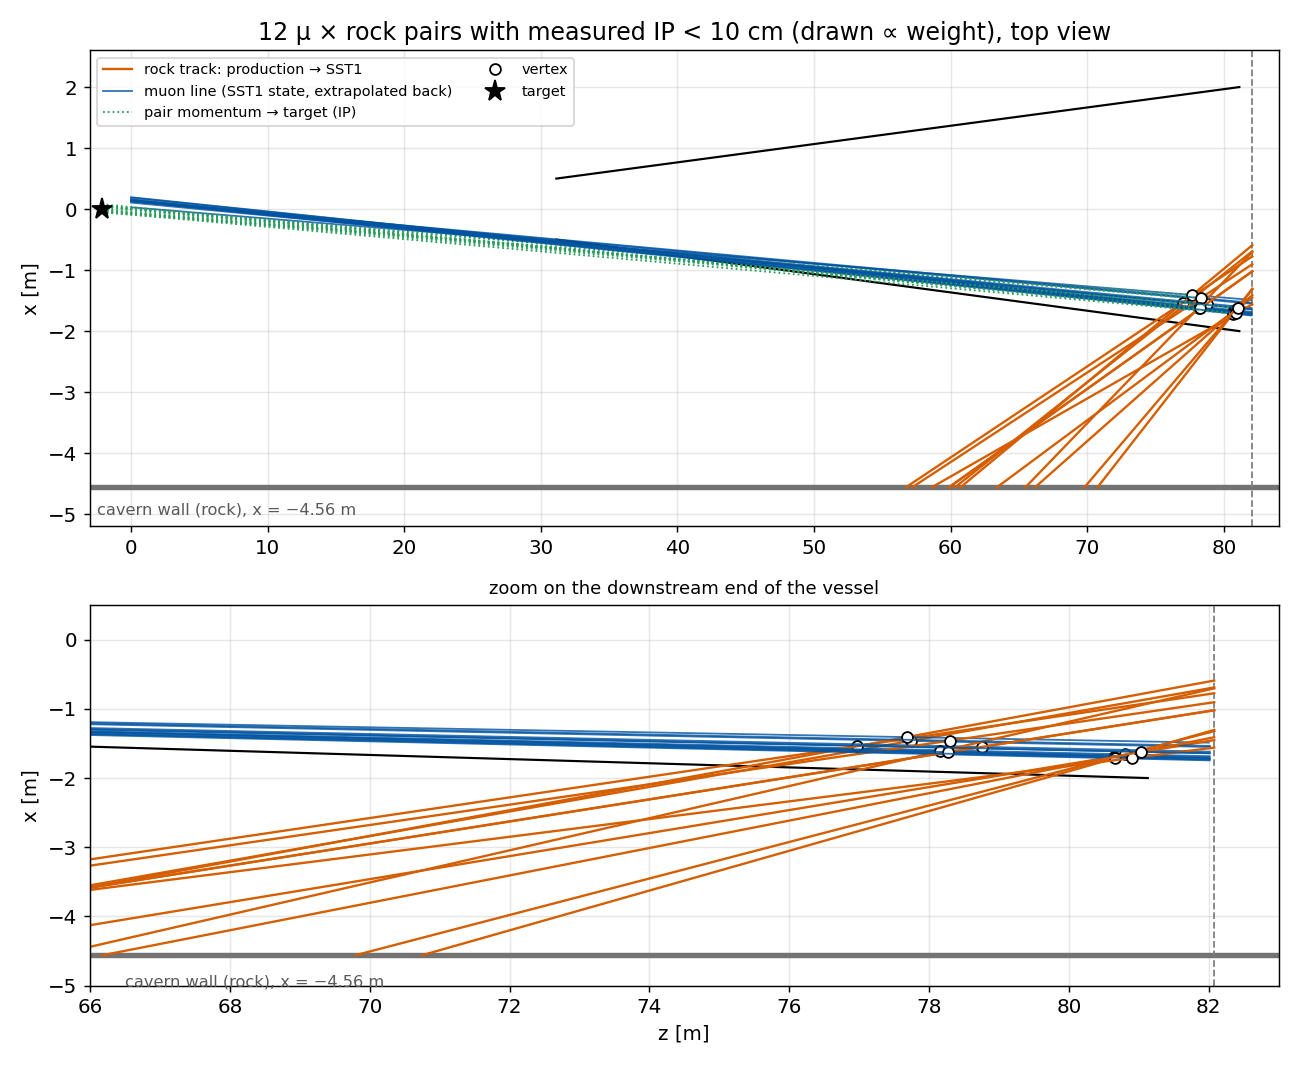
\includegraphics[width=\linewidth,height=165pt,keepaspectratio]{figs/s47_rock_mu_pairs_doca1.png}\par
\end{minipage}%
\hfill%
\begin{minipage}[t]{\dimexpr(0.50\linewidth-0.50\dimexpr9.67pt\relax)}\vspace{0pt}\raggedright
\begin{itemize}
  \item \textbf{Rock leg:} soft negative hadron (median 1.8 GeV) from the −x cavern wall at z ≈ 59–69 m, entering the vessel through the −x wall
  \item \textbf{Muon leg:} hard μ\textsuperscript{+} (median 222 GeV) along the −x wall; alone it misses the target by +18 cm
  \item \textbf{Vertex:} large opening angle (220 mrad) → closest approach just inside the −x wall, z ≈ 77–81 m; the rock leg tilts the pair onto the target (+3 cm)
\end{itemize}
\vspace{2pt}
{\fontsize{5.02pt}{6.52pt}\selectfont\setlength{\tabcolsep}{3.2pt}\renewcommand{\arraystretch}{1.42}
\begin{tabularx}{\linewidth}{>{\raggedright\arraybackslash}Xrrrr}
\textcolor{muted}{pairs / 15 y, before tagging (PDG μ, rock)} & \textcolor{muted}{w\textsubscript{μ} / spill} & \textcolor{muted}{w\textsubscript{rock} / spill} & \textcolor{muted}{IP < 10 cm} & \textcolor{muted}{share} \\\headrule
μ\textsuperscript{+} × π\textsuperscript{−} (−13, −211) & 0.0025 & 4.6 & 30.9 & 73 \% \\\rowrule
μ\textsuperscript{+} × K\textsuperscript{−} (−13, −321) & 0.0025 & 4.5 & 5.7 & 14 \% \\\rowrule
μ\textsuperscript{+} × p̄ (−13, −2212) & 0.0025 & 4.4 & 3.2 & 8 \% \\\rowrule
μ\textsuperscript{+} × e\textsuperscript{−} (−13, 11) & 0.0025 & 4.9 & 2.0 & 5 \% \\\rowrule
μ\textsuperscript{−} × positive (13, +) & & & 0.05 & 0 \\\rowrule
\rowcolor{tint}\bfseries total (candidates 110, IP < 2.5 m 108) & & & \bfseries 42 & \\\rowrule
\end{tabularx}\par}
\vspace{2pt}
\begin{itemize}
  \item 4 stations + TD on both legs, DOCA < 1 cm, all muons: 110 / 42 / 108 per 15 y (DOCA < 2 cm: 220 / 84 / 216; old SST1 + TD: 634 / 211 / 626); weights = median per leg
  \item After tagging: R1 0.097 ± 0.012, R2 < 0.027 (90 \% CL), Z1 1.2×10\textsuperscript{-5}
\end{itemize}
\end{minipage}\par
\end{btframe}

% ---------------------------------------------------------------- 24 Nov 2026: cavern-rock x mu vertices with the pair lines, and vertex z (4-station + TD, preliminary)
\begin{btframe}{7 · Back-up · cavern-rock × μ vertices}{Cavern-rock × μ vertices in the vessel (4 stations + TD, DOCA < 1 cm)}
\centering
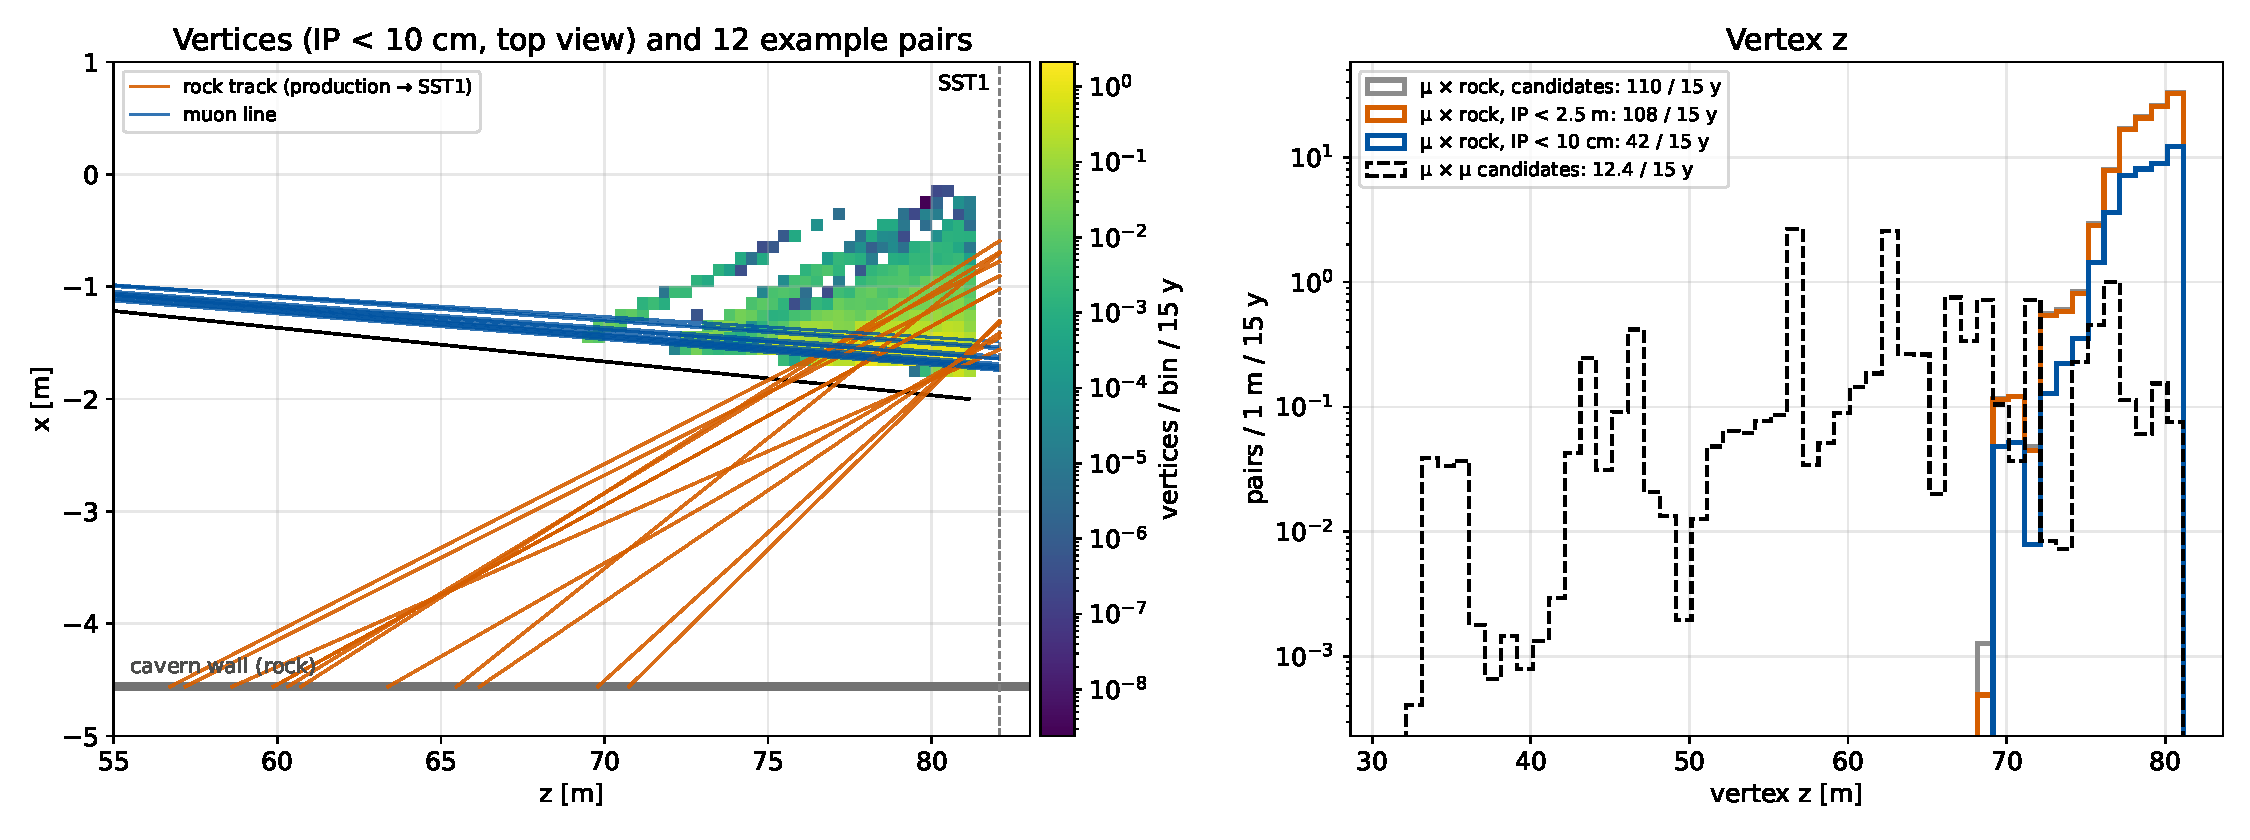
\includegraphics[width=0.96\linewidth,height=170pt,keepaspectratio]{figs/s48_rock_mu_vertices_doca1.pdf}\par
\vspace{4pt}
\raggedright
\begin{itemize}\footnotesize
  \item Left: vertices of the pairs with measured IP < 10 cm (top view, per 15 y) and 12 example pairs: rock tracks (orange) from the −x cavern wall cross the muon lines (blue) just inside the −x vessel wall
  \item Right: vertex z at each cut, μ × μ for comparison: all μ × rock vertices in the last ~10 m of the vessel (median 79.1 m), μ × μ spread over the whole vessel
\end{itemize}
\end{btframe}
% ---------------------------------------------------------------- back-up: x-z maps of the combinatorial pair vertices (24 Nov 2026)
\begin{btframe}{7 · Back-up · combinatorial vertices}{Where the combinatorial vertices are: MS7 interaction × μ and cavern rock × μ (DOCA < 1 cm)}
\centering
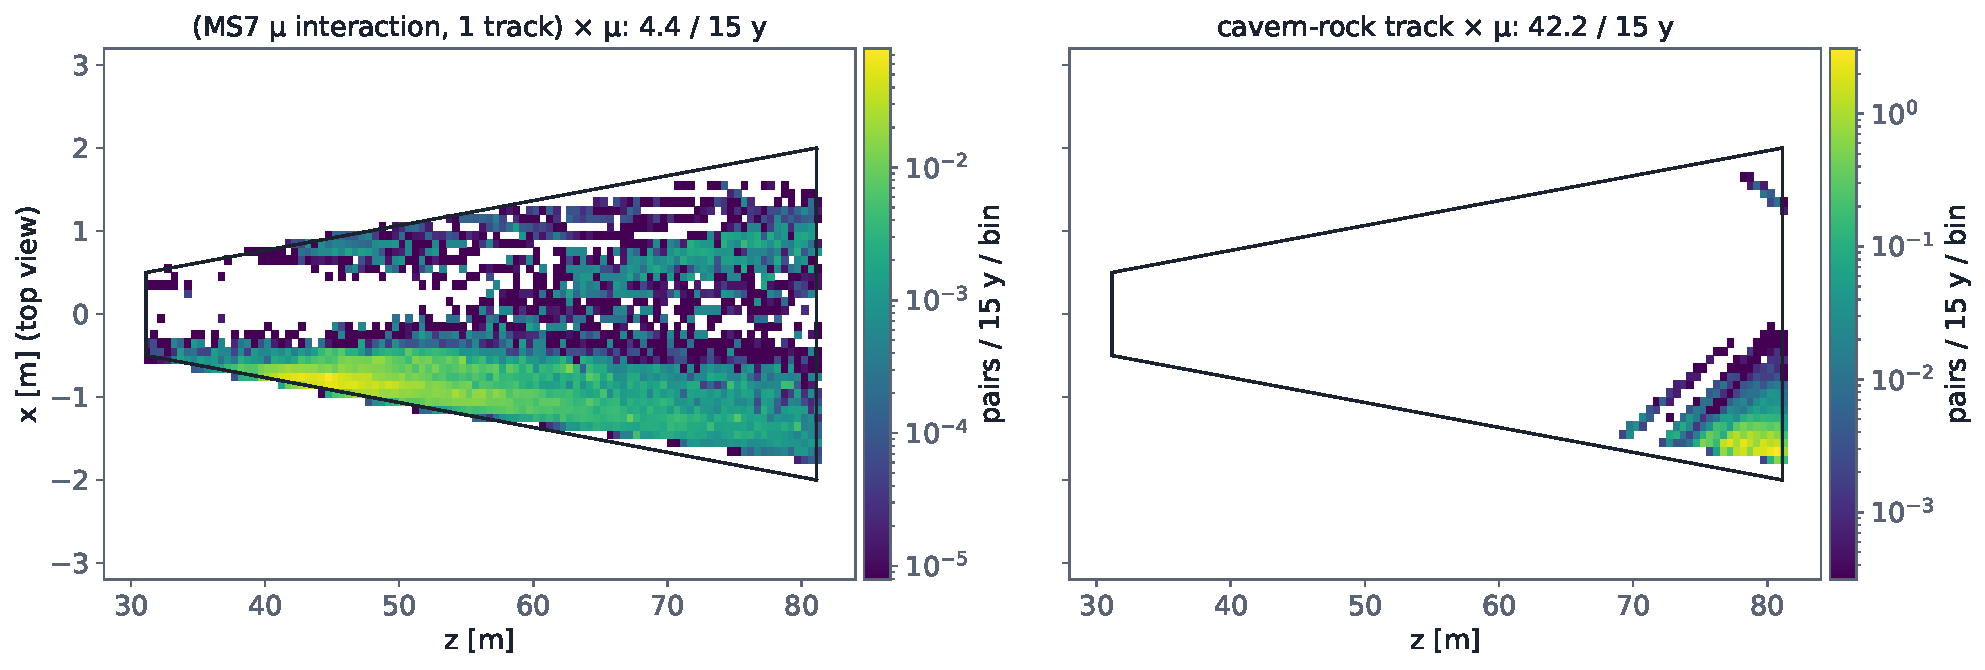
\includegraphics[width=\linewidth,height=150pt,keepaspectratio]{figs/s20_pairs_xz_doca1.pdf}\par
\vspace{4pt}
\raggedright
\begin{itemize}\footnotesize
  \item Top view of the pair vertices with measured IP < 10 cm, per 15 y, 4-station good track; vessel outline in black
  \item MS7 interaction (1 track) × μ: 4.4 / 15 y, spread over the whole vessel near the −x wall; cavern rock × μ: 42 / 15 y, last ~10 m, −x side
\end{itemize}
\end{btframe}

% ---------------------------------------------------------------- slide 40: MS7 KL: from production to SST1, and the comparison with data
\begin{btframe}{7 · Back-up · MS7 K\textsubscript{L}}{MS7 K\textsubscript{L}: from production to SST1, and the comparison with data}
\noindent \begin{minipage}[t]{\dimexpr(0.5556\linewidth-0.5556\dimexpr9.67pt\relax)}\vspace{0pt}\raggedright
{\fontsize{5.02pt}{6.52pt}\selectfont\setlength{\tabcolsep}{3.51pt}\renewcommand{\arraystretch}{1.42}
\begin{tabularx}{\linewidth}{>{\raggedright\arraybackslash}Xrr}
\textcolor{muted}{step} & \textcolor{muted}{per spill} & \textcolor{muted}{note} \\\headrule
muons crossing the last 50 cm of MS7 & 4.6×10\textsuperscript{8} & Nov-4 transport \\\rowrule
muon interactions (Geant4 muonNuclear) & 8.0×10\textsuperscript{5} & P ≈ 1.7×10\textsuperscript{-3} per muon \\\rowrule
K\textsubscript{L} made (vertex 7.8×10\textsuperscript{3} + shower 7.6×10\textsuperscript{3}) & 1.5×10\textsuperscript{4} & 0.0099 per interaction at the vertex \\\rowrule
K\textsubscript{L} leaving the iron (T > 0.5 GeV) & 3.2×10\textsuperscript{3} & absorption λ ≈ 19 cm \\\rowrule
K\textsubscript{L} decaying in the vessel & 1.5×10\textsuperscript{3} – 2.0×10\textsuperscript{3} & 49 \% of those leaving \\\rowrule
\rowcolor{tint}\bfseries two good tracks, pair cuts (DOCA < 1 cm) & \bfseries 0.78 & \bfseries 1.17×10\textsuperscript{7} / 15 y \\\rowrule
\rowcolor{tint}\bfseries IP < 10 cm (full selection) & \bfseries 8.1×10\textsuperscript{-4} & \bfseries 1.22×10\textsuperscript{4} / 15 y \\\rowrule
\end{tabularx}\par}
\end{minipage}%
\hfill%
\begin{minipage}[t]{\dimexpr(0.4444\linewidth-0.4444\dimexpr9.67pt\relax)}\vspace{0pt}\raggedright
{\fontsize{5.02pt}{6.52pt}\selectfont\setlength{\tabcolsep}{3.51pt}\renewcommand{\arraystretch}{1.42}
\begin{tabularx}{\linewidth}{>{\raggedright\arraybackslash}Xrrr}
\textcolor{muted}{V0 per event, W = 6.2 GeV} & \textcolor{muted}{K\textsubscript{S}} & \textcolor{muted}{Λ (+Σ\textsuperscript{0})} & \textcolor{muted}{Λ̄} \\\headrule
γp, E\textsubscript{γ} = 20 GeV (SLAC) & 0.082 ± 0.003 & 0.049 ± 0.002 & 0.0029 ± 0.0003 \\\rowrule
\rowcolor{tint}\bfseries Geant4 11.2 muonNuclear & \bfseries 0.087 & \bfseries 0.051 & \bfseries 0.0020 \\\rowrule
Pythia 6 & 0.153 & 0.090 & 0.0058 \\\rowrule
\end{tabularx}\par}
\vspace{2.46pt}
{\fontsize{4.78pt}{6.45pt}\selectfont Geant4 reproduces the measured K\textsubscript{S} and Λ yields within 6 \% at W = 6.2 GeV; Pythia 6 is ×1.9 high. Most MS7 K\textsubscript{L} come from W = 5–10 GeV; low W (1.6–3 GeV) is not yet compared (ISSUES D16).\par}
\end{minipage}\par
\end{btframe}

% ---------------------------------------------------------------- slide 40q: Q2 and W of the interactions that make the MS7 KL (19 Nov 2026)
\begin{btframe}{7 · Back-up · MS7 K\textsubscript{L} production}{Which muon interactions make the MS7 K\textsubscript{L}: Q\textsuperscript{2} and W}
\begin{minipage}[t]{0.27\linewidth}\vspace{0pt}\centering
{\fontsize{5.5pt}{6.5pt}\selectfont Geant4 11.2 muonNuclear (default)\par}
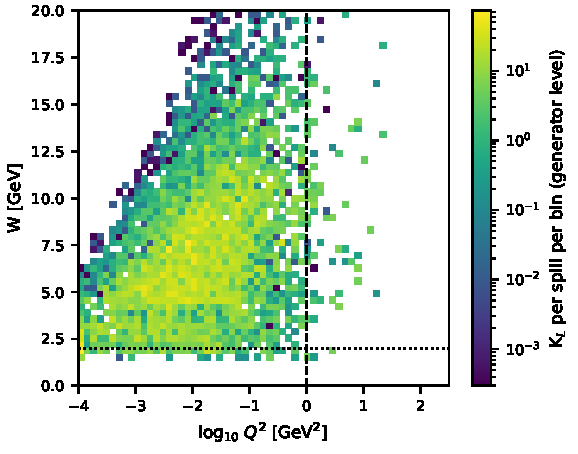
\includegraphics[width=\linewidth]{figs/kl_q2w_geant4.pdf}
\end{minipage}\hfill
\begin{minipage}[t]{0.27\linewidth}\vspace{0pt}\centering
{\fontsize{5.5pt}{6.5pt}\selectfont Pythia 6\par}
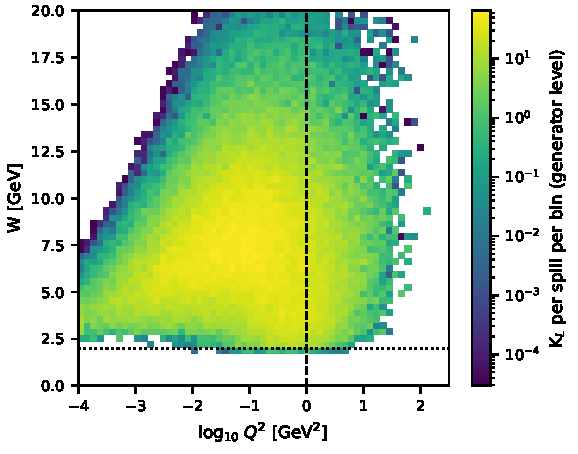
\includegraphics[width=\linewidth]{figs/kl_q2w_pythia6.pdf}
\end{minipage}\hfill
\begin{minipage}[t]{0.42\linewidth}\vspace{0pt}
{\fontsize{5.9pt}{7.9pt}\selectfont
\begin{itemize}
  \item Geant4: 96 \% of the interactions have Q\textsuperscript{2} < 0.1 GeV\textsuperscript{2} and 72 \% W < 2 GeV, but they make almost no K\textsubscript{L}
  \item \textcolor{cern}{\textbf{The K\textsubscript{L} come from W = 5–10 GeV (55 \%) and W > 10 GeV (15 \%)}}: 5 \% of the interactions, still at Q\textsuperscript{2} < 1 GeV\textsuperscript{2} (98 \%)
  \item Pythia 6 fills the same region but makes ≈ 14× more K\textsubscript{L} per interaction there
  \item \textbf{Quasi-real photoproduction at W ≈ 3–10 GeV}, where γp data exist: used to choose the generator (next slides)
\end{itemize}}
\end{minipage}
\vspace{2pt}
{\centering 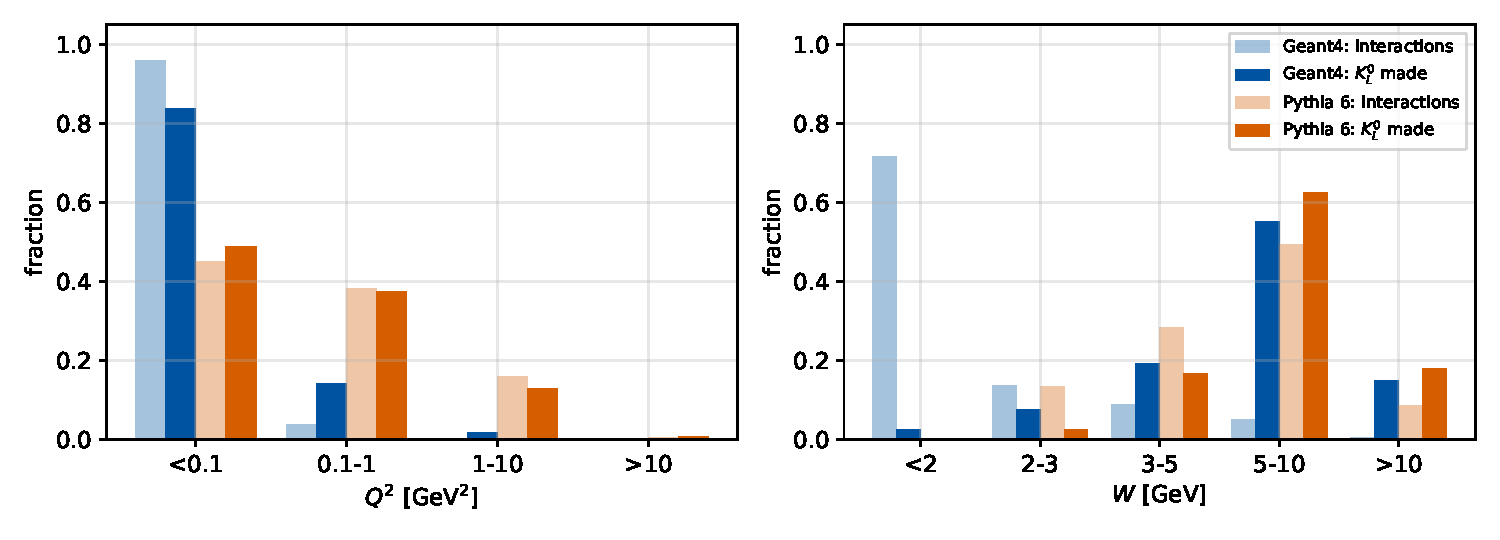
\includegraphics[width=0.80\linewidth,height=88pt,keepaspectratio]{figs/int_kl_q2w_shares.pdf}\par}
\begin{tikzpicture}[remember picture,overlay]
\node[anchor=north east,inner sep=0] (t1) at ([xshift=-14pt,yshift=-6pt]current page.north east) {
\includegraphics[width=125pt]{figs/talk_2.png}};
\end{tikzpicture}
\end{btframe}

% ---------------------------------------------------------------- slide 40a1: MS7 KL production, Geant4 vs Pythia vs data (19 Nov 2026)
\begin{btframe}{7 · Back-up · MS7 K\textsubscript{L} production}{MS7 K\textsubscript{L}: what we know, Geant4 and Pythia against the data}
{\centering 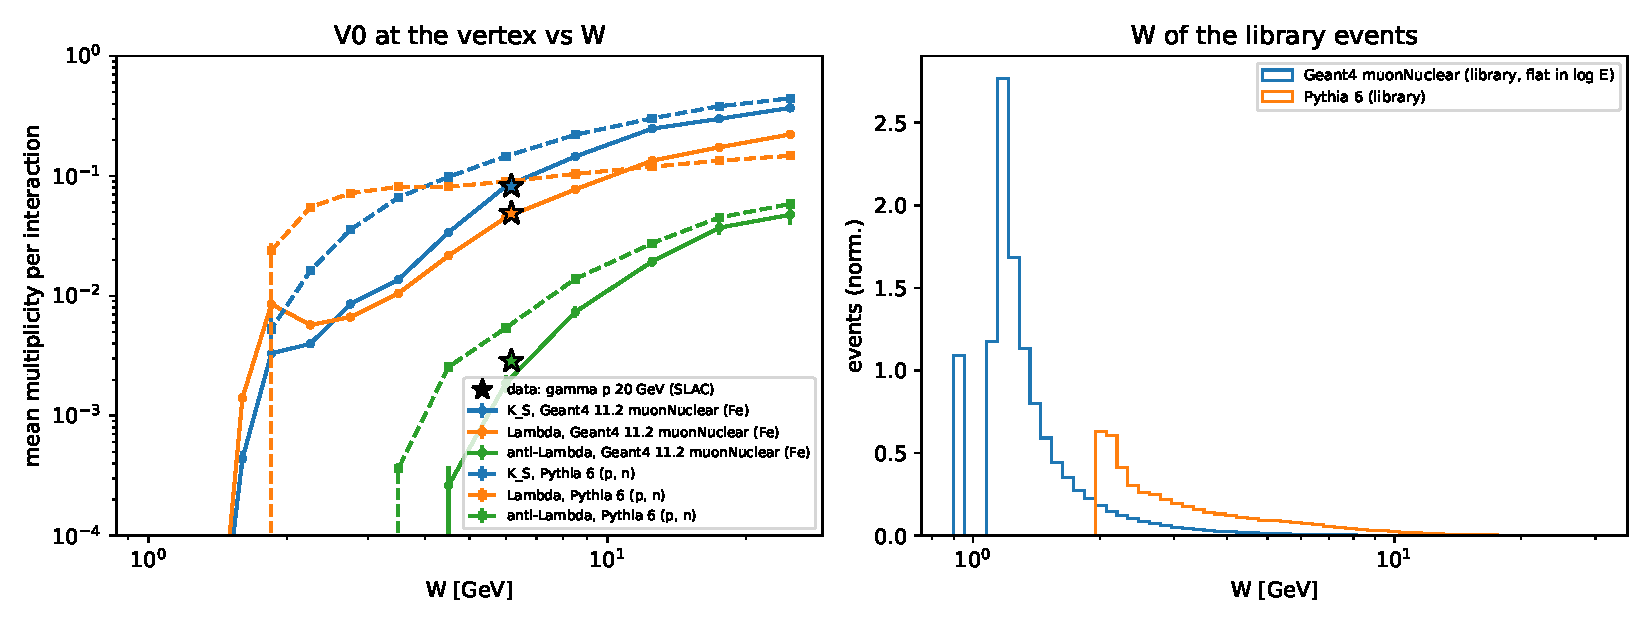
\includegraphics[width=0.86\linewidth,height=118pt,keepaspectratio]{figs/v0_vs_W.pdf}\par}
\vspace{2.46pt}
{\fontsize{5.9pt}{7.9pt}\selectfont
\begin{itemize}
  \item \textbf{Generators:} \textcolor{cern}{\textbf{Geant4 11.2 muonNuclear}} on Fe (default; median W 1.3 GeV, mostly below the K Λ threshold) and \textbf{Pythia 6.4.28} γ\textsuperscript{*} on p, n (W > 2 GeV only). Per interaction: K\textsubscript{L} 0.0099 (Geant4) vs 0.12 (Pythia), mostly from their different W spectra (right)
  \item \textbf{K\textsubscript{L} is not measured directly:} K\textsuperscript{0}, \=K\textsuperscript{0} give ½ K\textsubscript{S} + ½ K\textsubscript{L}, so K\textsubscript{L} = K\textsubscript{S} and the K\textsubscript{S} data validate it
  \item \textbf{Data:} SLAC γp at E\textsubscript{γ} = 20 GeV (W = 6.2 GeV, stars): K\textsubscript{S} 0.082 ± 0.003, Λ 0.049 ± 0.002 per event. \textcolor{cern}{\textbf{Geant4 within 6 \%}}, Pythia ×1.9 high. Cross-check: NOMAD ν\textsubscript{μ} CC on C, K\textsubscript{S} 0.068 per event
  \item \textbf{Chain (per spill):} 1.5×10\textsuperscript{4} K\textsubscript{L} made (half by the shower in the iron) → 3.2×10\textsuperscript{3} leave the iron (37 \% from the shower) → 1.5×10\textsuperscript{3} decay in the vessel. Geant4 11.4 and 11.2 agree within 1–3 \%
\end{itemize}}
\slidenote{Data: K. Abe et al., PRD 30 (1984) 1 (SLAC SHF, Table II); NOMAD: P. Astier et al., NPB 621 (2002) 3.}
\end{btframe}

% ---------------------------------------------------------------- slide 40a2: MS7 KL production at low W (19 Nov 2026)
\begin{btframe}{7 · Back-up · MS7 K\textsubscript{L} production}{Strangeness at low W: where most Geant4 interactions are}
{\centering 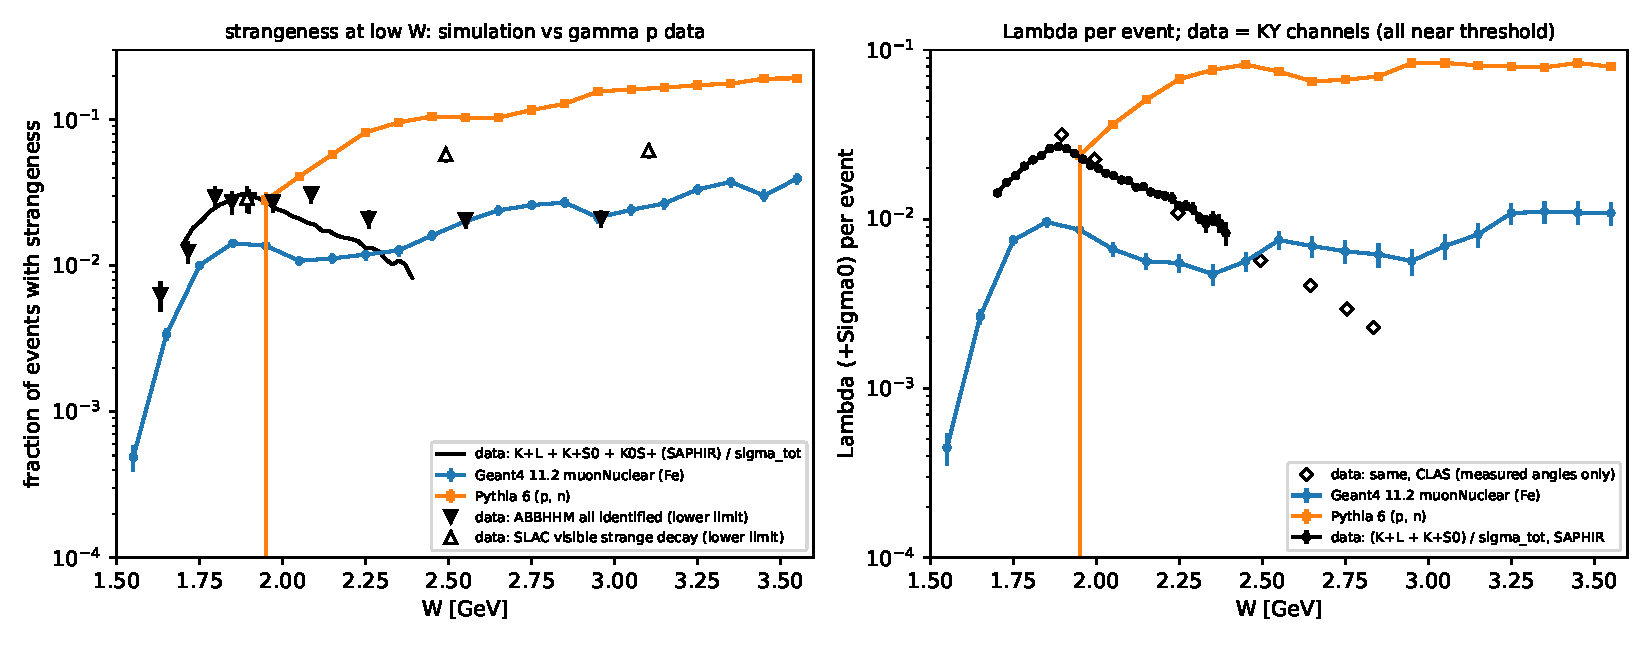
\includegraphics[width=0.86\linewidth,height=118pt,keepaspectratio]{figs/v0_lowW.pdf}\par}
\vspace{2.46pt}
{\fontsize{5.9pt}{7.9pt}\selectfont
\begin{itemize}
  \item \textbf{Data (γp, near threshold, all lower limits):} SAPHIR and CLAS exclusive K Λ, K Σ cross sections over σ\textsubscript{tot}; ABBHHM identified strange final states; SLAC visible strange decays
  \item Geant4 is \textbf{low by ≥ ×2} for W < 2.2 GeV and by ≥ ×2.5–3 at W = 2.5–3 GeV; Pythia (W > 2 GeV) is ×3–5 above the exclusive Λ channels
  \item \textbf{Impact is small:} of the vertex K\textsubscript{L} that can leave the iron (T > 0.5 GeV), \textcolor{cern}{\textbf{78 \% come from W > 5 GeV}} (validated, previous slide), 14 \% from 3.5–5 GeV, 7.6 \% from W < 3.5 GeV. A ×2–3 deficit there gives \textbf{+8–15 \%} on the K\textsubscript{L}
  \item \textbf{Open:} W = 3.5–5 GeV not compared with data (14 \% of the relevant K\textsubscript{L}); the selected K\textsubscript{L} rest on 74 simulated events
\end{itemize}}
\slidenote{Data: SAPHIR (Glander 2004, Lawall 2005), CLAS (McCracken 2010, Dey 2010; measured angles only), ABBHHM (Erbe 1969), SLAC (Ballam 1969, Bingham 1973); σ\textsubscript{tot}: Armstrong 1972, Caldwell 1973.}
\end{btframe}

% ---------------------------------------------------------------- slide 40b: MS7 KL momentum, decay point and SST1 (19 Nov 2026)
\begin{btframe}{7 · Back-up · MS7 K\textsubscript{L} momentum}{MS7 K\textsubscript{L}: momentum at the decay point and of its charged products at SST1}
\begin{minipage}[t]{0.49\linewidth}\vspace{0pt}\centering
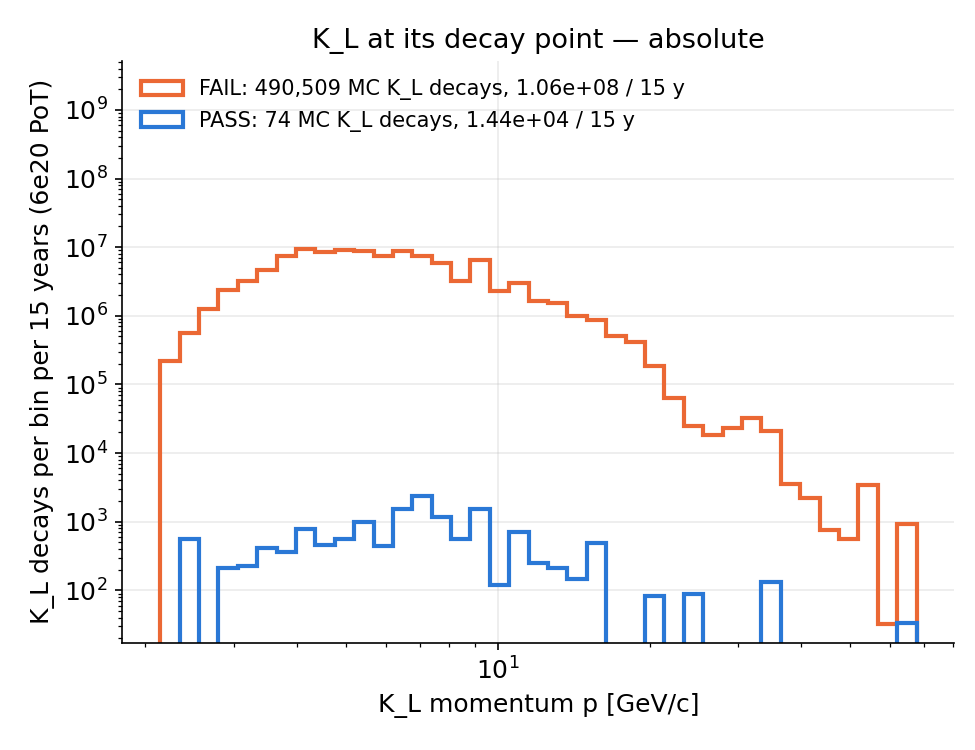
\includegraphics[width=0.84\linewidth]{figs/s40b_kl_p.png}
\end{minipage}\hfill
\begin{minipage}[t]{0.49\linewidth}\vspace{0pt}\centering
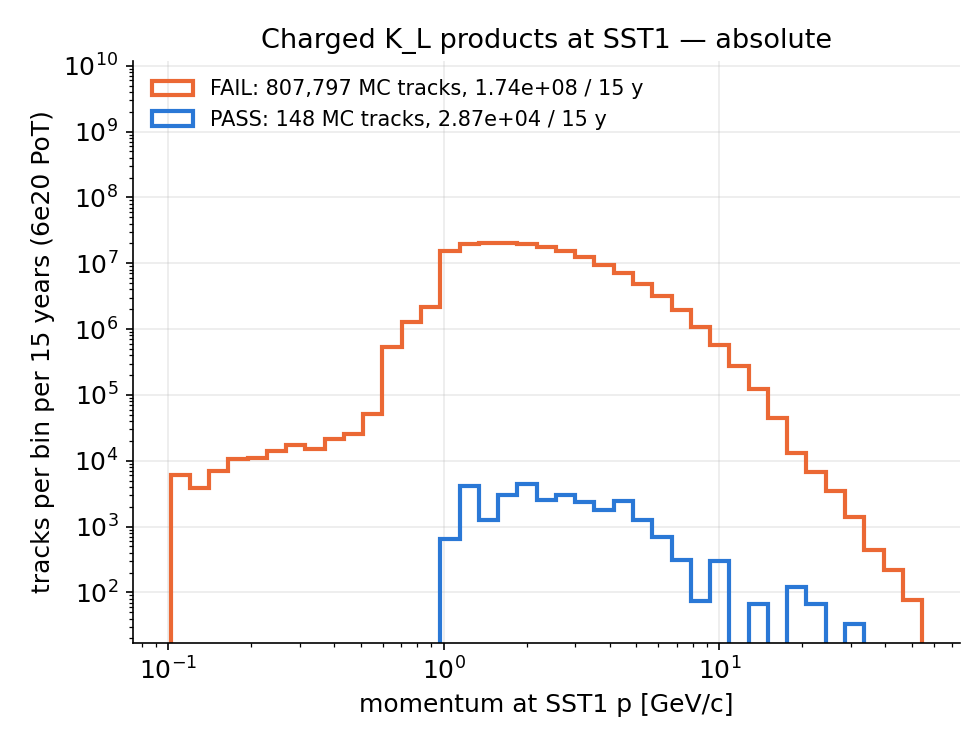
\includegraphics[width=0.84\linewidth]{figs/s40b_sst1_p.png}
\end{minipage}
\vspace{2.46pt}
{\fontsize{6.15pt}{8.60pt}\selectfont
\begin{itemize}
  \item \textcolor{cern}{\textbf{PASS}} the full selection: 74 simulated decays, 1.44×10\textsuperscript{4} / 15 y; \textbf{FAIL}: 4.9×10\textsuperscript{5} decays, 1.06×10\textsuperscript{8} / 15 y
  \item Selected K\textsubscript{L} are slightly harder (median 6.8 vs 5.6 GeV: \textbf{β = 0.9974} vs 0.9960, 0.36 ns behind light over 40 m) and decay further downstream (median z 72 vs 65 m)
  \item At SST1 the selected events have exactly two charged tracks, median 2.3 GeV (2.0 GeV for FAIL); none below the 1 GeV cut
\end{itemize}}
\end{btframe}

% ---------------------------------------------------------------- slide 40c: MS7 KL species, decay point and SST1 (19 Nov 2026)
\begin{btframe}{7 · Back-up · MS7 K\textsubscript{L} species}{MS7 K\textsubscript{L}: particles at the decay point and at SST1}
\begin{minipage}[t]{0.49\linewidth}\vspace{0pt}\centering
{\fontsize{5.5pt}{7pt}\selectfont\textcolor{muted}{at the decay point}\par}
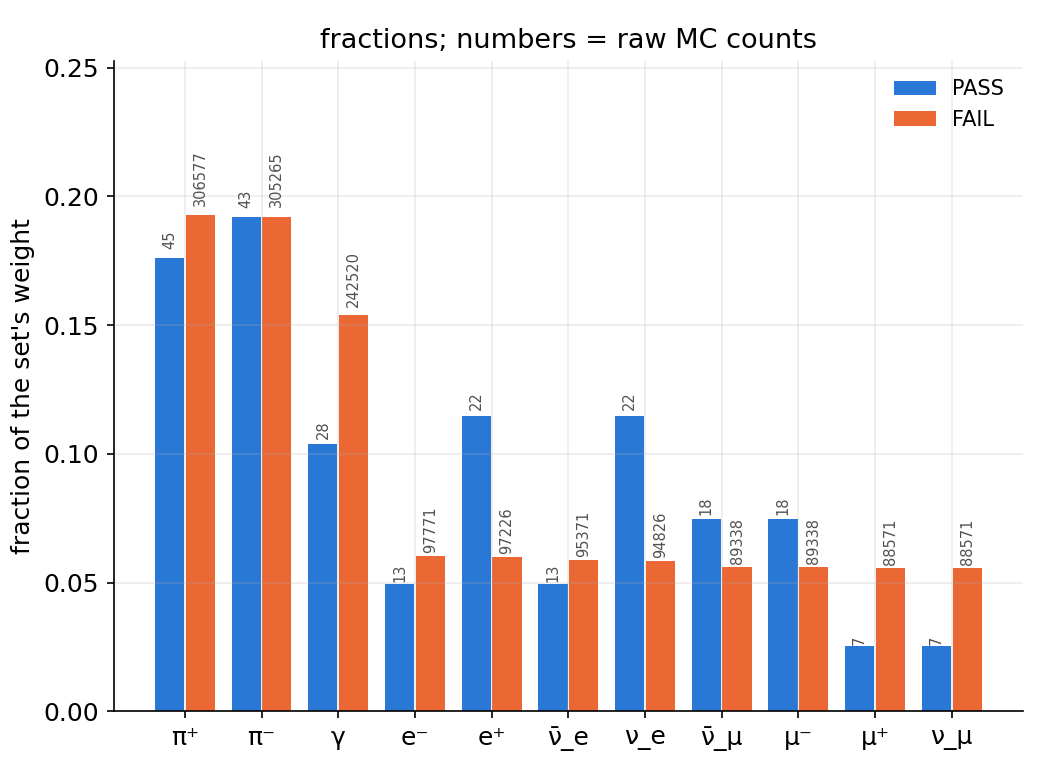
\includegraphics[width=0.92\linewidth]{figs/s40c_pdg_decay.png}
\end{minipage}\hfill
\begin{minipage}[t]{0.49\linewidth}\vspace{0pt}\centering
{\fontsize{5.5pt}{7pt}\selectfont\textcolor{muted}{K\textsubscript{L} products reaching SST1}\par}
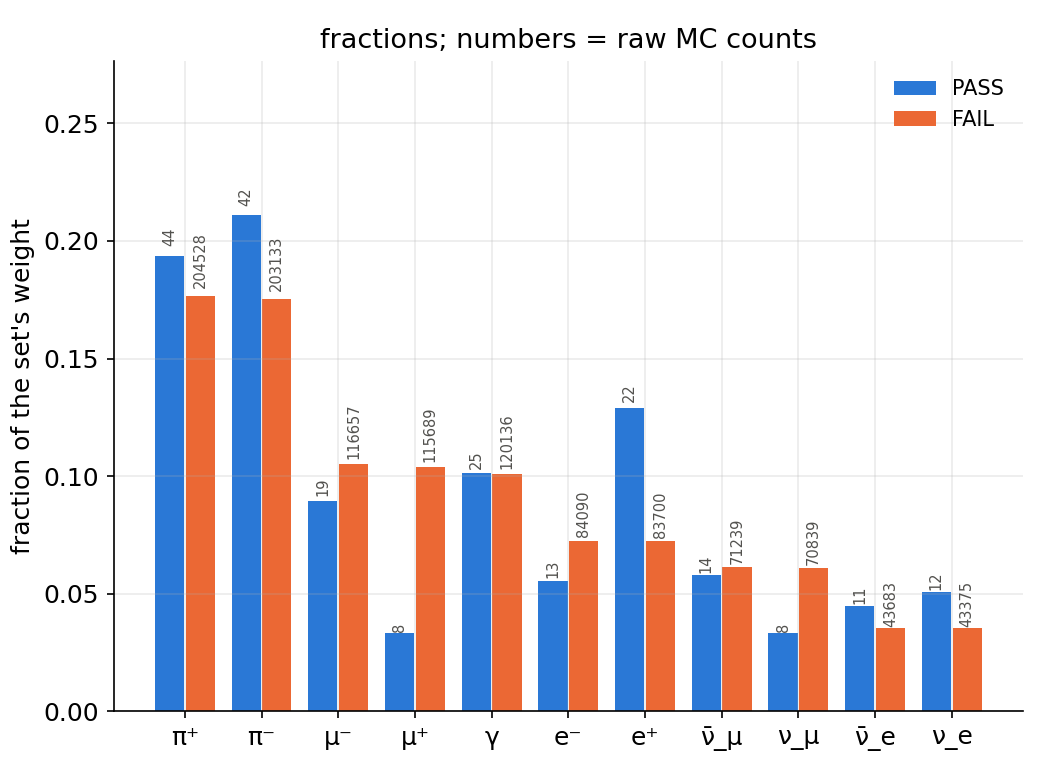
\includegraphics[width=0.92\linewidth]{figs/s40c_pdg_sst1.png}
\end{minipage}
\vspace{2.46pt}
{\fontsize{6.15pt}{8.60pt}\selectfont
\begin{itemize}
  \item Selected decays are mostly semileptonic: K\textsubscript{e3} 52 \%, K\textsubscript{μ3} 32 \%, π\textsuperscript{+}π\textsuperscript{−}π\textsuperscript{0} 16 \% (FAIL follows the decay table: π\textsuperscript{+}π\textsuperscript{−}π\textsuperscript{0} 25 \%)
  \item At SST1 the pions dominate both sets (\textasciitilde{}20 \% each charge); the e\textsuperscript{+} excess and μ\textsuperscript{+} deficit of PASS are within its statistics (74 events)
\end{itemize}}
\end{btframe}


% ---------------------------------------------------------------- slide 40d: Q2 and W of the parent interaction, PASS vs FAIL (20 Nov 2026)
\begin{btframe}{7 · Back-up · MS7 K\textsubscript{L} parent DIS}{MS7 K\textsubscript{L}: Q\textsuperscript{2} and W of the muon interaction that made it, PASS vs FAIL}
{\centering 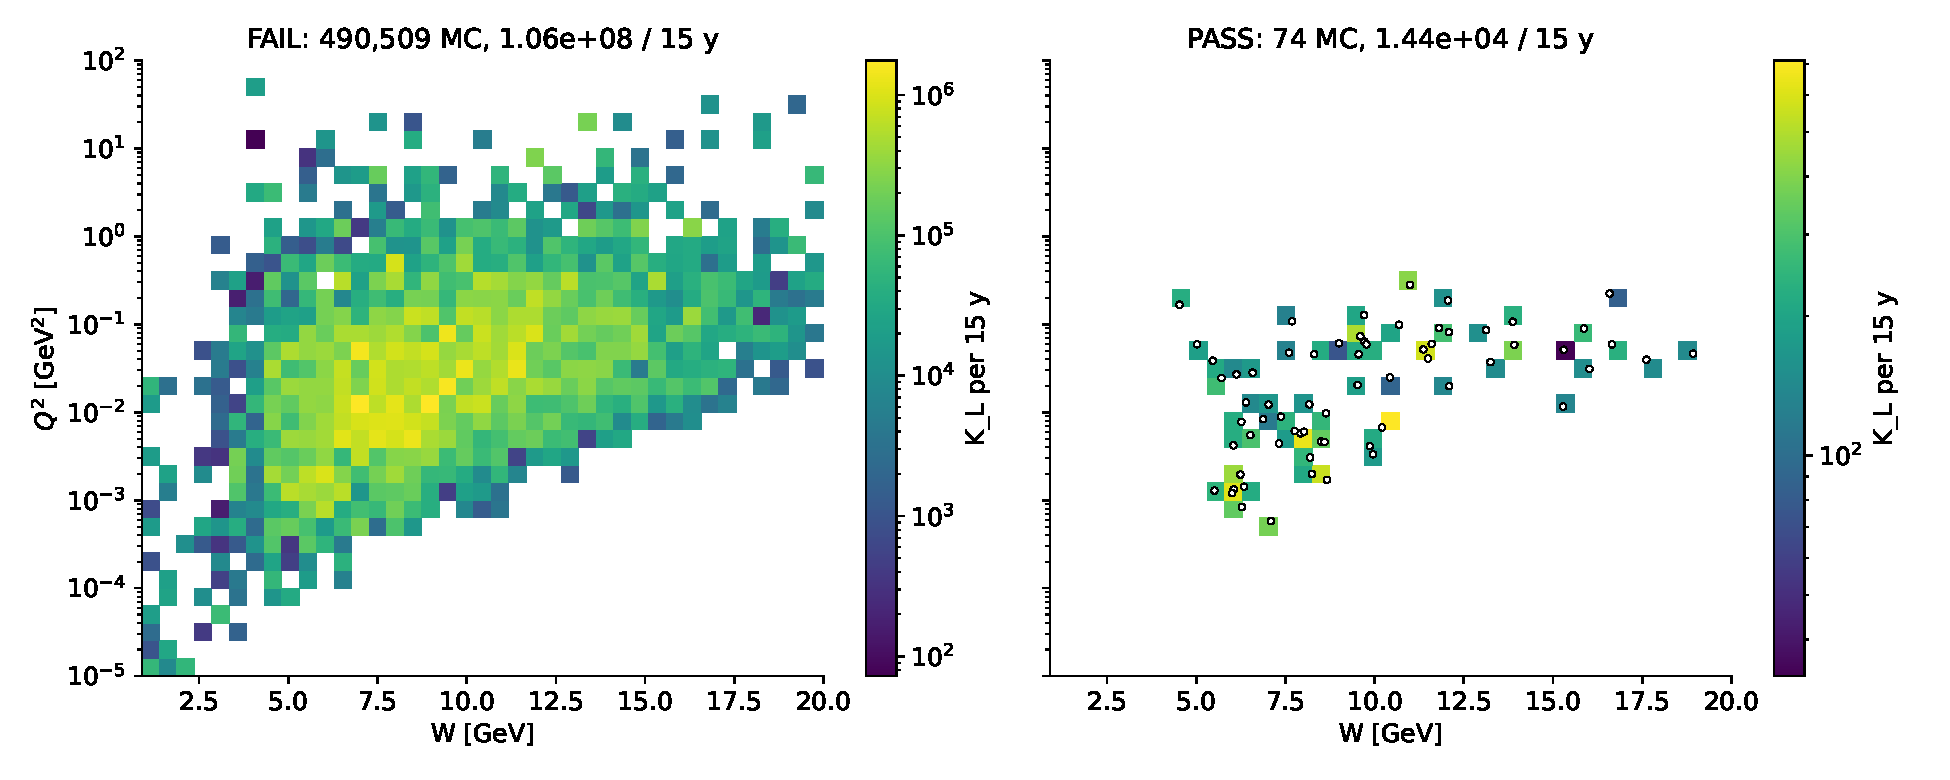
\includegraphics[width=0.80\linewidth,height=100pt,keepaspectratio]{figs/s40d_kl_q2_vs_w.pdf}\par}
\vspace{2pt}
\begin{minipage}[t]{0.52\linewidth}\vspace{0pt}
{\fontsize{5.02pt}{6.52pt}\selectfont\setlength{\tabcolsep}{3.51pt}\renewcommand{\arraystretch}{1.30}
\begin{tabularx}{\linewidth}{>{\raggedright\arraybackslash}Xrrr}
\textcolor{muted}{weighted, per 15 y} & \textcolor{muted}{PASS} & \textcolor{muted}{FAIL} & \textcolor{muted}{all MS7 μ int.} \\\headrule
simulated / per 15 y & 74 / 1.44×10\textsuperscript{4} & 4.9×10\textsuperscript{5} / 1.06×10\textsuperscript{8} & 6×10\textsuperscript{7} / 1.4×10\textsuperscript{13} \\\rowrule
Q\textsuperscript{2} median [GeV\textsuperscript{2}] & 0.012 & 0.028 & 0.0011 \\\rowrule
Q\textsuperscript{2} < 0.01 / < 0.1 / > 1 GeV\textsuperscript{2} & 48 / 90 / 0 \% & 28 / 76 / 3.6 \% & 76 / 96 / 0.3 \% \\\rowrule
W median (10–90 \%) [GeV] & 8.6 (6.0–13.9) & 8.7 (5.7–13.4) & 1.5 (1.2–3.7) \\\rowrule
W < 3.5 / 3.5–5 / > 5 GeV & 0 / 1.6 / 98 \% & 0.6 / 4.3 / 95 \% & 89 / 5.4 / 5.6 \% \\\rowrule
ν / y / E\textsubscript{μ} median & 39 GeV / 0.29 / 122 GeV & 40 GeV / 0.40 / 106 GeV & 0.7 GeV / 0.017 / 70 GeV \\\rowrule
\end{tabularx}\par}
\end{minipage}\hfill
\begin{minipage}[t]{0.45\linewidth}\vspace{0pt}
{\fontsize{5.9pt}{7.9pt}\selectfont
\begin{itemize}
  \item \textcolor{cern}{\textbf{PASS and FAIL come from the same region: W > 5 GeV, quasi-real photon (Q\textsuperscript{2} < 0.1 GeV\textsuperscript{2})}}, ν ≈ 40 GeV: 5 \% of the MS7 interactions
  \item PASS is at \textbf{lower Q\textsuperscript{2} and y} and harder muons: a forward K\textsubscript{L} whose decay pair points back to the target (IP < 10 cm)
  \item No PASS event below W = 3.5 GeV: the data-poor low-W region does not affect the selected background
\end{itemize}}
\end{minipage}
\end{btframe}

% ---------------------------------------------------------------- slide 40e: who sees the parent (19 Nov 2026)
\begin{btframe}{7 · Back-up · MS7 K\textsubscript{L} parent}{Selected MS7 K\textsubscript{L}: which detector sees the parent interaction (R2, own hits only)}
{\centering 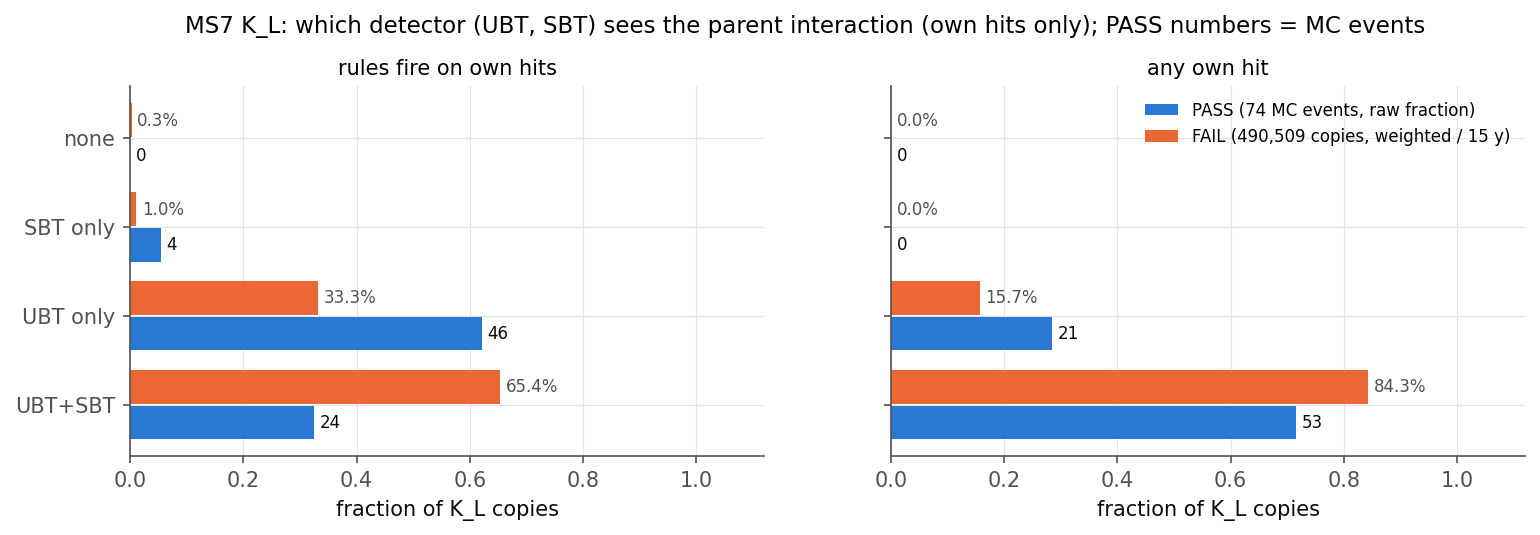
\includegraphics[width=0.84\linewidth]{figs/s40e_categories_nomsms.png}\par}
\vspace{2.46pt}
{\fontsize{6.15pt}{8.60pt}\selectfont
\begin{itemize}
  \item \textbf{UBT V0 rule tags 70 / 74} selected K\textsubscript{L} (FAIL 98.7 \%); the 4 it misses have p\textsubscript{vis} > 20 GeV (p\textsubscript{max} gate) and are tagged by the SBT
  \item SBT rules 28 / 74 (V0 line 18, zone 11, pointing 14); 4 are seen by the SBT only, 46 by the UBT only
  \item Every selected K\textsubscript{L} is tagged by the OR of the R2 rules (74 / 74; FAIL 99.7 \%)
\end{itemize}}
\end{btframe}

% ---------------------------------------------------------------- slide 40f: z dependence in MS7 (19 Nov 2026)
\begin{btframe}{7 · Back-up · MS7 K\textsubscript{L} production z}{Does it depend on where in MS7 the K\textsubscript{L} is made?}
{\centering 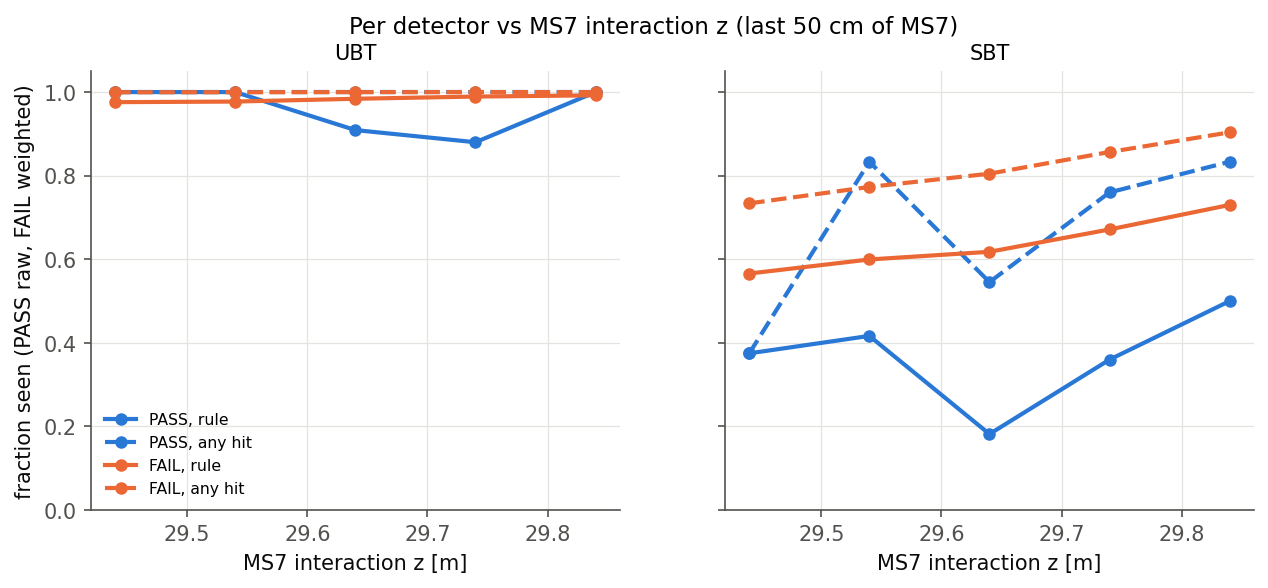
\includegraphics[width=0.90\linewidth,height=125pt,keepaspectratio]{figs/s40f_z_dependence_nomsms.png}\par}
\vspace{2.46pt}
{\fontsize{6.15pt}{8.60pt}\selectfont
\begin{itemize}
  \item \textbf{UBT}: any own hit 100 \% at every z; rule 88–100 \% (the misses are the p\textsubscript{vis} > 20 GeV events)
  \item \textbf{SBT}: more often seen for K\textsubscript{L} made at the end of the iron (FAIL 57 → 73 \%), probably because less iron is left to absorb the products (not yet checked)
  \item 95 \% of the K\textsubscript{L} come from the muon vertex itself (the rest from the shower, within 7 mm of it)
\end{itemize}}
\end{btframe}

% ---------------------------------------------------------------- slide 40d: V0-rule aperture (19 Nov 2026)
\begin{btframe}{7 · Back-up · V0 rule aperture}{V0-rule disc from the kinematic limit: r = 5 cm + p*\textsubscript{max} / p\textsubscript{vis} · Δz, p*\textsubscript{max} = 0.229 GeV}
\begin{minipage}[t]{0.49\linewidth}\vspace{0pt}\centering
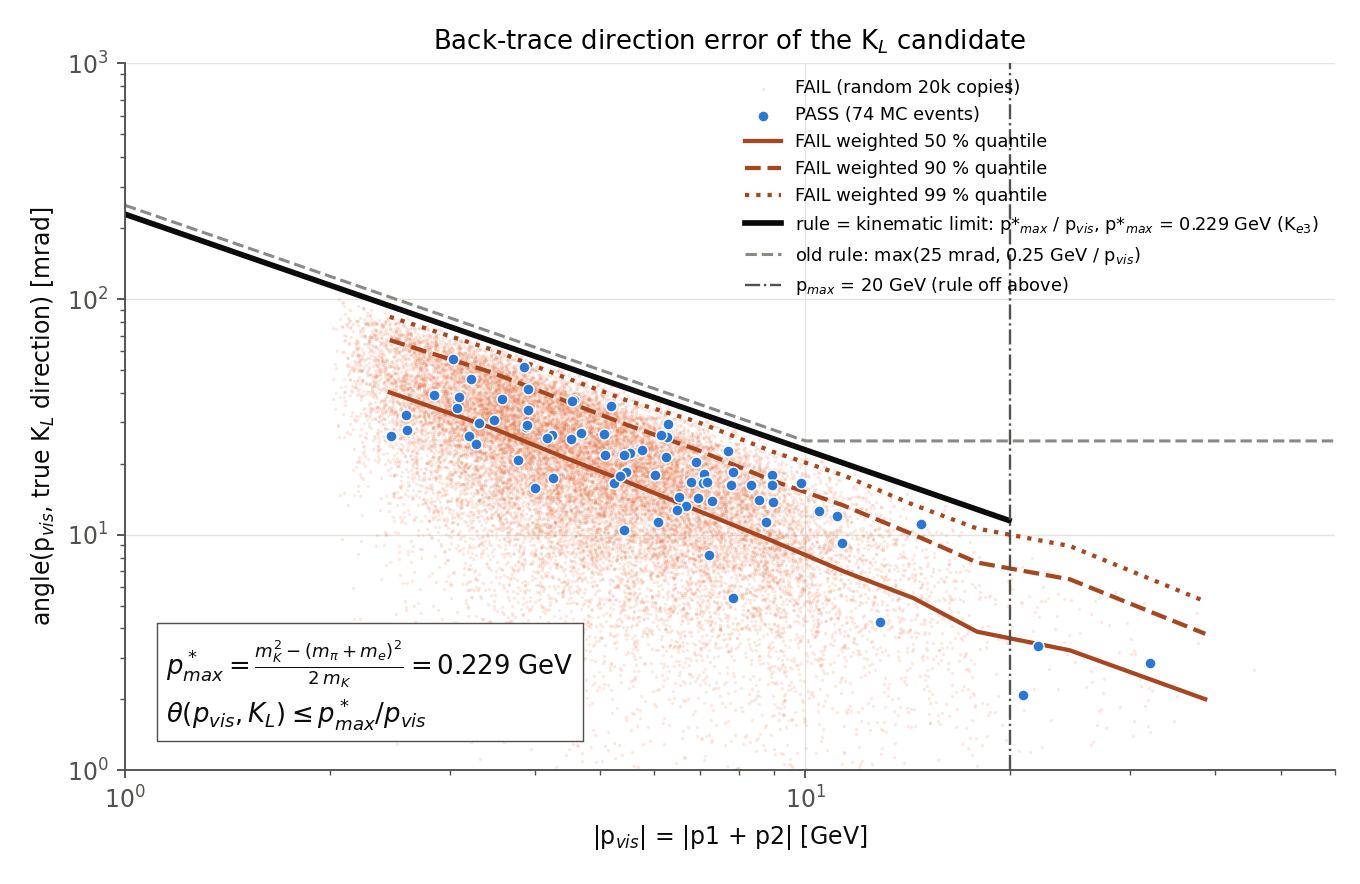
\includegraphics[width=0.88\linewidth]{figs/s40d_angle_vs_pvis_kin.png}
\end{minipage}\hfill
\begin{minipage}[t]{0.49\linewidth}\vspace{0pt}\centering
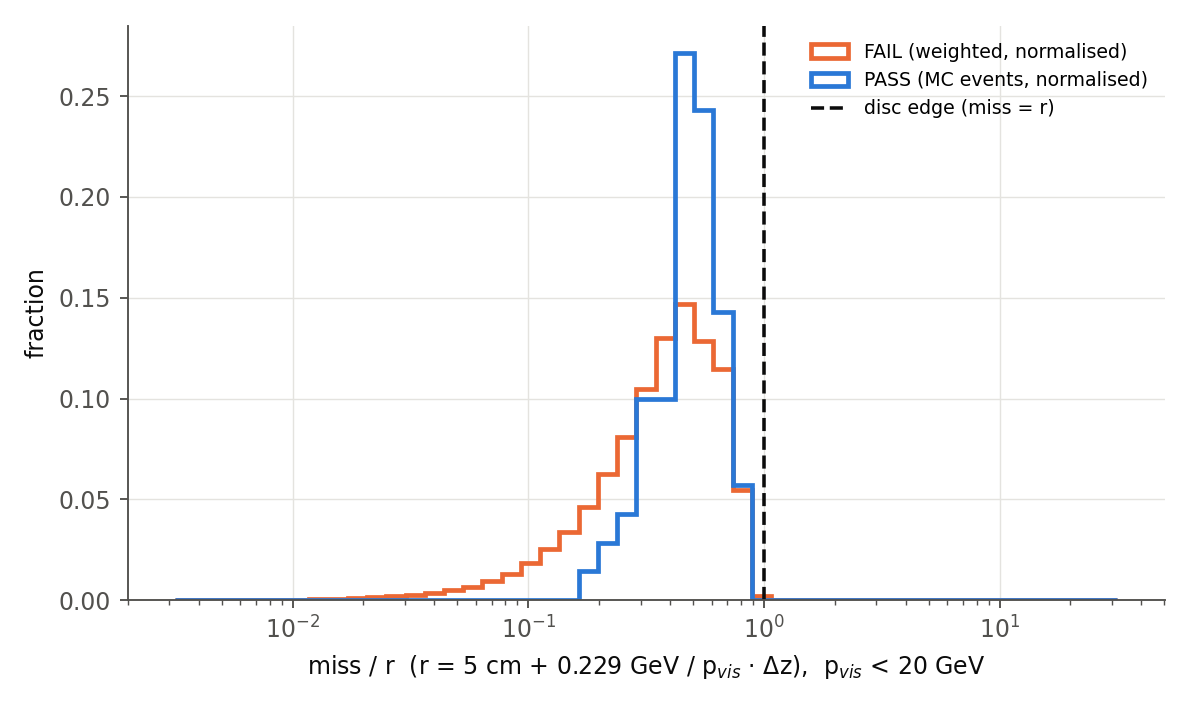
\includegraphics[width=0.88\linewidth]{figs/s40d_miss_over_r_kin.png}
\end{minipage}
\vspace{2.46pt}
{\fontsize{6.15pt}{8.60pt}\selectfont
\begin{itemize}
  \item The pair momentum p\textsubscript{vis} misses the K\textsubscript{L} direction because of the lost ν / π\textsuperscript{0}: selected median 18.5 mrad, 90 \% at 37 mrad; the error falls as 1/p
  \item Kinematic limit: in K\textsubscript{L} → π e ν the lost ν has at most \(p^*_{\max} = (m_K^2 - (m_\pi + m_e)^2)/2m_K\) = \textbf{0.229 GeV} (K\textsubscript{μ3} 0.188, π\textsuperscript{0} lost 0.132), so θ(p\textsubscript{vis}, K\textsubscript{L}) ≤ p*\textsubscript{max} / p\textsubscript{vis}; no tuned parameter, 5 cm = track-search radius
  \item All 4.9×10\textsuperscript{5} K\textsubscript{L} copies inside (max θ · p\textsubscript{vis} = 0.225 GeV). R2 test vs the old max(25 mrad, 0.25/p): MS7 0.81 → 0.84 / 15 y, signal lost 5.21 → 4.97 \% (20 k decays)
\end{itemize}}
\end{btframe}

% ---------------------------------------------------------------- slide 40r: search radius at the tile plane, track rule vs V0 rule (19 Nov 2026)
\begin{btframe}{7 · Back-up · search windows}{Search radius at the UBT tile plane: track rule and V0 rule}
{\centering 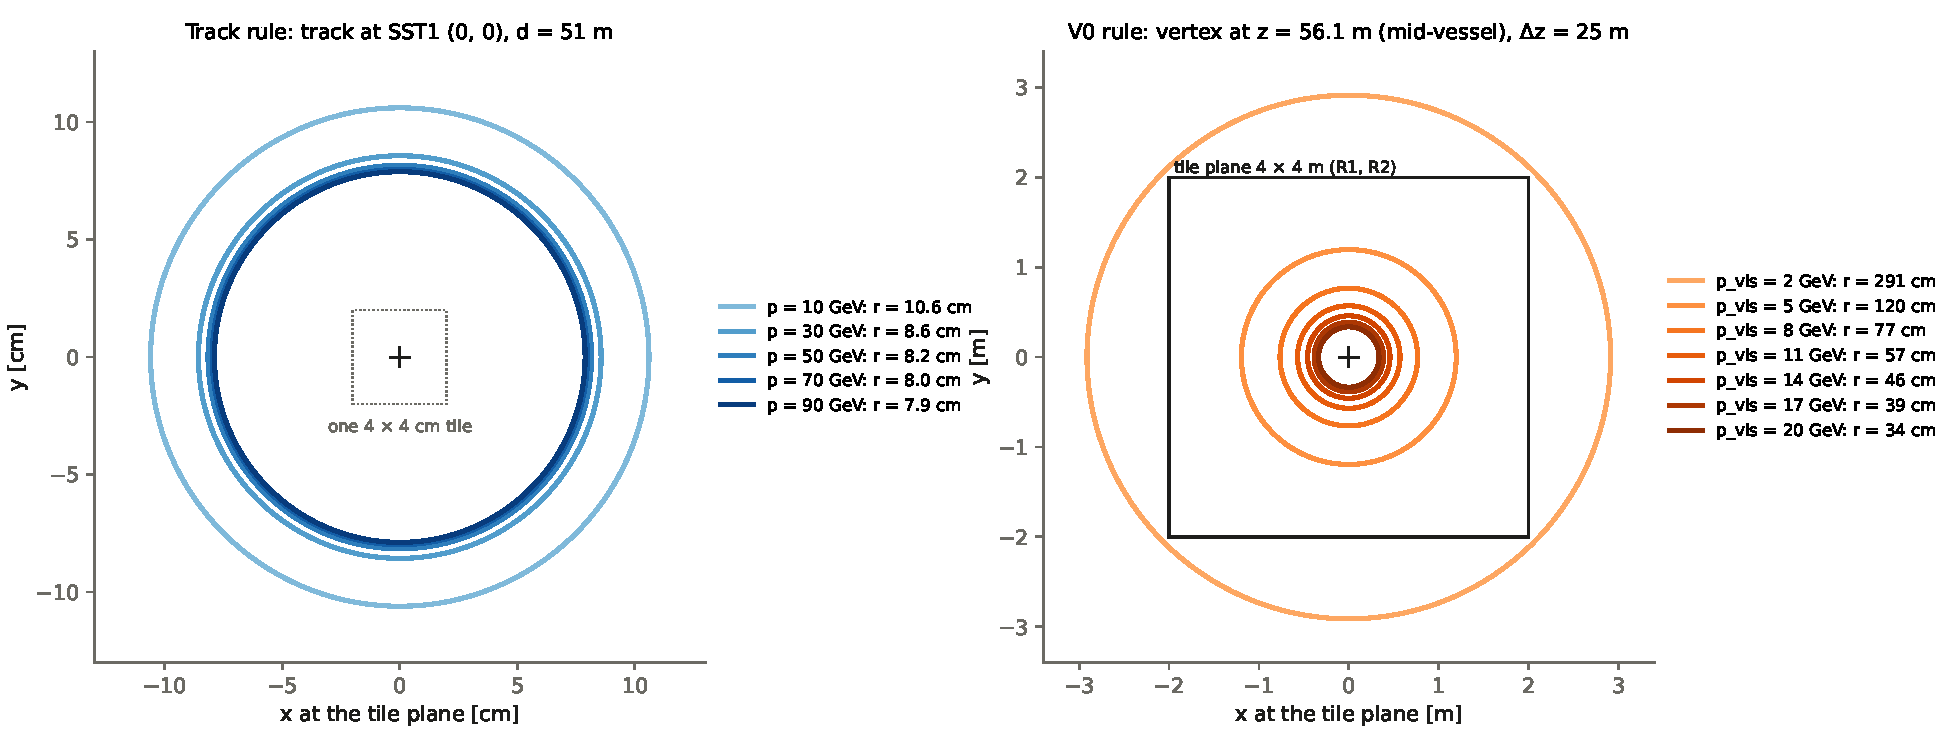
\includegraphics[width=\linewidth,height=136pt,keepaspectratio]{figs/aperture_radii_kin.pdf}\par}
\vspace{2.46pt}
{\fontsize{5.9pt}{7.9pt}\selectfont
\begin{itemize}
  \item \textbf{Track rule} (left), traced back from SST1 (82.08 m) over d = 51 m: r = 5 cm + (0.5 + 6 GeV / p) mrad × d → \textbf{10.6 cm at 10 GeV}, 7.9 cm at 90 GeV (straws, 30.73 m: +0.2 mm)
  \item \textbf{V0 rule} (right), vertex on axis in the middle of the vessel (z = 56.13 m, Δz = 25 m): r = 5 cm + 0.229 GeV / p\textsubscript{vis} × Δz → \textbf{2.9 m at 2 GeV}, 1.2 m at 5 GeV, 77 cm at 8 GeV, 46 cm at 14 GeV, \textbf{34 cm at 20 GeV}; the rule is off above p\textsubscript{vis} = 20 GeV
  \item The V0 disc is 3–30 × wider than a track window: it collects the most random hits, hence most of the signal loss (2 GeV: the disc covers the whole 4 × 4 m plane)
\end{itemize}}
\end{btframe}

% ---------------------------------------------------------------- slide 25: Slow MS7 KL escaped the 25 mrad cone: three fixes, A + C adopted
\begin{btframe}{7 · Back-up · V0 rule history}{Slow MS7 K\textsubscript{L} escaped the 25 mrad cone: three fixes, A + C adopted}
\noindent \begin{minipage}[t]{\dimexpr(0.2500\linewidth-0.2500\dimexpr14.22pt\relax)}\vspace{0pt}\raggedright
{\centering \fontsize{4.55pt}{6.15pt}\selectfont \textcolor{purple}{\textbf{25 mrad cone: misses (slow K\textsubscript{L})}}\par}
\vspace{0.27pt}
{\centering 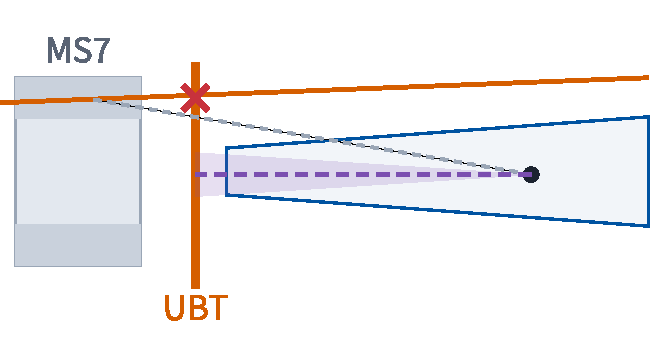
\includegraphics[width=1.00\linewidth,height=63.73pt,keepaspectratio]{figs/s24_sk1.pdf}\par}
\end{minipage}%
\hfill%
\begin{minipage}[t]{\dimexpr(0.2500\linewidth-0.2500\dimexpr14.22pt\relax)}\vspace{0pt}\raggedright
{\centering \fontsize{4.55pt}{6.15pt}\selectfont \textcolor{purple}{\textbf{A: cone max(25 mrad, 0.25 GeV / p\textsubscript{vis})}}\par}
\vspace{0.27pt}
{\centering 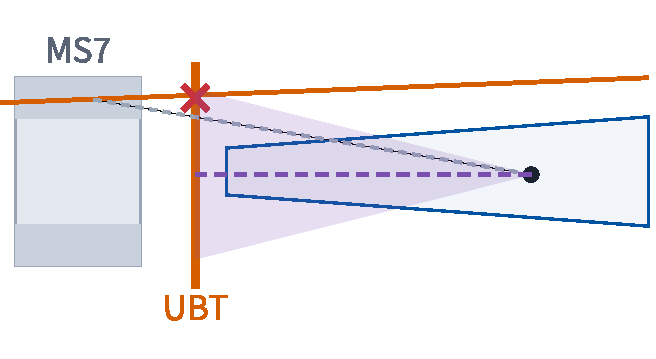
\includegraphics[width=1.00\linewidth,height=63.73pt,keepaspectratio]{figs/s24_sk2.pdf}\par}
\end{minipage}%
\hfill%
\begin{minipage}[t]{\dimexpr(0.2500\linewidth-0.2500\dimexpr14.22pt\relax)}\vspace{0pt}\raggedright
{\centering \fontsize{4.55pt}{6.15pt}\selectfont \textcolor{purple}{\textbf{B: extra lines to the yoke legs}}\par}
\vspace{0.27pt}
{\centering 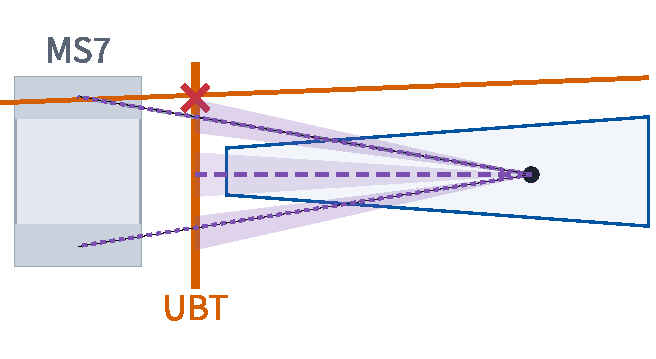
\includegraphics[width=1.00\linewidth,height=63.73pt,keepaspectratio]{figs/s24_sk3.pdf}\par}
\end{minipage}%
\hfill%
\begin{minipage}[t]{\dimexpr(0.2500\linewidth-0.2500\dimexpr14.22pt\relax)}\vspace{0pt}\raggedright
{\centering \fontsize{4.55pt}{6.15pt}\selectfont \textcolor{purple}{\textbf{C: window opened by the K\textsubscript{L} flight time}}\par}
\vspace{0.27pt}
{\centering 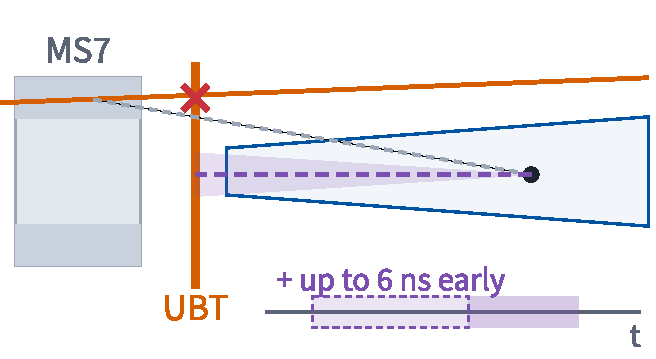
\includegraphics[width=1.00\linewidth,height=63.73pt,keepaspectratio]{figs/s24_sk4.pdf}\par}
\end{minipage}\par
\vspace{2.46pt}
{\fontsize{4.37pt}{5.68pt}\selectfont\setlength{\tabcolsep}{3.06pt}\renewcommand{\arraystretch}{1.42}
\begin{tabularx}{\linewidth}{>{\raggedright\arraybackslash}Xrrrr}
\textcolor{muted}{variant} & \textcolor{muted}{signal lost F / P} & \textcolor{muted}{MS7 μ tagged} & \textcolor{muted}{own hits only} & \textcolor{muted}{MS7 μ left / 15 y} \\\headrule
25 mrad (before the fix) & 5.3 / 9.4 \% & 66 \% & 63 \% & 8.1×10\textsuperscript{3} \\\rowrule
A: 1/p cone & 5.4 / 10.5 \% & 100 \% & 100 \% & 0.63 \\\rowrule
B: yoke lines & 12.1 / 25.1 \% & 100 \% & 100 \% & 0.48 \\\rowrule
C: time of flight & 4.9 / 7.6 \% & 68 \% & 67 \% & 7.8×10\textsuperscript{3} \\\rowrule
\rowcolor{tint}\bfseries A + C (adopted) & \bfseries 5.0 / 8.4 \% & \bfseries 100 \% & \bfseries 100 \% & \bfseries 0.67 \\\rowrule
B + C & 11.5 / 21.8 \% & 100 \% & 100 \% & 0.48 \\\rowrule
\end{tabularx}\par}
\end{btframe}

% 

% ---------------------------------------------------------------- slide 42: the OR of the rules (19 Nov 2026)
\begin{btframe}{7 · Back-up · OR of the rules}{All rules run on every candidate, in parallel: tagged = OR}
{\centering
\begin{tikzpicture}[x=1pt,y=1pt,font=\fontsize{5.2pt}{6.4pt}\selectfont,
  box/.style={line width=0.5pt,rounded corners=1.5pt,fill=white,align=center,inner sep=2.2pt,text width=140pt},
  arr/.style={-{Stealth[length=2.6pt]},line width=0.5pt,color=ink}]
  \node[draw=cern,fill=tint,line width=0.5pt,rounded corners=1.5pt,align=center,inner sep=2.5pt,text width=62pt] (c) at (0,0)
    {\textbf{\textcolor{cern}{candidate}}\\2 tracks at SST1\\vertex in the vessel};
  \node[box,draw=cern] (t) at (135,32) {\textbf{\textcolor{cern}{Track rule}} -- each track separately\\line from SST1 back\\r = 5 cm + (0.5 + 6 GeV/p) mrad · d};
  \node[box,draw=purple] (v) at (135,0) {\textbf{\textcolor{purple}{V0 rule}} -- the pair as one neutral (p\textsubscript{vis} < 20 GeV)\\line from the vertex along p\textsubscript{vis}, early time window};
  \node[box,draw=green] (s) at (135,-32) {\textbf{\textcolor{green}{SBT rules}} -- pointing, V0 line, zone};
  \node[circle,draw=ink,line width=0.6pt,fill=white,inner sep=1.2pt,font=\fontsize{6pt}{7pt}\selectfont\bfseries] (or) at (250,0) {OR};
  \node[draw=red,fill=red!8,line width=0.5pt,rounded corners=1.5pt,align=center,inner sep=2.5pt,text width=52pt] (out) at (310,0)
    {\textbf{\textcolor{red}{tagged}}\\any rule found a hit};
  \foreach \b in {t,v,s}{\draw[arr] (c.east) -- (\b.west); \draw[arr] (\b.east) -- (or);}
  \draw[arr] (or) -- (out.west);
\end{tikzpicture}\par}
\vspace{4pt}
{\fontsize{5.31pt}{6.90pt}\selectfont\setlength{\tabcolsep}{3.72pt}\renewcommand{\arraystretch}{1.42}
\begin{tabularx}{\linewidth}{>{\raggedright\arraybackslash}X>{\raggedright\arraybackslash}X>{\raggedright\arraybackslash}X}
\textcolor{muted}{what made the candidate} & \textcolor{muted}{what is upstream} & \textcolor{muted}{rule that finds it} \\\headrule
muon pairs from outside, rock tracks, bounced muons & each track came from upstream & track rule \\\rowrule
muon interaction in the helium / walls & the incoming muon, nearly along the outgoing one & track rule (a kinked one escapes) \\\rowrule
K\textsubscript{L} / neutrals from MS7 or the SBT material & nothing on the tracks' lines; the parent's products along p\textsubscript{vis} & V0 rule, SBT V0 line \\\rowrule
\rowcolor{tint}signal (HNL, …) & nothing & none -- a random hit in any window = signal lost \\\rowrule
\end{tabularx}\par}
\vspace{3pt}
{\fontsize{6.15pt}{8.60pt}\selectfont
\begin{itemize}
  \item No “first the tracks, then the V0 rule”: every window is open at the same time; a rule built for another source simply finds nothing
  \item Tables quote the extra candidates each rule adds (e.g. V0 rule: MS7 1.5×10\textsuperscript{4} → 0.82); the signal loss includes all windows together, which is why p\textsubscript{max} keeps fast (signal-like) pairs out of the V0 disc
\end{itemize}}
\end{btframe}

\end{document}
